\documentclass[french]{article}
\usepackage[T1]{fontenc}
\usepackage[utf8]{inputenc}
\usepackage{lipsum}
\usepackage{lmodern}
\usepackage{geometry}
\usepackage{babel}
\usepackage{graphicx}
\usepackage{lastpage}
\usepackage{ragged2e}
\usepackage{enumitem}
\usepackage[normalem]{ulem}
\usepackage{hyperref} % pour \url{URL}
\usepackage{color} % pour \textcolor{color}{text}
\usepackage{listings} % pour afficher du code
\usepackage{longtable} % pour l'environnement longtable
\usepackage{float} % pour des figures non flottantes
\usepackage{amsmath}
\usepackage{verbatim} % pour les graphes
\usepackage{caption} % figure et subfigure pour mettre les images côtes à côtes
\usepackage{subcaption}
\usepackage{dirtree}
\usepackage{pdfpages}

% Grammaire EBNF
\usepackage{syntax}
\setlength{\grammarparsep}{5pt plus 1pt minus 1pt}
\setlength{\grammarindent}{11em}

% Dessin avec tikz
\usepackage{tikz}
\usepackage{forest}
\usetikzlibrary{shapes,arrows,positioning,shadows,matrix,automata}

% Matrices
\usepackage{kbordermatrix}% http://www.hss.caltech.edu/~kcb/TeX/kbordermatrix.sty

% Largeur de colonnes de tableau fixes
\usepackage{array}
\newcolumntype{L}[1]{>{\raggedright\let\newline\\\arraybackslash\hspace{0pt}}m{#1}}
\newcolumntype{C}[1]{>{\centering\let\newline\\\arraybackslash\hspace{0pt}}m{#1}}
\newcolumntype{R}[1]{>{\raggedleft\let\newline\\\arraybackslash\hspace{0pt}}m{#1}}

% Style C++
\lstset{
	language=C++,
	tabsize=2,
	basicstyle=\small\ttfamily,
	keywordstyle=\color{blue},
	stringstyle=\color{red},
	commentstyle=\color{black!40},
	morecomment=[l][\color{black!50}]{\#},
	gobble=10,
	frame=single,
	otherkeywords={constexpr,std,string,vector,map,pair,size\_t,function,remove\_const,remove\_reference}
}

\geometry{
	a4paper,
	total={210mm,297mm},
	left=20mm,
	right=20mm,
	top=20mm,
	bottom=20mm,
}

\usepackage{fancyhdr}
\pagestyle{fancy}
\setlist[enumerate,1]{leftmargin=2cm}

% Entêtes
\lhead{Browne, Champion, Djomo,\\Hardy, Richoz, Rochat}
\chead{}
\rhead{PRO: Rapport}
\renewcommand{\headrulewidth}{0.4pt}
\renewcommand{\footrulewidth}{0.4pt}

\begin{document}
	
	
	% Titre du document
	\title{GraphY} % ou un autre nom
	\author{Rapport\\ 
		Projet de semestre\\
		Browne Champion Djomo Hardy Richoz Rochat\\
		Resp. René Rentsch\\
		HEIG-VD}
	\date{\today} % date du jour
	\maketitle
	\thispagestyle{empty}
	
	\newpage
	\thispagestyle{empty}
	$ $
	\newpage
	
	% Pour tout le document
	\justify
	\normalsize
	
	% Tables des matières
	\tableofcontents
	
	\newpage
	
	\section*{Remerciements}
	Nous tenons tout d'abord à remercier M. Prof. René Rentsch pour son suivi et ses conseils durant toute la période du travail. Nous voulons aussi remercier M. Prof. Claude Evéquoz pour son aide à la vérification de la grammaire de notre langage. Enfin, merci également à M. Prof. Jean-François Hêche pour ses conseils sur l'implémentation des algorithmes de graphes.
	
	\section{Introduction}
	Dans le cadre du cours PRO en deuxième année du cursus de Bachelor de la HEIG-VD, il a été demandé de réaliser un projet de semestre sur une période de 10 semaines. Après l'acceptation du cahier des charges à la semaine 4, le projet a pu débuter. Celui-ci porte sur une application permettant de traiter des graphes, de lancer des algorithmes dessus, de les dessiner et enfin de pouvoir les exporter en format d'image vectoriel.
	
		\subsection{Objectif}
		Les objectifs principaux du rapport peuvent être décomposés en quatre parties. Premièrement, il doit être possible de saisir un graphe et qu'il soit stocké dans l'application. Ensuite, des algorithmes classiques des graphes (Dijkstra, parcours en profondeur/largeur, etc...) doivent pouvoir être appliqués au graphe précédemment saisi. Puis, il doit pouvoir être dessiné et remanié avec le curseur pour permettre de l'exporter en image vectorielle. Enfin, toutes ces parties doivent être coordonnées au moyen d'un langage spécifique à l'application.\\
		Toutes les spécifications précises sont disponibles dans le cahier des charges fourni en annexe.
		
		\subsection{Conception générale}
		La conception générale de l'application a été faite en couches pour deux raisons. Premièrement, cette décomposition permet de répartir le travail plus facilement et de manière plus efficace entre les personnes. En effet, cela réduit les dépendances au niveau du développement et donc le temps passé à attendre sur le travail d'un autre, ainsi que le nombre de conflits sur le gestionnaire de versions. Deuxièmement, cette approche permet d'avoir des composants indépendants (voir \textbf{figure \ref{couchesLogicielles}}) et donc réutilisables, puisque les couches inférieures n'ont pas connaissance des couches supérieures et proposent des interfaces indépendantes.\\
		La première couche à mentionner, celle avec laquelle l'utilisateur interagit est l'interface graphique (GUI). Celle-ci propose une console pour saisir des commandes, ainsi que quelques menus. Elle est également liée à l'aide utilisateur, qui comporte une fenêtre de navigation HTML. La GUI est interfacée avec l'interpréteur qui vérifie la validité des commandes tapées et renvoie un message d'erreur en cas de mauvaise saisie. Si, au contraire, la commande est correcte, l'interpréteur la transmet soit à la couche graphe, soit à la couche algorithme. En parallèle à cet interpréteur, la couche de dessin accède également à la couche graphe pour en dessiner des représentations.
		
		\begin{figure}[H]
			\centering
			\begin{tikzpicture}
			\draw (0,0) rectangle (4,1) node[pos=.5] {Algorithms};
			\draw (0,-2) rectangle (12,-1) node[pos=.5] {Graphs};
			\draw (0,2) rectangle (7,3) node[pos=.5] {\textit{EGLI}};
			\draw (0,4) rectangle (7,7) node[pos=.5] {\textit{GUI}};
			\draw (8,4) rectangle (12,5) node[pos=.5] {Visualization};
			\draw (8,6) rectangle (12,7) node[pos=.5] {User help};
			
			\draw[->] (3.5,4) -- (3.5,3);
			\draw[->] (2,2) -- (2,1);
			\draw[->] (2,0) -- (2,-1);
			\draw[->] (5.5,2) -- (5.5,-1);
			\draw[->] (10,4) -- (10,-1);
			\draw[->] (7,4.5) -- (8,4.5);
			\draw[->] (7,6.5) -- (8,6.5);
			\end{tikzpicture}
			\caption{Couches logicielles}
			\label{couchesLogicielles}
		\end{figure}
		
		Ce rapport est organisé de manière à partir des couches hautes (\textit{GUI}) pour descendre petit à petit dans les couches basses.
	
	\section{Cadre de développement} 
		L'application est développée à l'aide du langage C++ (standard C++11) et de la bibliothèque Qt (version 5.5.1). Elle est compilée avec MinGW 4.9.2 32 bits sur Windows. La version de la librairie Boost utilisée pour le parseur est la 1.60.0. Afin que le code source soit écrit dans le même style par tous les membres du groupe, nous avons décidé d'utiliser le Coding Style de Qt \cite{qtStyle} qui correspond bien à nos besoins. Nous avons également utilisé GitHub pour gérer la mise en commun du code.
			
	\section{Interface}
	\subsection{Fenêtre principale}
	\subsubsection{Conception générale}
	Afin de mettre en place un principe de session de travail, un système d'onglets multiples est proposé, chacun contenant une console, afin de pouvoir travailler en parallèle sur plusieurs graphes.
	\subsubsection{Console}
	Qt ne proposant pas directement de Widget faisant office de console, il a fallu en créer un adapté au besoin de l'application. La base de la console est un QTextEdit, un composant permettant la saisie libre de texte. Le QTextEdit autorisant justement de saisir du texte où bon nous semble, il a fallu mettre en place des fonctionnalités limitant l'utilisateur dans les endroits où il peut saisir du texte. Dans un premier temps, un buffer contenant le texte saisi par l'utilisateur a été implémenté.\\
	Ensuite, pour synchroniser les données réellement saisies et l'affichage, un curseur géré manuellement a été mis en place. En effet le curseur de base est sensible au clic de la souris, ce qui lui permettrait de pouvoir insérer du texte n'importe où. Grâce au curseur créé, on s'assure que le texte sera inséré au bon endroit dans l'affichage.\\
	Le menu contextuel par défaut aussi posait problème, car il implémentait des fonctionnalités allant à l'encontre de l'intégrité de la console, comme par exemple la fonction "couper" ou encore "supprimer" qui permettait d'enlever du texte de la console. Un nouveau menu, proposant uniquement des fonctionnalités ne supprimant pas l'affichage actuel, a été créé. Ainsi, grâce à celui-ci, il est possible de "Copier", "Coller", et "Sélectionner tout" du texte d'une console. La fonction "Coller" insère le texte à partir du curseur géré manuellement pour empêcher des incohérences dans l'application.
	\subsection{Auto complétion}
	\subsubsection{Implémentation du dictionnaire}
	La première étape pour permettre l'implémentation de l'auto complétion est le choix d'une structure de données adéquate. Après quelques recherches, le \textit{ternary search tries} se montre le plus adéquat. En effet, sa mise en œuvre permet une recherche très rapide. Pour une recherche réussie (\textit{search hit}), sa complexité est de l'ordre de $O(L + ln(N))$ avec $L$ la longueur de la chaine recherchée et $N$ le nombre de mots dans le dictionnaire \cite{tries}. Une recherche ratée (\textit{search miss}) prend quant à elle $O(ln(N))$. Il est vrai qu'une hash map effectue toutes ses opérations en moyenne en $O(L)$, mais le temps de hachage et non-négligeable et la performance globale en temps et en espace mémoire est souvent moins bonne \cite{sedgewick}.
	
	\subsubsection{Auto-complétion dans la GUI}
	Au final, l'auto-complétion proposée par Qt a pu être adaptée à l'utilisation dans la console principale, ce qui a rendu les efforts consacrés à l'implémentation d'un dictionnaire efficace inutiles. Le comportement de l'auto-complétion n'est pas exactement celui initialement prévu, mais son utilisation a permis un gain de temps global.
	
	\subsection{Aide utilisateur}
	\subsubsection{Conception générale}
	Les fichiers d'aide utilisateur ont été écrits au format HTML, afin qu'ils soient rapidement rédigés et que l'utilisateur puisse naviguer d'une page à l'autre. L'interface de l'aide contient également une barre de recherche qui utilise un fichier de mots-clés pour effectuer ces recherches. Ceci a été fait, plutôt que de chercher le texte dans les fichiers, afin qu'une recherche avec un mot commun du langage, tel que \textit{graph}, \textit{edge} ou \textit{vertex} n'affiche pas toutes les pages de l'aide, puisque ces mots se trouvent dans la majorité des fichiers.

	\section{Représentation graphique des graphes}
	\subsection{Widget de visualisation}
	\subsubsection{Fonctionnement de Qt}
	Qt possède un système de dessin complexe, le \textit{Graphics View Framework}. Cet outil est basé sur le principe suivant : trois types d'éléments se partagent différentes responsabilités. \\
	
	\textbf{La scène (classe QGraphicsScene)} :
	\begin{itemize}
		\item Fournit une interface afin de gérer les éléments graphiques.
		\item Gère les états des éléments graphiques.
		\item Propage les événements aux éléments graphiques.
	\end{itemize}
	
	La scène est donc un conteneur pour tout ce qui sera visible par l'utilisateur. Qt fournit des méthodes pour ajouter, supprimer des éléments, mais aussi pour trouver un élément à une certaine coordonnée. Lors de la sélection d'un élément, c'est également la scène qui s'occupe de l'informer d'une action. \\
	
	\textbf{La vue (classe QGraphicsView)} : \\
	La vue se charge d'afficher le contenu d'une scène (plusieurs vues peuvent très bien afficher la même scène). Ici, la scène peut être perçue comme un modèle du design MVC. \\
	Elle s'occupe d'afficher tout ou une partie de la scène, c'est à dire que si cette dernière est grande, trop grande pour la fenêtre ou pour la zone à disposition, la vue va s'occuper d'ajouter des barres de défilement. Ceci engendre que les coordonnées peuvent différer entre une vue et sa scène. La vue recevant en premier les actions de l'utilisateur, va les transmettre à la scène en prenant soin d'adapter les coordonnées si besoin. Par exemple, un clic en haut à gauche de la fenêtre sera en coordonnées (0,0) pour la vue, mais si l'utilisateur a auparavant scrollé horizontalement et/ou verticalement, la coordonnée réelle du clic sur la scène pourrait être (0,100), (130, 10), etc. Cette adaptation est donc extrêmement importante. Des méthodes sont également mises à disposition par Qt afin de manuellement demander la correspondance d'une coordonnée vue -> scène ou scène -> vue. \\
	
	\textbf{Les éléments graphiques (classe QGraphicsItem et sous-classes)} : \\
	Ces classes représentent des éléments graphiques de base, une ellipse (QGaphicsEllipseItem), un rectangle (QGraphicsRectItem), un texte (QGraphicsTextItem), etc. Il est possible de les paramétrer en leur fournissant un objet QPen personnalisé (pour le contour) et/ou un objet QBrush (pour le fond) et en utilisant leur interface publique respective. Il est également possible de spécialiser une classe de Qt afin de créer ses propres éléments.
	Ces objets possèdent une fois de plus leur propre système de coordonnées. La position qu'il leur est attribuée par la scène devient leur point d'origine et là aussi des méthodes permettent des conversions.
	
	\pagebreak
	
	\subsubsection{Diagramme de classe}
	\begin{figure}[H]
		\centering
		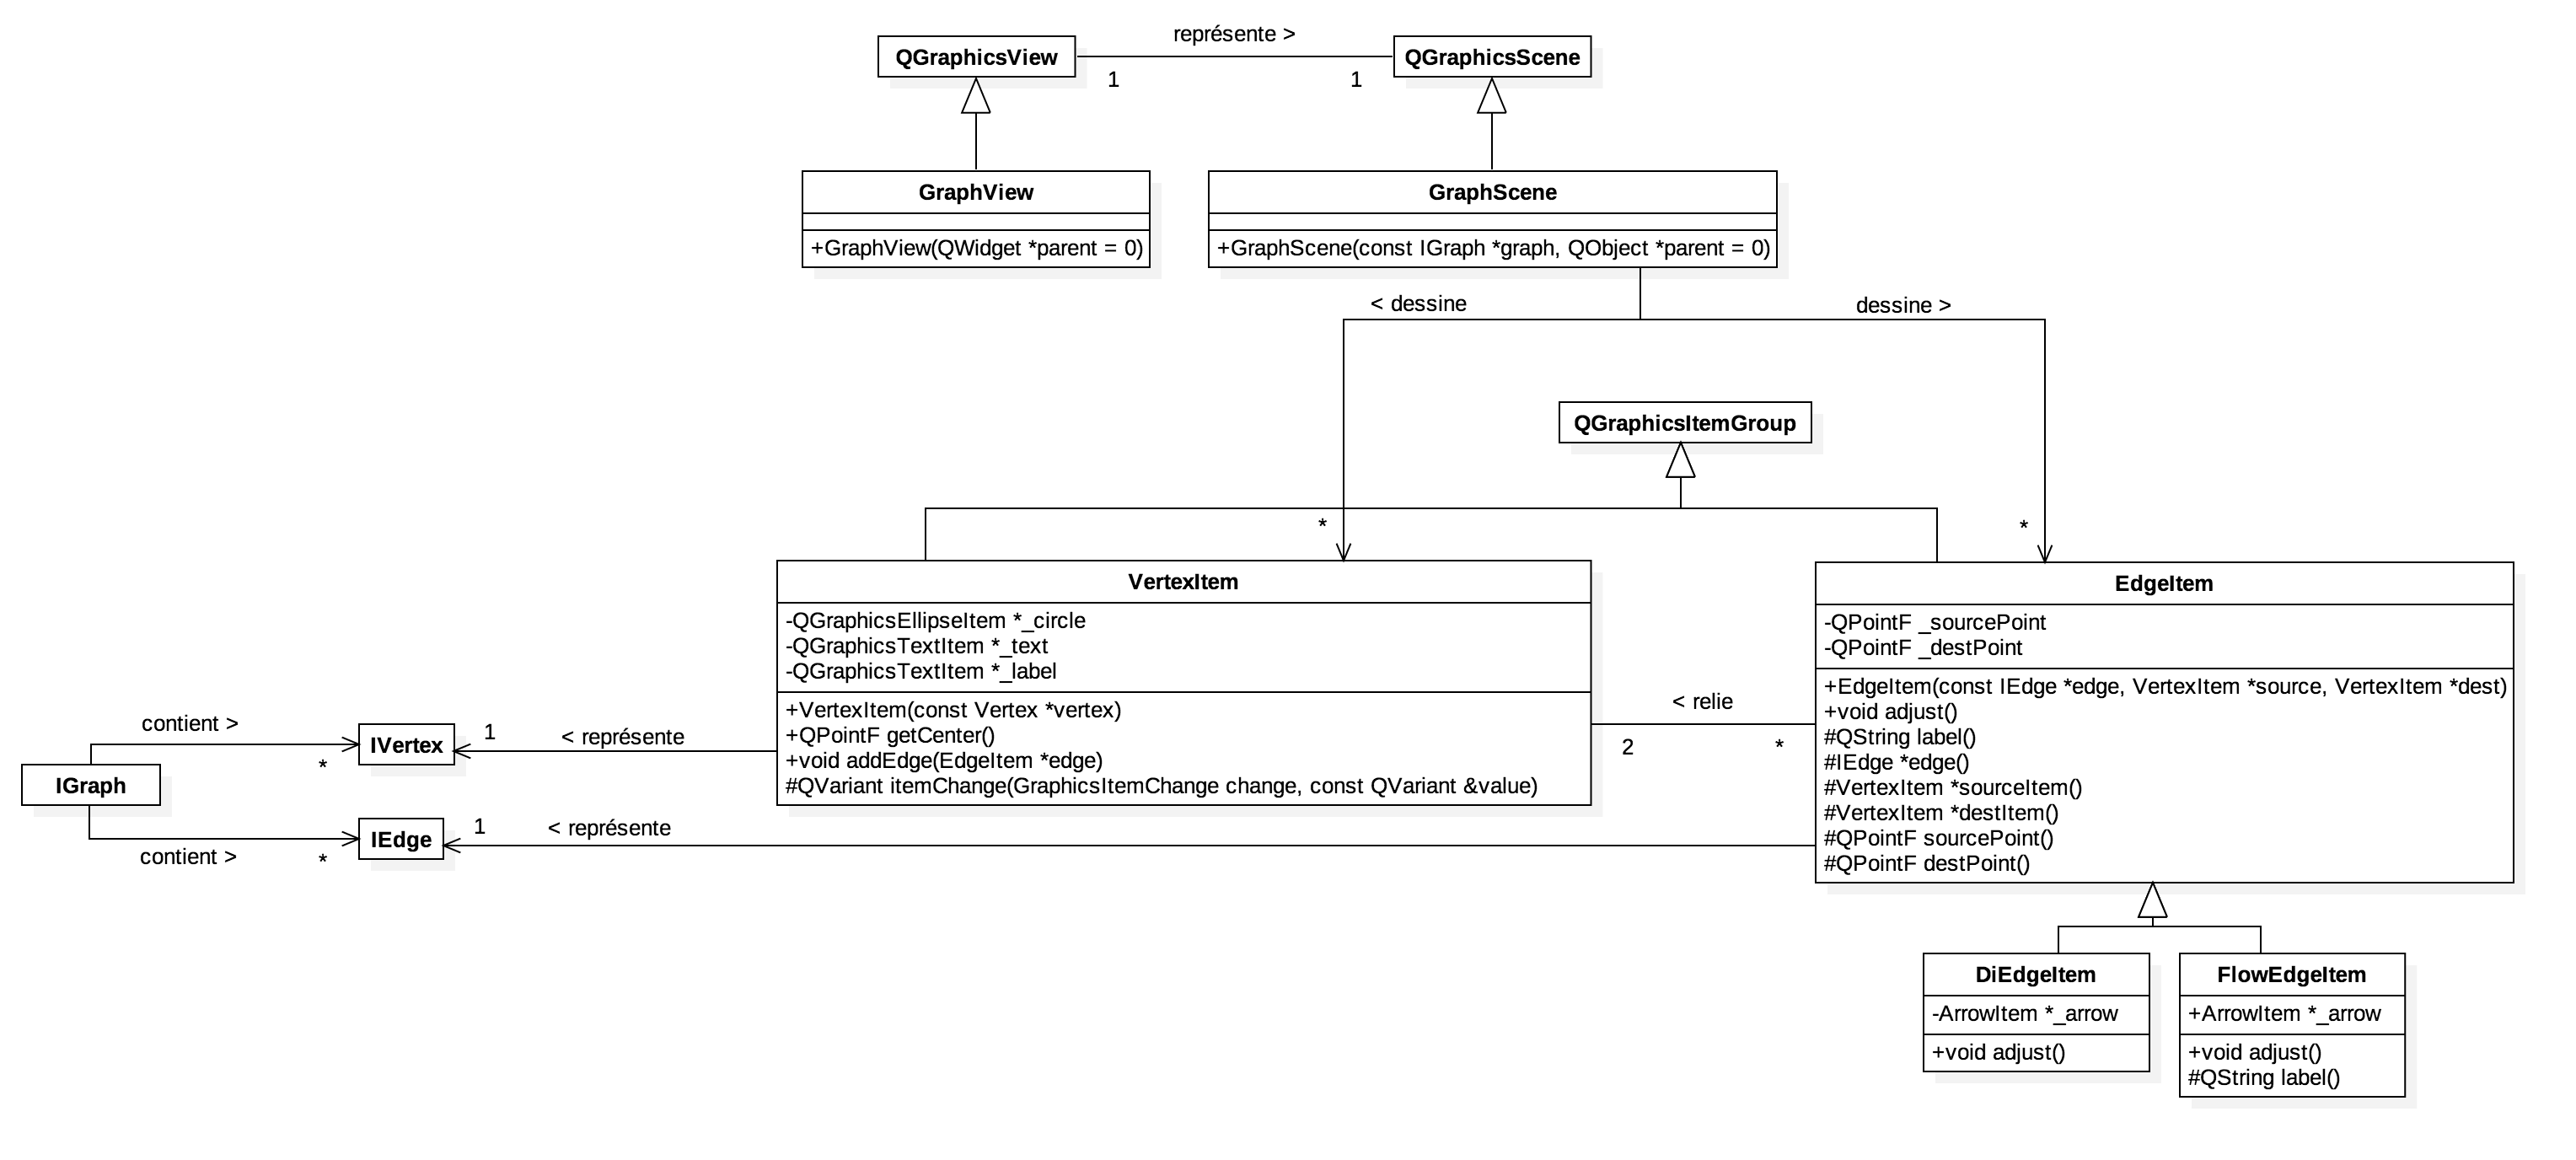
\includegraphics[width=0.9\textheight,angle=90]{Conception/visualization/visualization.png}
		\caption{Diagramme de classes de la représentation des graphes}
	\end{figure}
	
	\pagebreak
	
	Afin de respecter la philosophie de Qt, j'ai créé des classes spécialisées pour chaque partie. La classe \textbf{GraphView} n'a pas forcément d'utilité pour l'instant, mais pour l'éventuel avenir du projet, celle-ci permettra de gérer des événements plus précis (actuellement nous n'avons implémenté que le drag and drop des sommets et ceci est automatiquement géré par Qt). \\
	La classe \textbf{GraphScene} prend en paramètre un pointeur de IGraph. C'est cette objet qui va s'occuper de créer tous les éléments graphiques nécessaires à sa représentation. \\
	Puis les éléments graphiques \textbf{VertexItem} et \textbf{EdgeItem} (ainsi que ses sous-classes \textbf{DiEdgeItem} et \textbf{FlowEdgeItem}) permettent respectivement de dessiner les sommets et les arcs/arêtes. Ces classes ne sont pas directement de type QGraphcsItem, mais de QGraphicsItemGroup qui est en fait un conteneur de plusieurs QGraphcsItem. En effet, un sommet est composé d'un cercle (réellement d'une ellipse) d'un texte pour l'identifiant affiché et d'un autre texte pour son label. Les arêtes (EdgeItem) qui sont des simple lignes avec un label, les arcs (DiEdge) qui ajoutent une flèche pour la direction et les flux (FlowEdge) qui ajout également une flèche, mais aussi les capacités. Chacun des éléments graphiques ajoute et gère tous les autres éléments graphiques dont il a besoin. \\
	
	Finalement, la scène se charge de donner une position aux sommets. Pour ce projet, le but était de placer les éléments simplement sur une grille et de laisser la possibilité aux utilisateurs de modifier cette disposition. La scène calcule donc une coordonnée basée sur une grille de quatre pour chaque sommet. Les arcs/arêtes eux, se placent automatiquement en fonction des sommets qu'ils relient. \\
	La classe Graphe met à disposition des identifiants uniques croissants. Ceci m'a permis de pouvoir faire le lien entre un sommet et un sommet graphique afin de savoir, d'après un IEdge, quels sommets graphiques relier.
	
	\subsubsection{Drag \& drop des sommets}
	La classe \textbf{VertexItem} représentant un sommet, utilise une fonctionnalité de Qt qui permet d'automatiquement implémenter le drag \& drop, au travers de méthodes appelées dans le constructeur de la classe. Tout est donc automatique. \\
	J'ai néanmoins dû faire en sorte que si un sommet est déplacé, les arcs/arêtes liées s'adaptent. Qt met à disposition une méthode \textbf{itemChange()} sur les éléments graphiques afin d'être averti lors d'événements. Surcharger cette méthode a permis d'effectuer une action si le type d'événement est un drag \& drop, à savoir ajuster tous les arcs/arêtes liés.
	
	\subsubsection{Ajustement des arcs/arêtes}
	Les objets de type \textbf{EdgeItem} possèdent une méthode \textbf{adjust()} lui permettant de s'ajuster aux sommets source et destination. Cette méthode est donc appelée à la construction de l'élément et lorsque qu'un sommet lié a été déplacé (comme expliqué précédemment). Les lignes ne reliant pas le centre des cercles représentant les sommets, mais s'arrêtant à l'extérieur de ces derniers, il a fallu effectuer quelques calculs à l'aide du théorème de Thalès afin de déplacer les points dans le plan.
	
	\subsubsection{Notion de "Bounding rect"}
	La notion de \textbf{Bounding rect} est importante lors du dessin des différents éléments. Il s'agit d'une zone indiquant à la vue qu'est-ce qui doit être dessiné et effacé. Elle doit être la plus précise possible afin de ne pas demander au programme de redessiner quelque chose qui n'a pas changé (un arrière-plan par exemple), mais elle doit également englober totalement l'élément. C'est par exemple important lors du déplacement d'un élément graphique. La vue va redessiner ce qui se trouvait dans la zone précédente et dans la nouvelle zone, afin de faire disparaitre l'élément de son ancien emplacement et de le dessiner dans son nouvel emplacement. Si la zone ne couvre pas tout l'élément, des parties de celui-ci pourraient ne pas être mises à jour et laisser des résidus visuels.
	
	\subsection{Fabriques des éléments graphiques}
	Revenons sur la classe \textbf{GraphScene}. Celle-ci peut recevoir en paramètres tout types de graphes (normaux, dirigés et de flot). Elle doit être capable de créer les bons éléments graphiques. Pour ce faire, elle essaie de caster dynamiquement le IGraph en Graph, DiGraph et FlowGraph ce qui permet d'en connaître le type réel. \\
	
	La scène parcours ensuite chaque sommet, puis chaque noeud. Les sommets ne changent pas en fonction du type de graphe, en revanche les noeuds nécessitent de créer les bons types d'éléments graphiques. J'ai donc décidé d'appliquer le design pattern \textbf{Abstract Factory} qui permet de créer une factory d'un certain type, puis d'appeler des méthodes de création qui vont se charger d'instancier directement les bonnes classes.
	
	\begin{figure}[H]
		\centering
		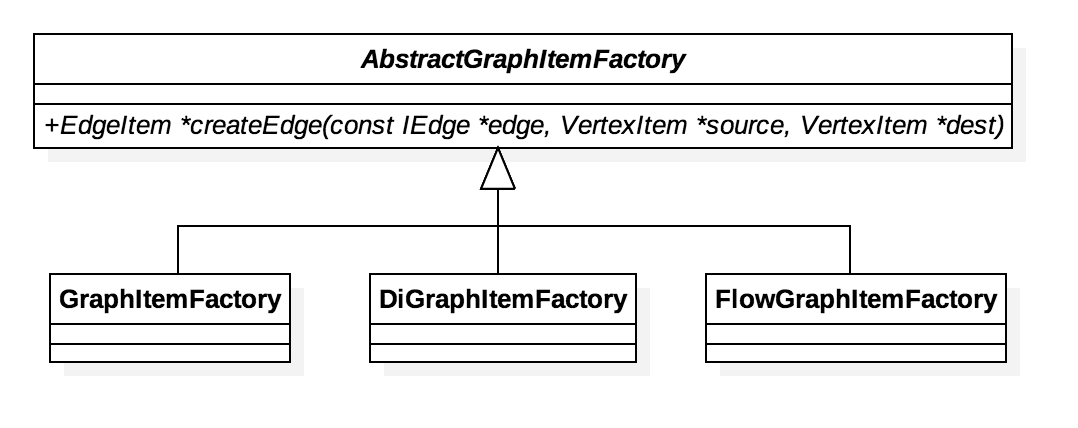
\includegraphics[width=0.6\textwidth]{Conception/visualization/graphitemsfactories.png}
		\caption{Diagramme de classes de la fabrication des éléments graphiques}
	\end{figure}
	
	Les factories sont donc toutes du même type de base, une classe abstraite qui définit les méthodes de création. Il y a ensuite une classe spécialisée par type de graphe, par famille (normal, dirigé et de flot). Ces sous-classes ont ensuite simplement à retourner une instance de l'élément graphique correspondant à ce type. \\
	
	Voici un exemple d'utilisation :
	
	\begin{lstlisting}
					// Surchage d'une methode de creation
					// pour retourner une instance de la famille
					EdgeItem *DiGraphItemFactory::createEdge(const IEdge *edge, VertexItem *source,
					VertexItem *dest)
					{
						return new DiEdgeItem(edge, source, dest);
					}
	\end{lstlisting}
	
	\begin{lstlisting}
					// Creation de la factory correspondante a la bonne famille
					AbstractGraphItemFactory *factory;
					if (dynamic_cast<const FlowGraph *>(graph)) {
						factory = new FlowGraphItemFactory();
					}
					else if (dynamic_cast<const DiGraph *>(graph)) {
						factory = new DiGraphItemFactory();
					}
					...
					
					// Creation d'un objet EdgeItem sans se soucier de son reel type
					EdgeItem *edgeItem = factory->createEdge(
						pointeurDeEdge,
						sommetSource,
						sommetDestination
					);
	\end{lstlisting}
	
	\pagebreak
	
	\subsection{Widget}
	Afin de simplifier l'affichage d'un graphe depuis la partie GUI, j'ai fait en sorte qu'un nouvel objet s'occupe d'instancier les objets nécessaires (vue et scène) et de configurer ces derniers. Il s'agit de la classe \textbf{GraphWidget} qui prend en paramètre un pointeur de IGraph à traiter. Ce widget peut ensuite être incorporé dans n'importe quelle layout, avec n'importe quelle dimension, sans se soucier du fonctionnement interne.
	
	\begin{figure}[H]
		\centering
		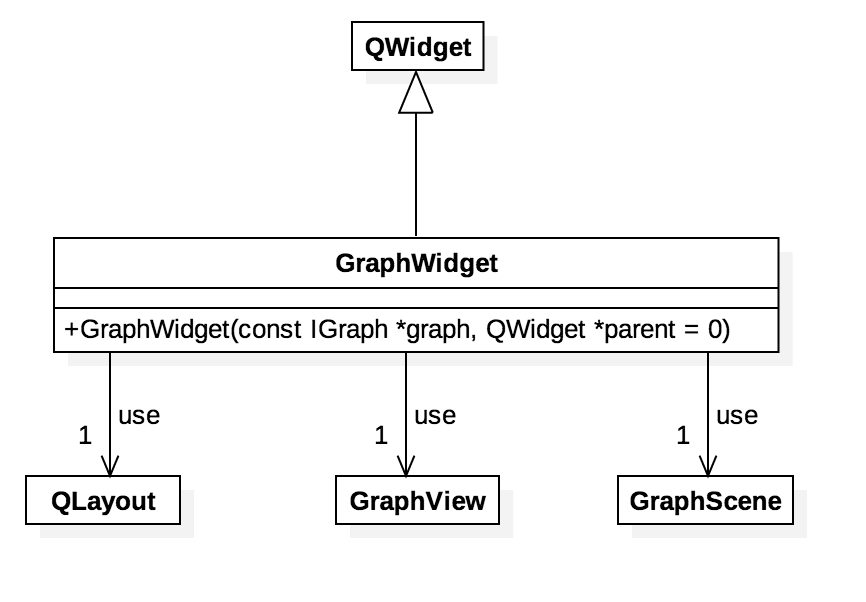
\includegraphics[width=0.6\textwidth]{Conception/visualization/graphwidget.png}
		\caption{Diagramme de la classe GraphWidget}
	\end{figure}
	
	Cette classe hérite de \textbf{QWidget}, une classe de Qt permettant jsutement d'être ajoutée et affichée dans un layout. Le widget possède également un layout, nécessaire pour y ajouter et afficher la vue du graphe.
	
	\subsection{Exportation}
	L'exportation des graphes (uniquement au format SVG pour ce projet) s'effectue à l'aide de la classe \textbf{GraphExporter}. Cette classe met à disposition des méthodes statiques permettant d'exporter au format SVG. \\
	Ces méthodes prennent un pointeur de IGraph en paramètre, elles génèrent ensuite la scène correspondante au graphe, puis l'enregistre dans un fichier.
	
	\begin{figure}[H]
		\centering
		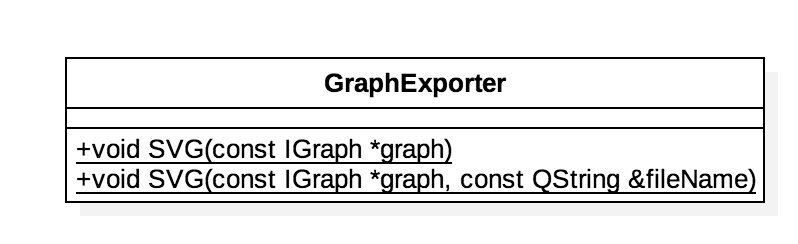
\includegraphics[width=0.4\textwidth]{Conception/visualization/graphexporter.png}
		\caption{Diagramme de la classe GraphExporter}
	\end{figure}
	
	Pour l'exportation SVG, il y a deux méthodes. Une avec un chemin de fichier en paramètre, l'autre sans. La méthode sans chemin va automatiquement ouvrir une fenêtre invitant l'utilisateur à choisir l'emplacement et le nom du fichier à enregistrer (à l'aide de la classe \textbf{QFileDialog} de Qt). Celle-ci va ensuite appeler la deuxième méthode avec le nom du fichier spécifié. \\
	Pour l'exportation, la scène est simplement rendue dans un objet spécifique à la place de celui gérant l'affichage. Il s'agit d'un objet \textbf{QSvgGenerator}. Ce dernier prend en paramètre le chemin du fichier et la taille du dessin SVG à créer. \\
	
	Le générateur s'utilise ensuite simplement en appelant l'une de ses méthodes statiques.
	
	\begin{lstlisting}
					GraphExporter::SVG(myGraph);
					// ou
					GraphExporter::SVG(myGraph, "/path/to/svg/file.svg");
	\end{lstlisting}
	
	\subsection{Réutilisation}
	Un problème se posait quant à la génération des graphes. Si un utilisateur affichait un graphe, déplaçait les sommets pour obtenir un affichage plus lisible et qu'il souhaitait ensuite l'exporter, le fichier contiendrait l'affichage par défaut (en grille actuellement) et pas ces modifications. Ceci représente également une perte de temps de régénérer l'affichage entier, alors que celui-ci a déjà été fait. \\
	Nous avons donc décidé d'implémenter un manageur de scènes (GraphScene) qui se charge de créer une nouvelle scène à partir d'un IGraph seulement si nécessaire. Ce manageur devait donc avoir connaissance des changements survenus sur les graphes. En clair, un graphe qui n'a pas changé (sommets, arêtes, etc.) doit utiliser la même scène d'un affichage à l'autre. \\
	
	Il n'était pas facile de mémoriser l'état des graphes. Nous avons donc créé une méthode de hashage d'un IGraph, prenant en compte tous les attributs des graphes. Le hash obtenu permet de distinguer un graphe avant et après une modification. Les scènes sont donc stockées par le manageur et liées à un hash. Lors de la demande de création d'une scène, les hashs sont comparés et s'il y a une concordance, la scène existante est retournée à la place qu'une nouvelle soit créée.
	
	\begin{figure}[H]
		\centering
		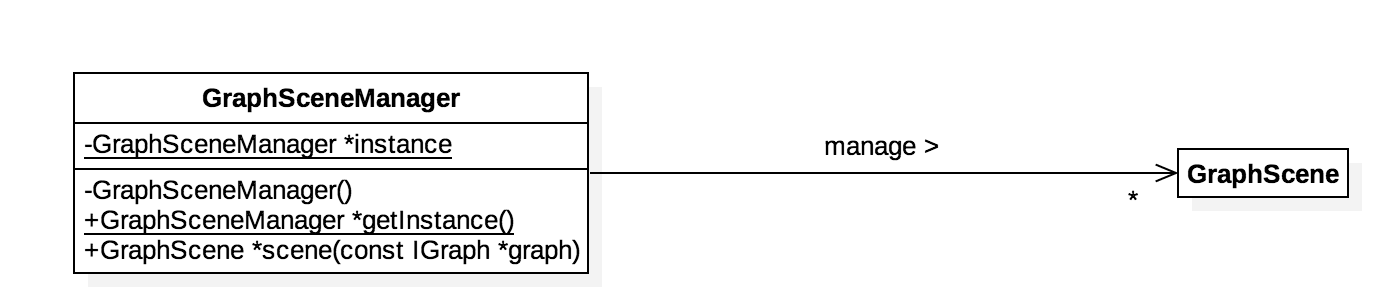
\includegraphics[width=0.8\textwidth]{Conception/visualization/graphscenemanager.png}
		\caption{Diagramme de la classe GraphSceneManager}
	\end{figure}
	
	Cela permet donc d'économiser du temps et permet aux utilisateurs de garder en mémoire les modifications qu'ils apportent visuellement aux graphes. \\
	
	Les objets désirant une instance de la classe GraphScene doivent donc maintenant toujours passer par le manageur.

	\section{Interpréteur} % Champion
		Dans le cadre de l'application, l'utilisateur est amené à entrer des commandes lui permettant de créer et de modifier des graphes, tout autant que d'appeler des fonctions effectuant différents traitements (algorithmes, lecture depuis un fichier, ...).\\
		
		Note: les détails d'implémentation peuvent être consultés dans l'annexe~\ref{sec:annexes-egli}.
	
		\subsection{Normalisation du langage} 
			Il est nécessaire de définir une grammaire claire sur la syntaxe des commandes, ainsi que leur sémantique.
			
			\subsubsection{Analyse des types et des opérations} 
			\label{subsubsec:analyse-des-types-et-des-operations}
				Premièrement, il faut définir les types disponibles dans le langage. Pour cela, il est intéressant de partir des algorithmes de graphe et de voir les types de résultats que nous attendons en sortie, ainsi que les types de paramètres dont nous aurons besoin:
			
				\begin{itemize}
					\item Boolean: un graphe a-t-il un cycle? est-il eulérien? ...
					\item Number: poids d'un arc, indice d'un sommet, ...
					\begin{itemize}
						\item Integer: pour les index, ...
						\item Float: pour les poids, ...
					\end{itemize}
					\item String: label d'un sommet, nom d'une fonction, ...
					\item Array: liste d'arêtes, matrices (Floyd-Warshall), ...
					\item Graph: le graphe à proprement parler
					\begin{itemize}
						\item Vertex: un sommet, son indice, son poids, ...
						\item Edge: une arête/arc, son poids, ...
					\end{itemize}
				\end{itemize} 
			
				Puisque nous avons à présent une idée des types disponibles, il faut définir leur domaine ainsi que les opérations disponibles et leur syntaxe. On fait le choix délibéré de se concentrer sur les opérations concernant les graphes, les opérations simples comme additionner deux nombres où les comparaisons ne sont pas prévues. Cependant la base du langage doit permettre de les définir plus tard. 
			
				\begin{longtable}{lll}
					\textbf{\texttt{Boolean}}\\ \hline \hline
					Domaine & \multicolumn{2}{l}{\texttt{True} ou \texttt{False}}\\ 
					Opérations & Déclaration & \texttt{Boolean a = True;}\\
					& Affectation & \texttt{a = False; a = f();}\\
					& Lecture & \texttt{a; f(a); Boolean b = a;}\\ 
					\\
					\textbf{\texttt{Number}}\\ \hline \hline
					Domaine & \multicolumn{2}{l}{\texttt{Integer} et \texttt{Float}}\\ 
					\\
					\textbf{\texttt{Integer}}\\ \hline \hline
					Domaine & \multicolumn{2}{l}{Entier signé sur 32 bits}\\
					Opérations & Déclaration & \texttt{Integer a = -20;}\\
					& Affectation & \texttt{a = 2; a = f();}\\
					& Lecture & \texttt{a; f(a); Integer b = a;}\\ 
					\\
					\textbf{\texttt{Float}}\\ \hline \hline
					Domaine & \multicolumn{2}{l}{Nombre à virgule flottante sur 32 bits}\\
					Opérations & Déclaration & \texttt{Float a = -32.4;}\\
					& Affectation & \texttt{a = 4.0; a = f();}\\
					& Lecture & \texttt{a; f(a); Float b = a;}\\ 
					\\
					\textbf{\texttt{String}}\\ \hline \hline
					Domaine & \multicolumn{2}{l}{Ensemble de zéros ou plusieurs caractères ASCII}\\
					Opérations & Déclaration & \texttt{String a = "Hello";}\\
					& Affectation & \texttt{a = "World"; a = f();}\\
					& Lecture & \texttt{a; f(a); String b = a;}\\ 
					\\
					\textbf{\texttt{Array}}\\ \hline \hline
					Domaine & \multicolumn{2}{l}{Tableau dynamique hétérogène}\\
					Opérations & Déclaration & \texttt{Array a = [1.0, "Salut", 3];}\\
					& Affectation & \texttt{a = [4, 5];}\\ 
					& Lecture & \texttt{a; f(a); Array b = a;}\\
					& Accès & \texttt{Integer c = a[1];}\\ 
					\\
					\textbf{\texttt{Vertex}}\\ \hline \hline
					Domaine & \multicolumn{2}{l}{Sommet avec des informations supplémentaires facultatives}\\
					Opérations & Déclaration & \texttt{Vertex a = (1); Vertex a2 = (2::3);}\\
					& & \texttt{(id:label:weight:max\_capacity:min\_capacity)}\\
					& Affectation & \texttt{a = (1:"Yverdon"); a = f();}\\
					& Lecture & \texttt{a; f(a); Vertex b = a;}\\ 
					\\
					\textbf{\texttt{Edge}}\\ \hline \hline
					Domaine & \multicolumn{2}{l}{Arête/arc avec des informations supplémentaires facultatives}\\
					Opérations & Déclaration & \texttt{Edge a = (1\textendash-2); Edge a2 = (2<-3:5);}\\
					& & \texttt{(connection[id]:weight:label:max\_capacity:min\_capacity)}\\
					& & \texttt{(arête: \textendash-, arcs: ->, <-)}\\
					& Affectation & \texttt{a = (1->2::"A1"); a = f();}\\
					& Lecture & \texttt{a; f(a); Vertex b = a;}\\ 
					\\
					\textbf{\texttt{Graph}}\\ \hline \hline
					Domaine & \multicolumn{2}{l}{Ensemble de sommets et d'arêtes/arcs}\\
					Opérations & Déclaration & \texttt{Graph a = \{0, 1, 2:A, 1->2:3:::2]\};}\\
					& & (si on ne veut pas écrire tous les sommets: \texttt{a = \{\#3, 0->1, 0->2\};})\\
					& & (les parenthèses pour les \texttt{Vertex} et \texttt{Edge} ne sont plus nécessaires)\\
					& Affectation & \texttt{a = \{0, 1, 0--1\}; a = f();}\\
					& Lecture & \texttt{a; f(a); Graph b = a;}\\
					& Ajout/modification & \texttt{a += (1<-2:4)};\\
					& Suppression & \texttt{a -= [(3), (1->2)];}\\
				\end{longtable}
				
				Ce tableau nous donne à présent une vue assez claire de nos besoins, cependant certaines opérations des types complexes (\texttt{Array, Vertex, Edge} et \texttt{Graph}) méritent d'être approfondies:
				
				\begin{itemize}
					\item \texttt{Array}: 
					\begin{itemize}
						\item Index de 0 à n-1
						\item Accès en dehors des bornes $\rightarrow$ Exception
					\end{itemize}
					\item \texttt{Vertex}:
					\begin{itemize}
						\item Seul le premier paramètre (\texttt{id[Integer]}) est obligatoire, et il ne doit pas être négatif (\texttt{id} est le nom, et entre \texttt{[]} c'est son type)
						\item Les valeurs par défaut sont \texttt{label[String]="", weight[Number]=0, max\_capacity[Number]=min\_capacity, min\_capacity[Number]=0}
					\end{itemize}
					\item \texttt{Edge}: 
					\begin{itemize}
						\item Seul le premier paramètre (\texttt{connection}) est obligatoire
						\item Le paramètre \texttt{id[Integer]} doit être positif ou nul et sa valeur par défaut est 0
						\item Les valeurs par défaut sont \texttt{weight[Number]=0, label[String]="", max\_capacity[Number]=min\_capacity, min\_capacity[Number]=0}
						\item L'\texttt{id} est un identifiant "local" à la \texttt{connection}, c'est-à-dire par exemple que \texttt{(0->1)} et \texttt{(1->0)} auront tous deux l'\texttt{id} à 0, et cela ne pose pas problème
					\end{itemize}
					\item \texttt{Graph}: 
					\begin{itemize}
						\item La création d'un graphe vide est permise (\texttt{Graph g = \{\};})
						\item Le raccourci d'écriture pour le nombre de sommets (\texttt{\#3}) doit se trouver au début
						\item Pour que le \texttt{Vertex} d'\texttt{id n} soit créé, il faut que tous les \texttt{id} de \texttt{0} à \texttt{n-1} existent déjà, sinon $\rightarrow$ Exception 
						\item Dans le cas d'arêtes/arcs multiples, par exemple \texttt{\{\#2, 0->1, 0->1\}}, le paramètre \texttt{id} du second \texttt{Edge} est incrémenté $\rightarrow$ \texttt{0->1[0]} et \texttt{0->1[1]}
						\item Pour qu'un \texttt{Edge} soit créé, il est nécessaire que les deux \texttt{Vertex} soient déjà créés, sinon $\rightarrow$ Exception
						\item Ajouts / modifications:
						\begin{itemize}
							\item Les types acceptés en opérande de droite sont \texttt{Vertex, Edge} ou un \texttt{Array} de ces deux types
							\item Pour les \texttt{Vertex}, si l'\texttt{id} existe déjà dans le graphe, c'est une modification, sinon c'est un ajout
							\item Pour les \texttt{Edge}, si la \texttt{connection} existe déjà dans le graphe mais que l'\texttt{id} est omis, alors c'est un ajout, sinon c'est une modification (sauf si l'\texttt{id} n'existe pas, dans ce cas c'est un ajout)
							\item La modification est cumulative, par exemple si on fait \texttt{Graph g = \{0:"Yverdon"\}; g += (0::2);}, alors le \texttt{Vertex} résultant est \texttt{(0:"Yverdon":2)}
						\end{itemize}
						\item Suppressions:
						\begin{itemize}
							\item Les types acceptés en opérande de droite sont \texttt{Vertex, Edge} ou un \texttt{Array} de ces deux types
							\item S'il n'y a rien à supprimer, alors il ne se passe rien (pas d'exception)
							\item La suppression d'un \texttt{Vertex} entraine la suppression des \texttt{Edge} associés
							\item Pour les \texttt{Edge}, si l'\texttt{id} est omis, alors toutes les \texttt{connection} sont supprimées
						\end{itemize}
					\end{itemize}
				\end{itemize}
				
				Notons que les erreurs sont gérées au travers d'exceptions.\\
				
				Maintenant que les types des variables et leurs opérations de base sont définis, on veut pouvoir effectuer d'autres traitements sur ces variables (ajouter une nouvelle opération ou appliquer un algorithme). Cela va se faire via des fonctions prédéfinies (la définition de fonctions n'est pas prévue).\\
				
				Prototype d'une fonction: \texttt{R f(T1, T2, ...);} avec \texttt{R} le type de retour, \texttt{f} le nom de la fonction et \texttt{Tn} le type du paramètre en position \texttt{n}.\\
				
				Appel d'une fonction: \texttt{Graph a = dijkstra(g, 1);} ou \texttt{g = removeAllPonderation(g);}.\\
				
				Le passage des paramètres se fait par copie (ou référence constante) et la correspondance est par position. On autorise la surcharge des fonctions.
			
		\subsection{Architecture}
			Un des buts de l'application est de pouvoir travailler sur plusieurs onglets en même temps. Cela implique que chacun aura des variables différentes et indépendantes.\\
			
			L'approche de base est que chaque onglet aura une instance de l'interpréteur:
			
			\begin{figure}[H]
				\centering
				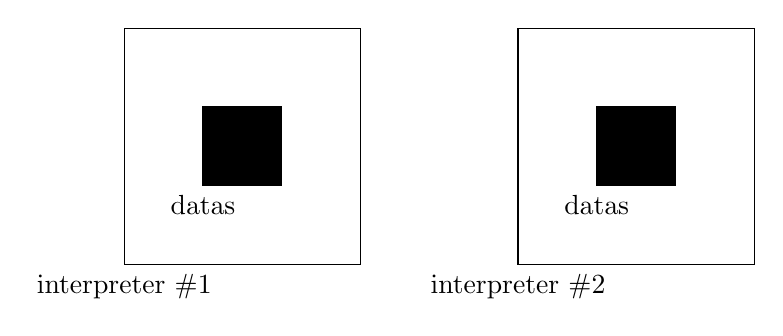
\begin{tikzpicture}
					\draw (0,0) node[anchor=north] {interpreter \#1} rectangle (3,3);
					\draw[fill=black] (1,1) node[anchor=north] {datas} rectangle (2,2);
					
					\draw (5,0) node[anchor=north] {interpreter \#2} rectangle (8,3);
					\draw[fill=black] (6,1) node[anchor=north] {datas} rectangle (7,2);
				\end{tikzpicture}
				\caption{Proposition d'architecture pour l'interpréteur}
			\end{figure}
			
			Cette approche a cependant le désavantage de dupliquer l'interpréteur dans la mémoire, alors que celui-ci est le même. Ce qui définit l'état dans lequel l'interpréteur est, c'est les données dans la mémoires virtuelle de celui-ci, c'est-à-dire la table des variables (voir éventuellement la table des fonctions). On peut donc développer une autre solution, très proche des processeurs et de leurs registres:
			
			\begin{figure}[H]
				\centering
				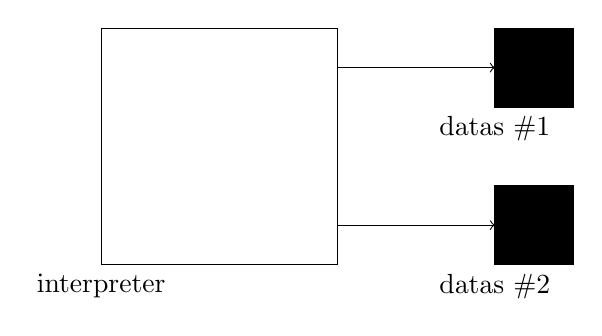
\begin{tikzpicture}
					\draw (0,0) node[anchor=north] {interpreter} rectangle (3,3);
					\draw[fill=black] (5,2) node[anchor=north] {datas \#1} rectangle (6,3);
					\draw[fill=black] (5,0) node[anchor=north] {datas \#2} rectangle (6,1);
					\draw[->] (3,2.5) -- (5,2.5);
					\draw[->] (3,0.5) -- (5,0.5);
				\end{tikzpicture}
				\caption{Architecture générale de l'interpréteur}
			\end{figure}
			
			A présent l'interpréteur n'est plus dupliqué, ainsi chaque onglet aura ses données et il suffira d'indiquer à l'interpréteur quel jeu de données il doit utiliser.
			
			\subsubsection{Interface utilisateur}
				Avant de s'attaquer au diagramme de classes, on peut se poser la question de l'interface qui sera fournie à l'utilisateur de l'interpréteur. Très simplement, celui-ci a besoin de:
				
				\begin{itemize}
					\item Instancier l'interpréteur
					\item Instancier une ou des tables des variables
					\item Connecter l'interpréteur à une table des variables
					\item Interfacer des fonctions avec l'interpréteur (éventuellement)
					\item Envoyer une commande (requête) à interpréter
					\item Récupérer le résultat d'une commande
					\item Connaître les fonctions disponibles
					\item Connaître les variables disponibles
				\end{itemize}
				
				Notons que les résultats peuvent être de plusieurs types: erreur avec message des détails, succès avec le nom de la variable de résultat.
			
			\subsubsection{Diagramme de classes}
			
				\begin{figure}[H]
					\centering
					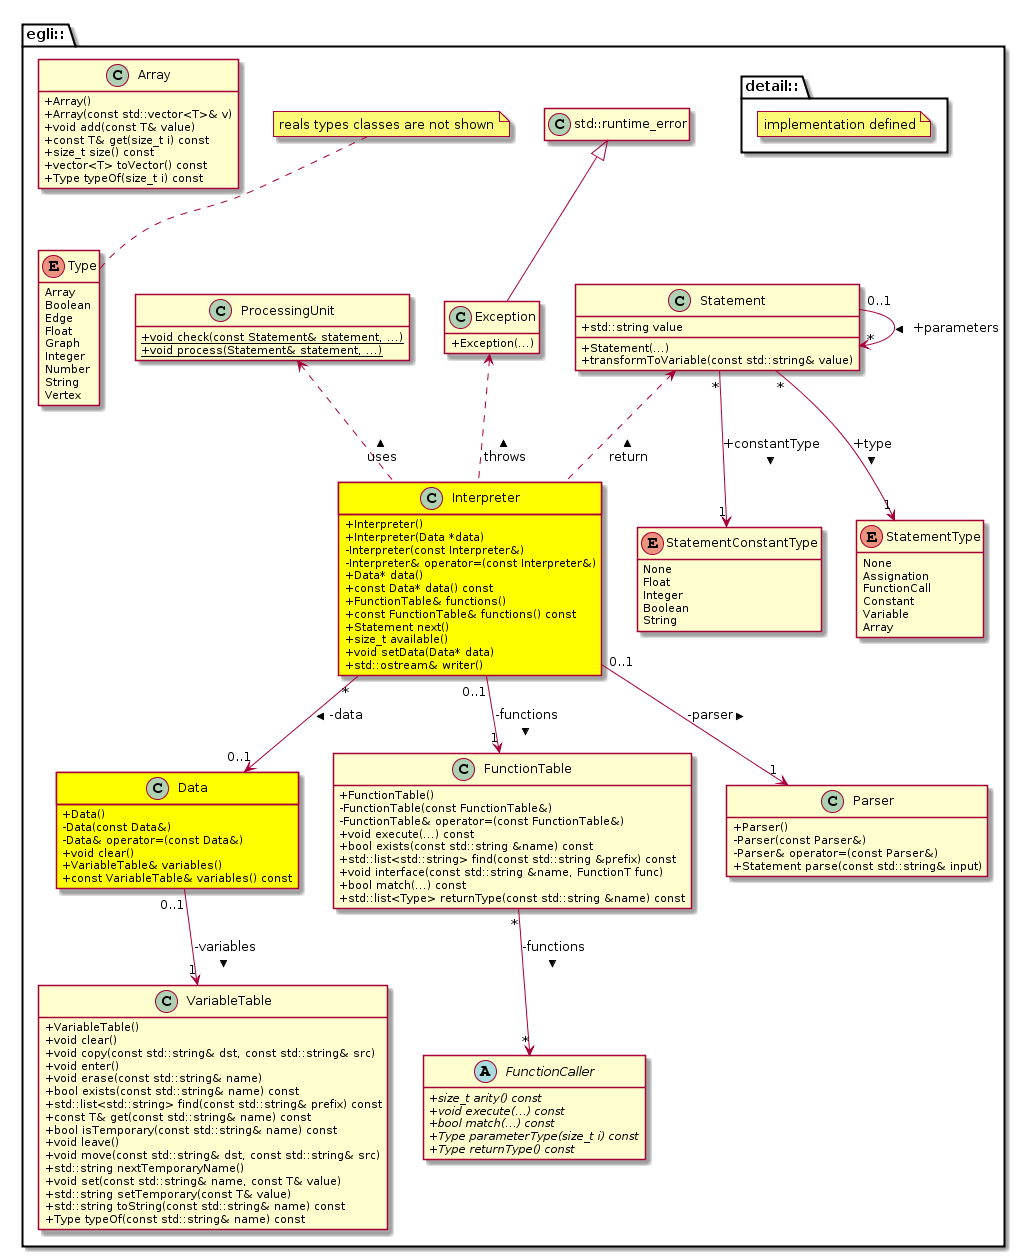
\includegraphics[width=\textwidth]{Conception/UMLEGLI}
					\caption{Diagramme de classes de l'interpréteur  \cite{plantuml}}
				\end{figure}
				
				Ce diagramme ne montre pas les attributs des classes car l'implémentation de chacune n'est pas fixée. De plus l'interface est là à titre indicative, il est possible qu'il y ait quelques modifications dans les sources. Pour finir certaines classes ont des $\dots$, cela indique que l'on ne sait pas encore à l'heure actuelle ce qu'il y aura à l'intérieur, ou que cela surchargerait trop le diagramme. Notons les classes surlignées en jaune vif, il s'agit des classes principales pour l'utilisateur (voir section~\ref{subsec:egli-exemple}).  
			
			\subsubsection{Répertoires}
				L'interpréteur étant une couche indépendante de l'application GUI, nous avons décidé de mettre tout ce qui le concerne dans un \texttt{namespace} du nom de \texttt{egli}, pour \textit{Embeeded GraphY Language Interpreter}.\\
				
				Voici à quoi ressemblera le répertoire de l'interpréteur:
				
				\begin{figure}[H]
					\centering
					\dirtree{%
						.1 egli/\DTcomment{répertoire de base de EGLI}.
						.2 detail/\DTcomment{répertoire "privé", ne doit pas être utilisé par l'utilisateur}.
						.3 interface/\DTcomment{répertoire pour les fonctions interfacées}.
						.4 algorithms.h\DTcomment{les algorithmes venant des couches \textit{graphes et algorithmes}}.
						.4 basics.h\DTcomment{les fonctions nécessaires au fonctionnement interne}.
						.4 builtins.h\DTcomment{les fonctions offertes de base dans l'interpréteur}.
						.3 FunctionImpl.h\DTcomment{implémentation de \texttt{FunctionCaller}}.
						.3 Grammar.h\DTcomment{grammaire utilisée par le parseur}.
						.3 interface.h\DTcomment{interfaçage centralisé des fonctions}.
						.3 <...>\DTcomment{autres fichiers d'implémentation}.
						.2 Array.h\DTcomment{tableau dynamique hétérogène}.
						.2 Data.h\DTcomment{données utilisées dans l'interpréteur}.
						.2 egli.h\DTcomment{fichier d'inclusion générale}.
						.2 Exception.h\DTcomment{exception spécifique à EGLI}.
						.2 Function.h\DTcomment{déclaration de \texttt{FunctionCaller}}.
						.2 FunctionTable.h\DTcomment{table des fonctions}.
						.2 GraphWrapper.h\DTcomment{\textit{wrapper} de \texttt{IGraph} venant des couches \textit{graphes et algorithmes}}.
						.2 Interpreter.h\DTcomment{interpréteur de EGLI}.
						.2 Parser.h\DTcomment{parseur utilisé par l'interpréteur}.
						.2 ProcessingUnit.h\DTcomment{unité de vérification et de traitement}.
						.2 serialize.h\DTcomment{(dé-)sérialisation de \texttt{Data}}.
						.2 Statement.h\DTcomment{type de traitement possible}.
						.2 toString.h\DTcomment{transforme une variable en \texttt{std::string}}.
						.2 VariableTable.h\DTcomment{table des variables}.
						.2 <...>\DTcomment{autres fichiers}.
					}
				\end{figure}
			
		\subsection{Exemple}
		\label{subsec:egli-exemple}
			Dans cette section, nous allons voir un exemple d'utilisation de EGLI. Un code valant plus qu'un long discours, voici une utilisation en console qui prend les commandes en entrée et qui affiche les sorties correspondantes. On y voit également un exemple d'interfaçage d'une fonction.
			
			\begin{lstlisting}
					// main.cpp
					// Exemple d'utilisation de EGLI
					
					#include <iostream>
					#include <string>
					#include <cstdlib>
					#include <ctime>
					
					// Fichier d'inculsion de EGLI
					#include "egli/egli.h"
					
					using namespace std;
					
					// Fonction que l'on souhaite interfacer
					int random(int min, int max)
					{
						return min + rand() / (RAND_MAX / (max - min + 1) + 1);
					}
					
					int main()
					{
						srand(time(nullptr));
						
						// On cree l'interpreteur
						egli::Interpreter interpreter;
						
						// On interface notre fonction
						interpreter.functions().interface("rand", random);
						
						// On a besoin de donnees sur lesquelles travailler
						egli::Data data;
						
						// On indique a l'interpreteur quelles donnees il doit utiliser
						interpreter.setData(&data);
						
						// On lit l'entree utilisateur
						string input;
						while (getline(cin, input)) {
						
							// On quitte si input == "q"
							if (input == "q")
								break;
							
							// On ecrit l'entree dans l'interpreteur
							// (writer() retourne un std::ostream&)
							interpreter.writer() << input;
							
							// Tant que des commandes sont disponibles
							while (interpreter.available()) {
								try {
								
									// On execute la commande en recuperant son resultat
									// (statement.value contiendra le nom de la variable generee)
									egli::Statement statement = interpreter.next();
									
									// On verifie si la variable existe
									// (elle n'existe pas dans le cas ou c'etait une variable temporaire)
									if (data.variables().exists(statement.value)) {
									
										// Elle existe! On affiche sa valeur
										string value = data.variables().toString(statement.value);
										string type = egli::toString(data.variables().typeOf(statement.value));
										if (value.size() > 50) { // mise en page
											value.resize(50);
											value.append("...");
										}
										cout << ">> " << statement.value << " (" << type << ") <- " << value 
										     << endl;
									}
									else
										cout << ">> temporary returned" << endl;
								
								// Les erreurs sont gerees grace aux exceptions
								} catch(const exception &ex) {
									cout << ex.what() << endl;
								}
							}
							
							cout << endl; // mise en page
						}
						
						// Fin
						return 0;
					}
			\end{lstlisting}
			
			\subsubsection{Fonctions incluses}
			\label{subsec:annexes-fonctions-incluses}
			Cette section recense les fonctions incluses dans l'interpréteur et disponibles pour l'utilisateur de l'application. Les fonctions \textit{built-in} viennent de l'interpréteur directement, les fonctions \textit{algo} proviennent de la couche sur les graphes et ses algorithmes, et les fonctions \texttt{GUI} sont spécifiques à la couche interface utilisateur.\\
			
			Note: les paramètres de type \texttt{T} indiquent qu'il existe une surcharge de la fonction pour chacun des types disponible dans le langage.
			
			\begin{figure}[H]
				\centering
				\begin{longtable}{p{0.45\textwidth}p{0.45\textwidth}p{0.1\textwidth}}
					Prototype & Description & Origine\\
					\hline
					\texttt{String toString(T a)} & Retourne la représentation de \texttt{a} sous forme de chaîne & \textit{built-in}\\
					\texttt{Boolean save(Graph g, String file)} & Sauvegarde le graphe \texttt{g} dans le fichier \texttt{file} & \textit{built-in}\\
					\texttt{Graph load(String file)} & Charge le graphe contenu dans le fichier \texttt{file} & \textit{built-in}\\
					\texttt{String typeOf(T a)} & Retourne le type de \texttt{a} sous forme de chaîne & \textit{built-in}\\
					\texttt{Graph er(Integer V, Float p)} & Génère un graphe aléatoire à \texttt{V} sommets et une probabilité d'inclusion des arêtes de \texttt{p} & \textit{built-in} \\
					
					\texttt{Boolean draw(Graph g)} & Dessine le graphe \texttt{g} & \textit{GUI}\\
					\texttt{Boolean exportAsSvg(Graph g)} & Exporte le graphe \texttt{g} en SVG & \textit{GUI}\\
					\texttt{Boolean exportAsSvg(Graph g, String file)} & Exporte le graphe \texttt{g} en SVG dans le fichier \texttt{file} & \textit{GUI}\\
					
					\texttt{Array bellmanFord(Graph g, Integer from)} & Applique un Bellman-Ford au graphe \texttt{g} depuis le sommet \texttt{from} & \textit{algo}\\
					\texttt{Array bfs(Graph g, Integer from)} & Applique un BFS sur le graphe \texttt{g} depuis le sommet \texttt{from} & \textit{algo}\\
					\texttt{Array cc(Graph g)} & Cherche les composantes connexes du graphe \texttt{g} & \textit{algo}\\
					\texttt{Graph detectCycle(Graph g)} & Retourne un cycle du graphe \texttt{g}, si il y en a un & \textit{algo}\\
					\texttt{Array dfs(Graph g, Integer from)} & Applique un DFS sur le graphe \texttt{g} depuis le sommet \texttt{from} & \textit{algo}\\
					\texttt{Array dijkstra(Graph g, Integer from)} & Applique un Dijkstra au graphe \texttt{g} depuis le sommet \texttt{from} & \textit{algo}\\
					\texttt{Boolean isConnected(Graph g)} & Vérifie si le graphe \texttt{g} est connexe & \textit{algo}\\
					\texttt{Boolean isDirected(Graph g)} & Vérifie si le graphe \texttt{g} est orienté & \textit{algo}\\
					\texttt{Boolean isEmpty(Graph g)} & Vérifie si le graphe \texttt{g} est vide & \textit{algo}\\
					\texttt{Boolean isNegativeWeighted(Graph g)} & Vérifie si le graphe \texttt{g} possède des poids négatifs & \textit{algo}\\
					\texttt{Boolean isNull(Graph g)} & Vérifie si le graphe \texttt{g} est nul & \textit{algo}\\
					\texttt{Boolean isPlanar(Graph g)} & Vérifie si le graphe \texttt{g} est planaire & \textit{algo}\\
					\texttt{Boolean isSimple(Graph g)} & Vérifie si le graphe \texttt{g} est simple & \textit{algo}\\
					\texttt{Boolean isStronglyConnected(Graph g)} & Vérifie si le graphe \texttt{g} est fortement connexe & \textit{algo}\\
					\texttt{Boolean isWeighted(Graph g)} & Vérifie si le graphe \texttt{g} est pondéré & \textit{algo}\\
					\texttt{Graph kruskal(Graph g)} & Applique un Kruskal au graphe \texttt{g} & \textit{algo}\\
					%\texttt{Graph prim(Graph g)} & Applique un Prim au graphe \texttt{g} & \textit{algo}\\
					%\texttt{Graph prim(Graph g, Integer from)} & Applique un Prim au graphe \texttt{g} depuis le sommet \texttt{from} & \textit{algo}\\
					\texttt{Array tarjan(Graph g)} & Applique un Tarjan au graphe \texttt{g} & \textit{algo}\\
					\texttt{Array topologicalSort(Graph g)} & Applique un tri topologique au graphe \texttt{g} & \textit{algo}\\
				\end{longtable}
			\end{figure}
		
	\section{Graphes}
	\label{sec:graphes}
		\subsection{Préface}
		Un graphe est une structure composée d'un ensemble de sommets et d'arêtes/arcs. Il existe différents moyens de les représenter.
		
		Cette section a pour but de présenter les interfaces à disposition de l'utilisateur pour manipuler des graphes, ainsi que de montrer nos choix de modélisation et d'implémentation de ceux-ci.
		
		\subsection{Architecture}
		
			\subsubsection{Diagramme de classe}
			\begin{figure}[H]
				\centering
				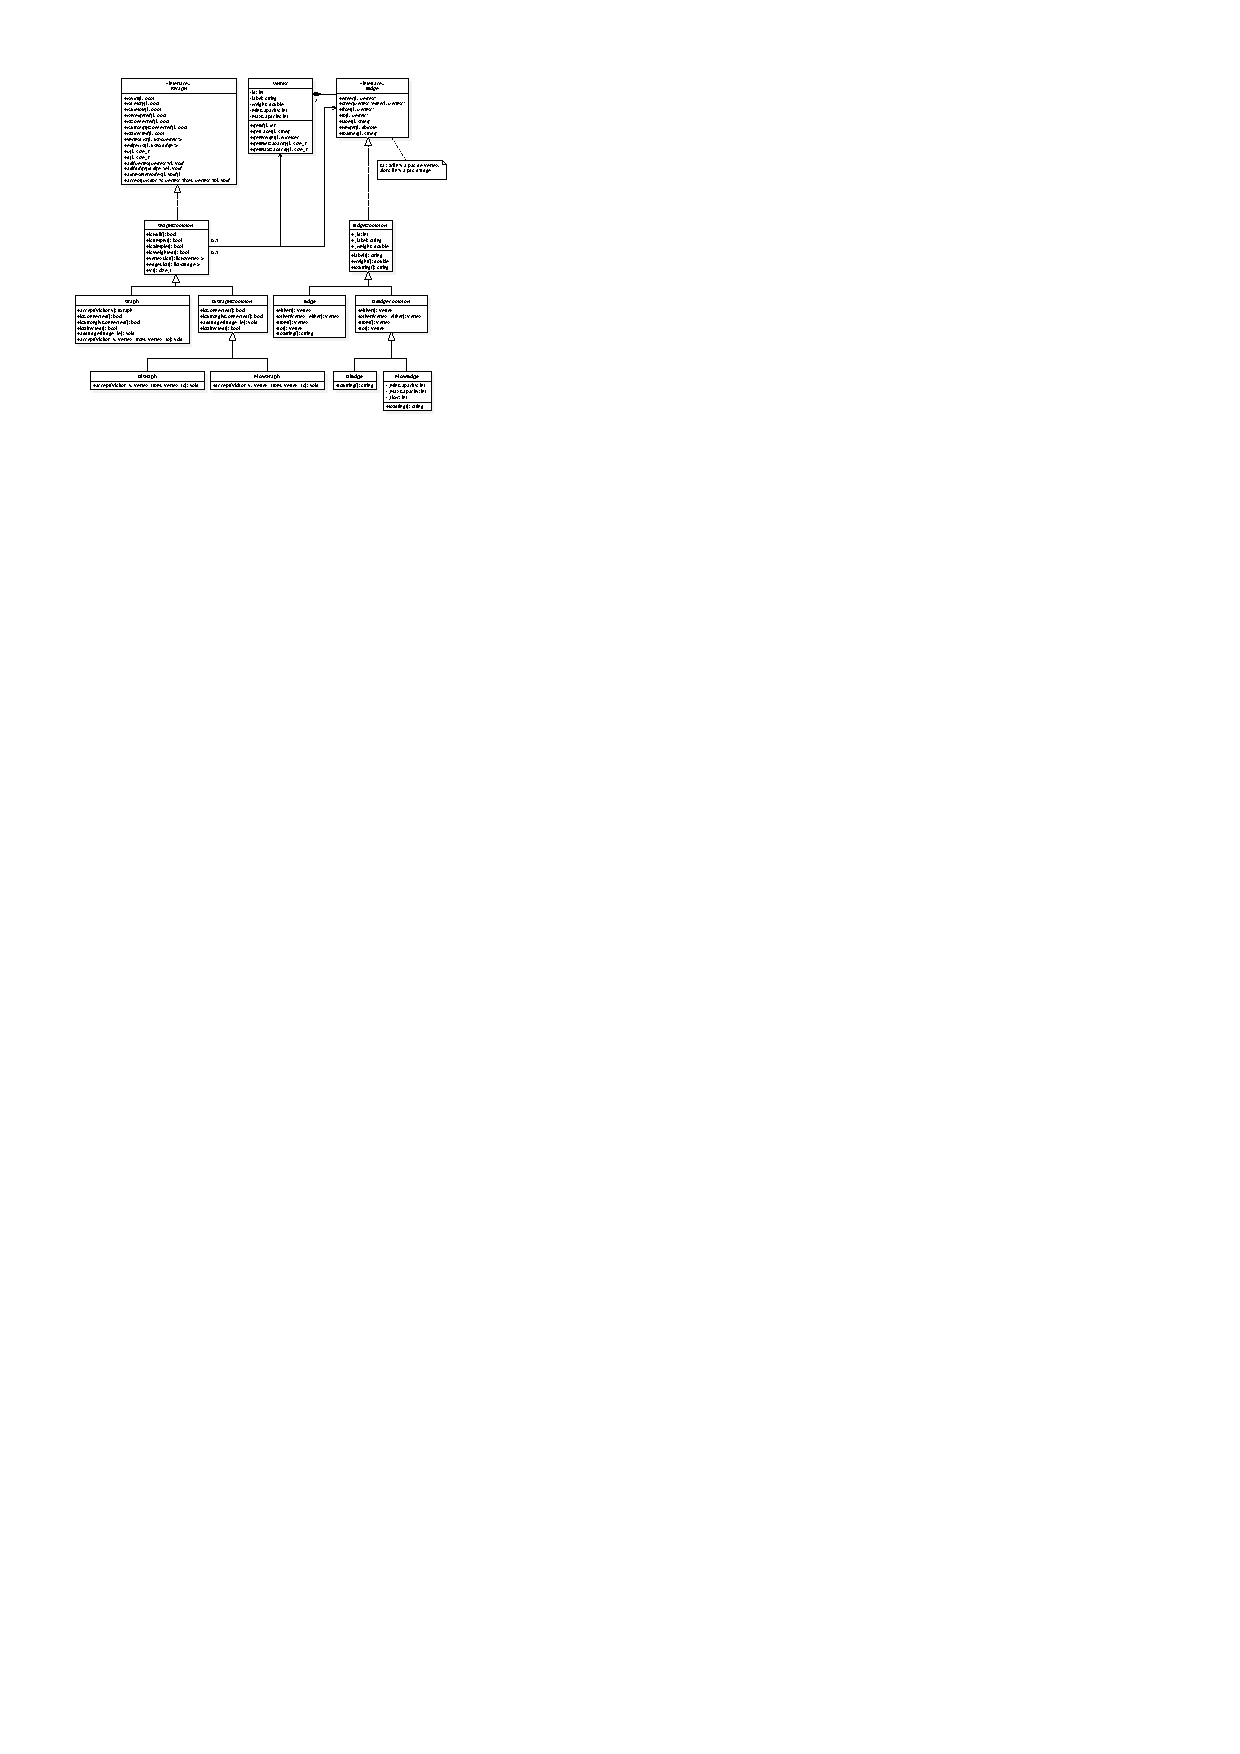
\includegraphics[scale=2.8]{Conception/graph/umlGraph.pdf}
				\caption{Diagramme de classe pour les graphes}
			\end{figure}
		
			\subsubsection{La classe "Vertex"}
			Les sommets sont les mêmes pour tous les types de graphe (orienté, à flot, ou non-orienté). Les informations suivantes y sont stockées :
			\begin{itemize}
				\item un identifiant géré par la classe "Graph" ci-après
				\item un label pour spécifier un nom au sommet
				\item un poids de type numérique qui pourra être ensuite redistribué sur les arêtes par exemple
				\item une capacité minimale de type numérique entière
				\item une capacité maximale de type numérique entière 
			\end{itemize}
			Voici un aperçu des attributs de la classe en question
			\begin{lstlisting}
						// Apercu de la classe Vertex
						public class Vertex {
							private:
								int _id;
								string _label;
								double _weight;
								int _minCapacity;
								int _maxCapacity;
								
							public:
								// Constructeur vide. Valeurs par defaut.
								Vertex() : _id(-1), _label(""), _weight(numeric_limits<double>::max()),
											_minCapacity(-1), _maxCapacity(-1) {}
								// setter et getter...
								// ...
						};
			\end{lstlisting}
			Les capacités sont des entiers signés uniquement pour leur donner une valeur par défaut de -1. On aurait pu les déclarer avec un type non-signé mais nous trouvions plus léger au niveau du code de le faire de cette manière.
			
			\subsubsection{La classe "Edge"}
			Les arcs/arêtes sont plus délicats car ils diffèrent entre les types de graphe. Les trois types présents dans l'application sont les suivants :
			\begin{itemize}
				\item arête, type \lstinline[basicstyle=\ttfamily\color{blue}]|Edge|
				\item arc, type \lstinline[basicstyle=\ttfamily\color{blue}]|DiEdge| pour Directed Edge
				\item arc à flot, type \lstinline[basicstyle=\ttfamily\color{blue}]|FlowEdge|\\
			\end{itemize}
			
			Les attributs communs aux trois types sont :
			\begin{itemize}
				\item un id pour identifier l'Edge de façon unique au sein d'un graphe donné
				\item un pointeur sur le sommet source nommé $a$
				\item un pointeur sur le sommet destination nommé $b$
				\item un label pour nommer l'Edge
				\item un poids de type numérique pour lui associer un poids
				\item En plus pour les \lstinline[basicstyle=\ttfamily\color{blue}]|FlowEdge| : une capacité minimum de type numérique entière
				\item En plus pour les \lstinline[basicstyle=\ttfamily\color{blue}]|FlowEdge| : une capacité maximum de type numérique entière
				\item En plus pour les \lstinline[basicstyle=\ttfamily\color{blue}]|FlowEdge| : le flot courant de type numérique entier\\
			\end{itemize}
			
			Notons que pour un \lstinline[basicstyle=\ttfamily\color{blue}]|Edge|, les sommets $a$ et $b$ ne font pas office de "source" et "destination" puisque l'arc n'est pas orienté.\\
			
			Nous sommes donc partis sur une première approche qui consiste à avoir une classe Edge commune dont les Edge spécifiques hériteront selon le type de graphe.
			\begin{figure}[H]
				\centering
				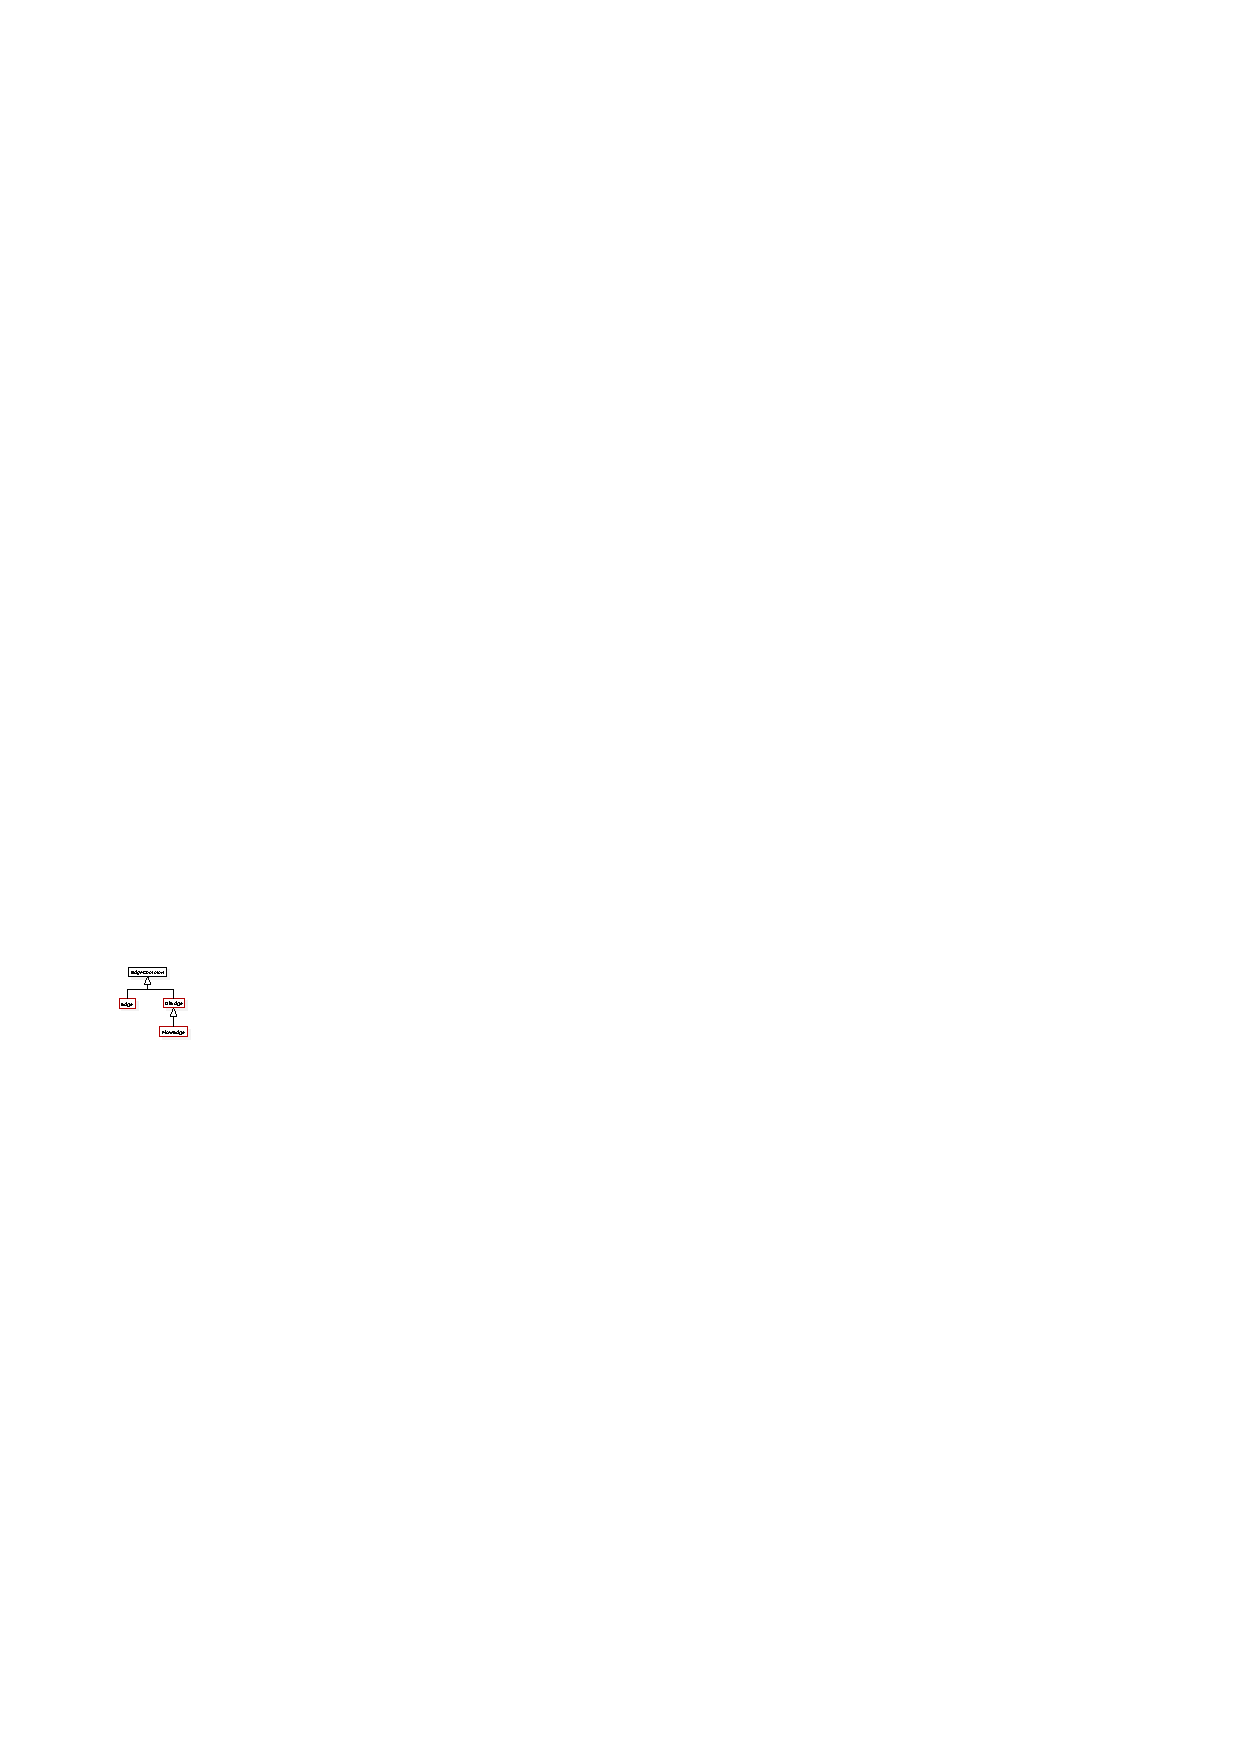
\includegraphics[scale=4.0]{Conception/graph/classedgesol1.pdf}
				\caption{Classe Edge solution 1}
			\end{figure}
			Cette approche est optimale car elle permet une bonne factorisation du code. Seulement, nous avons rencontré un problème lors de la mise en place de la classe Graph où les types de Edge sont passés par template (expliqué dans le chapitre "classe Graph"). Avec la solution ci-dessus nous n'avons pas trouvé le moyen de spécifier explicitement le type \lstinline[basicstyle=\ttfamily\color{blue}]|FlowEdge| au graphe sans générer d'erreur de compilation : \lstinline[basicstyle=\ttfamily\color{blue}]|FlowEdge| étant un sous-type de \lstinline[basicstyle=\ttfamily\color{blue}]|DiEdge|, le compilateur ne parvenait pas à faire le lien sur le bon type. Nous nous sommes donc résiliés à modifier l'architecture de la classe "Edge" pour n'avoir que des types distincts.
			\begin{figure}[H]
				\centering
				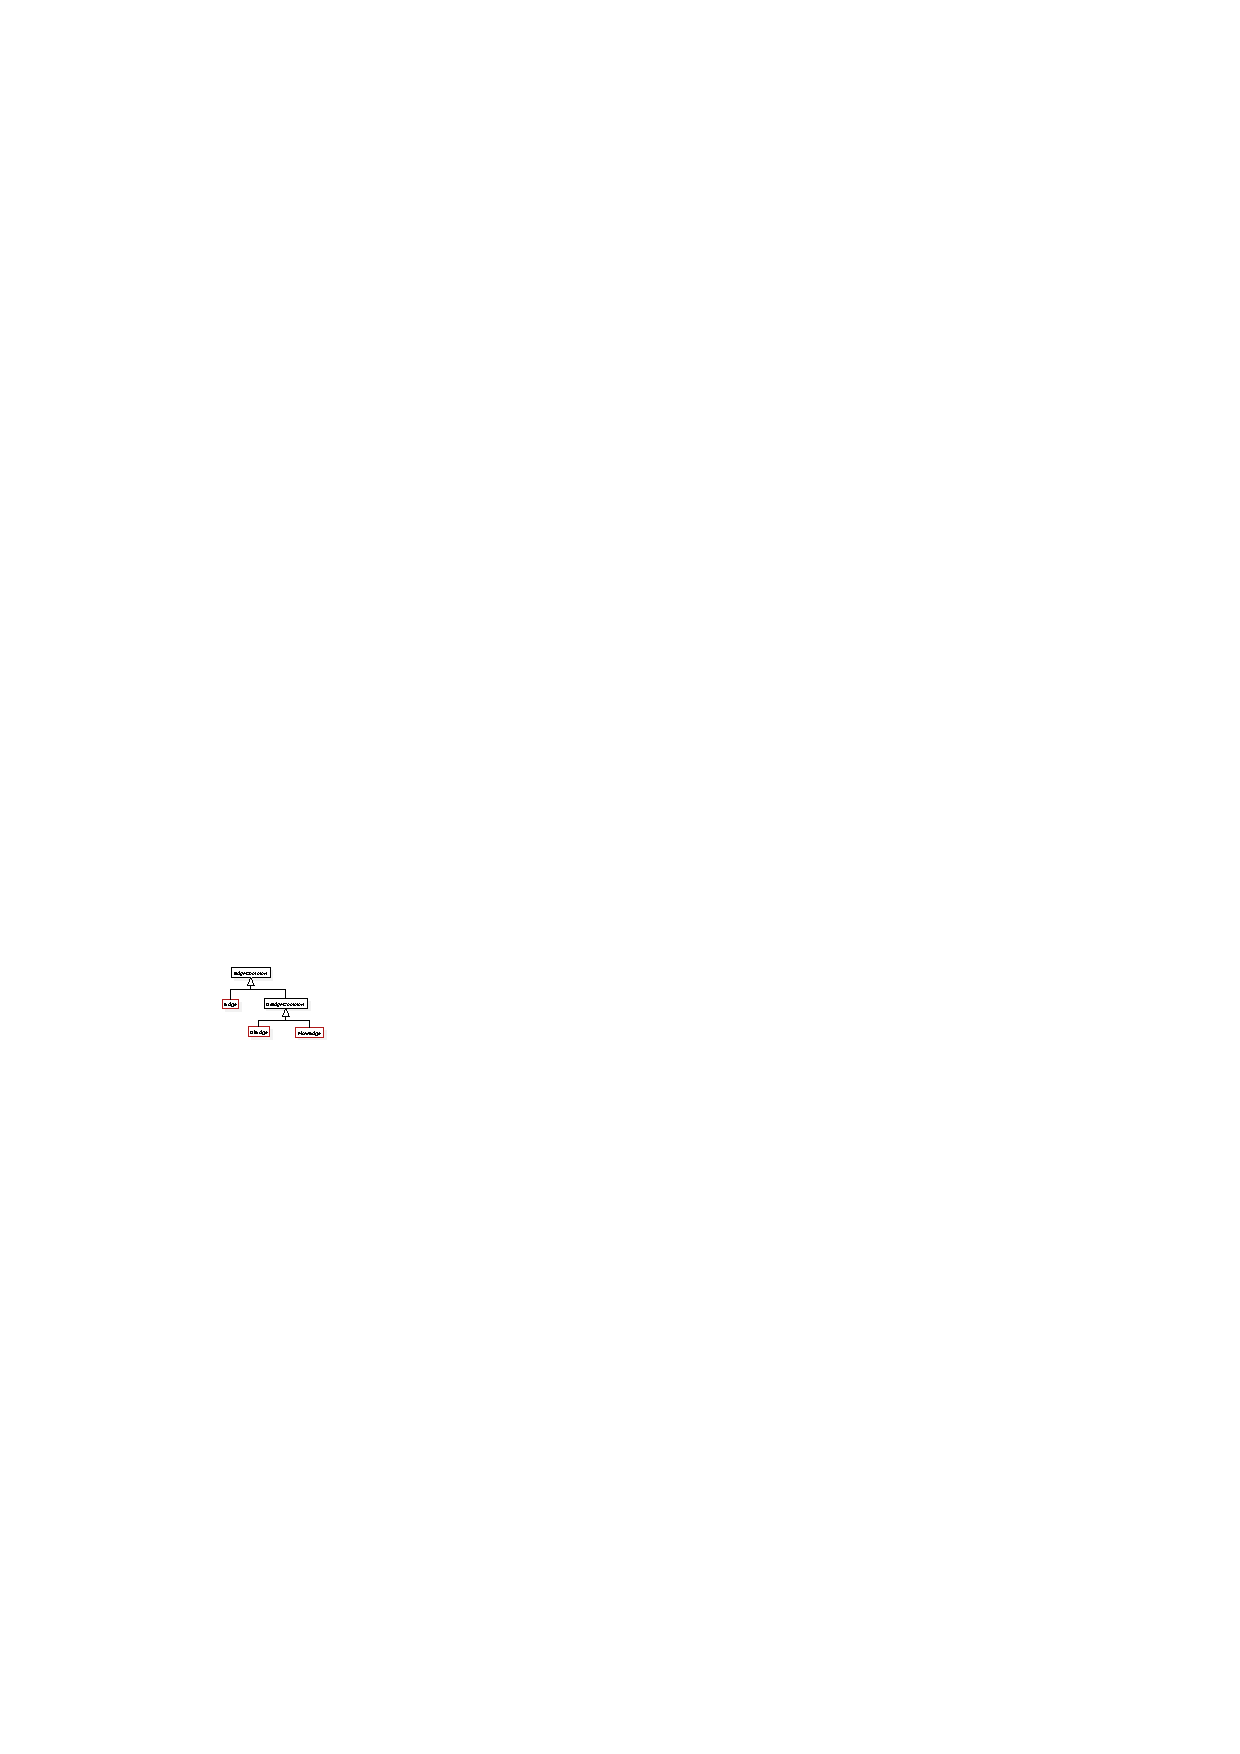
\includegraphics[scale=4.0]{Conception/graph/classedgesol2.pdf}
				\caption{Classe Edge solution 2}
			\end{figure}
			
			Une interface \lstinline[basicstyle=\ttfamily\color{blue}]|IEdge| est ensuite ajoutée pour fournir à l'utilisateur un moyen unique de manipuler tout type de Edge.
			\begin{figure}[H]
				\centering
				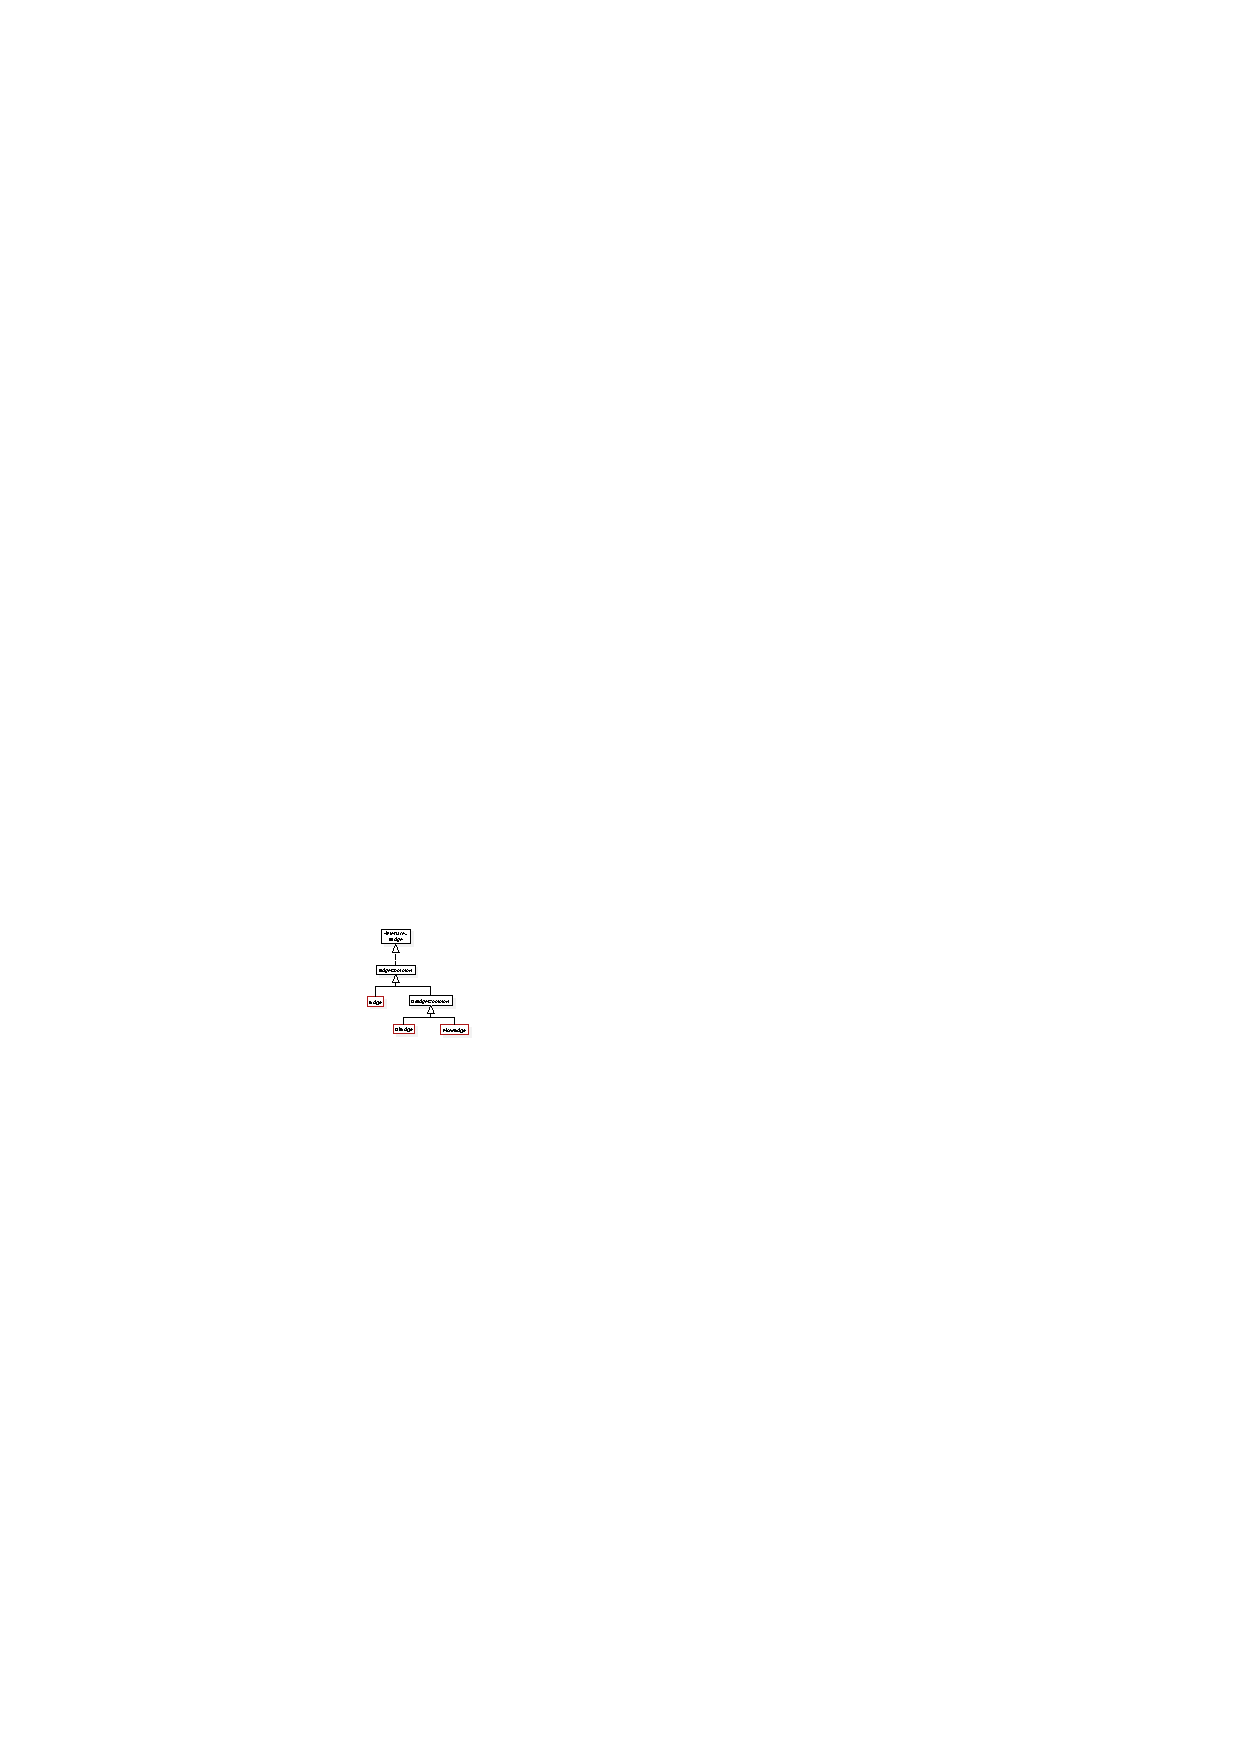
\includegraphics[scale=4.0]{Conception/graph/classedgesol3.pdf}
				\caption{Classe Edge solution finale}
			\end{figure}
			
			Ainsi, grâce à la covariance des variables, l'utilisateur peut voir n'importe quel type de Edge en tant qu'IEdge et le manipuler de la sorte.
			\begin{lstlisting}
						// Edge entre le sommet v1 et v2
						IEdge *edge = new Edge(v1, v2, 4.5);
						
						// DiEdge du sommet v1 au sommet v2
						IEdge *diEdge = new DiEdge(v1, v2, 6.0);
						
						// FlowEdge de capacite 3 du sommet v1 au sommet v2
						IEdge *flowEdge = new FlowEdge(v1, v2, 5.2, 3);
						
						// exemple de methode
						cout << edge->weight() << endl; // Affiche 4.5
						cout << diEdge->weight() << endl; // Affiche 6
						cout << flowEdge->weight() << endl; // Affiche 5.2
			\end{lstlisting}
						
			\subsubsection{Classe "Graph"}
			Cette classe est étroitement liée à la classe "Edge". Sachant qu'il existe trois types d'Edge, il existe donc 3 types de graphe :
			\begin{itemize}
				\item Graphe non-orienté
				\item Graphe orienté
				\item Graphe orienté à flot
			\end{itemize}
			Nous gardons la même architecture que la classe "Edge". Les trois types doivent être distincts (un graphe à flot ne doit pas hériter directement d'un graphe orienté) pour expliciter clairement le type de Edge.
			Une première approche nous avait mené à déclarer les classes "Edge" internes aux classes "Graph" correspondantes mais cette méthode s'est avérée trop complexe. Une deuxième approche consistait plutôt à passer le type de Edge en template à la classe Graph correspondante. Cette deuxième approche nous paraissait plus simple et nous avons donc opté pour celle-ci.
			Voici à quoi ressemble le modèle conceptuel de la classe "Graph".
			\begin{figure}[H]
				\centering
				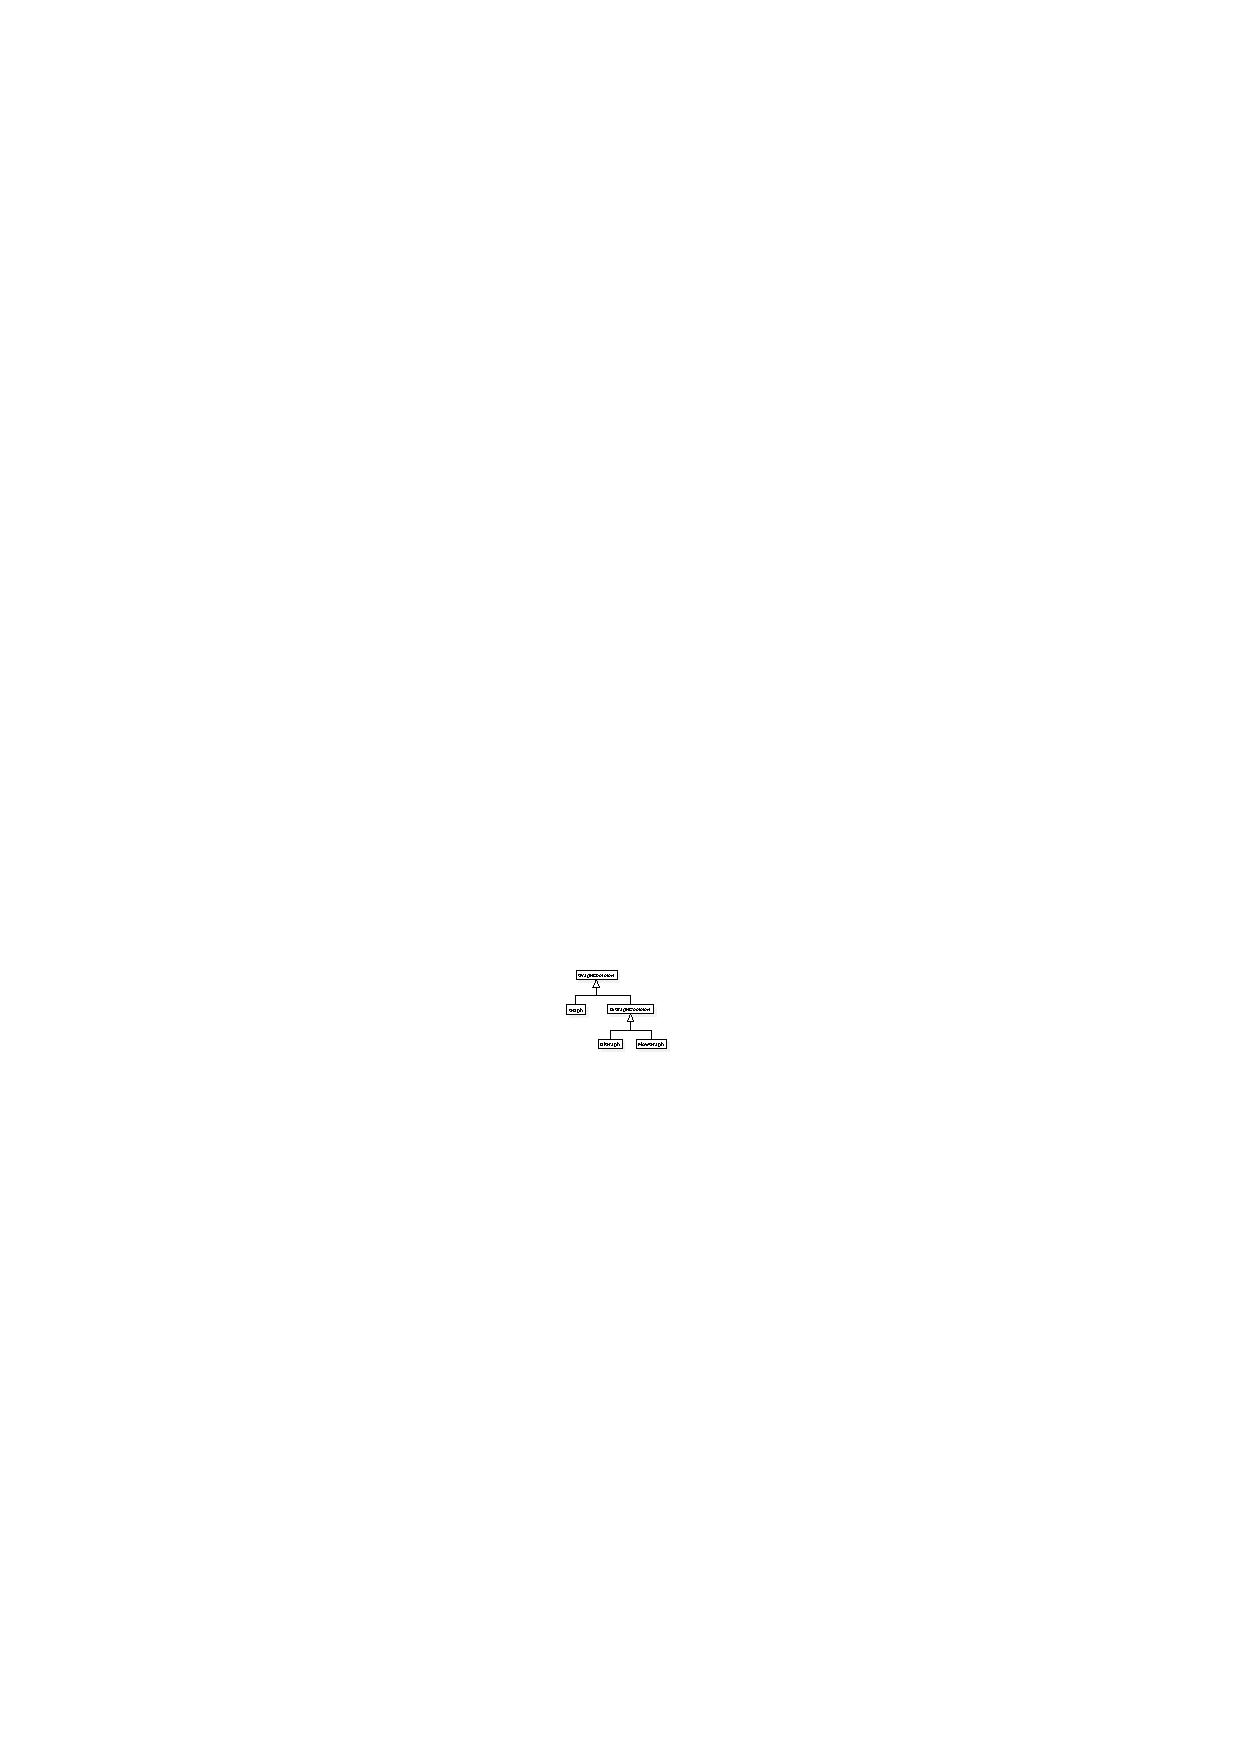
\includegraphics[scale=4.0]{Conception/graph/classgraphsol1.pdf}
				\caption{Classe Graph solution finale}
			\end{figure}
			Et voici comment expliciter le type de Edge avec les templates.
			\begin{lstlisting}
						template <typename T>
						class GraphCommon {
							//...
						}
						
						template <typename T>
						class DiGraphCommon : public GraphCommon<T> {
							//...
						}
						
						class Graph : public GraphCommon<Edge> {
							//...
						}
						
						class DiGraph : public DiGraphCommon<DiEdge> {
							//...
						}
						
						class FlowGraph : public GraphCommon<FlowEdge> {
							//...
						}
			\end{lstlisting}
			Ainsi, \lstinline[basicstyle=\ttfamily\color{blue}]|Graph| contient des \lstinline[basicstyle=\ttfamily\color{blue}]|Edge|, \lstinline[basicstyle=\ttfamily\color{blue}]|DiGraph| contient des \lstinline[basicstyle=\ttfamily\color{blue}]|DiEdge|, et \lstinline[basicstyle=\ttfamily\color{blue}]|FlowGraph| contient des \lstinline[basicstyle=\ttfamily\color{blue}]|FlowEdge|. Lors d'un appel à une méthode implémentée dans \lstinline[basicstyle=\ttfamily\color{blue}]|GraphCommon| qui traite des \lstinline[basicstyle=\ttfamily\color{blue}]|IEdge|, la méthode effectuera le lien sur le bon type de Edge au travers de la liaison dynamique.
		
			Pour abstraire tout ce contenu à l'utilisateur, une interface lui permettant la manipulation de tout type de graphes est créée au-dessus de l'architecture actuelle.
			Voici une ébauche de cette interface permettant la manipulation de graphes :
			\begin{figure}[H]
				\centering
				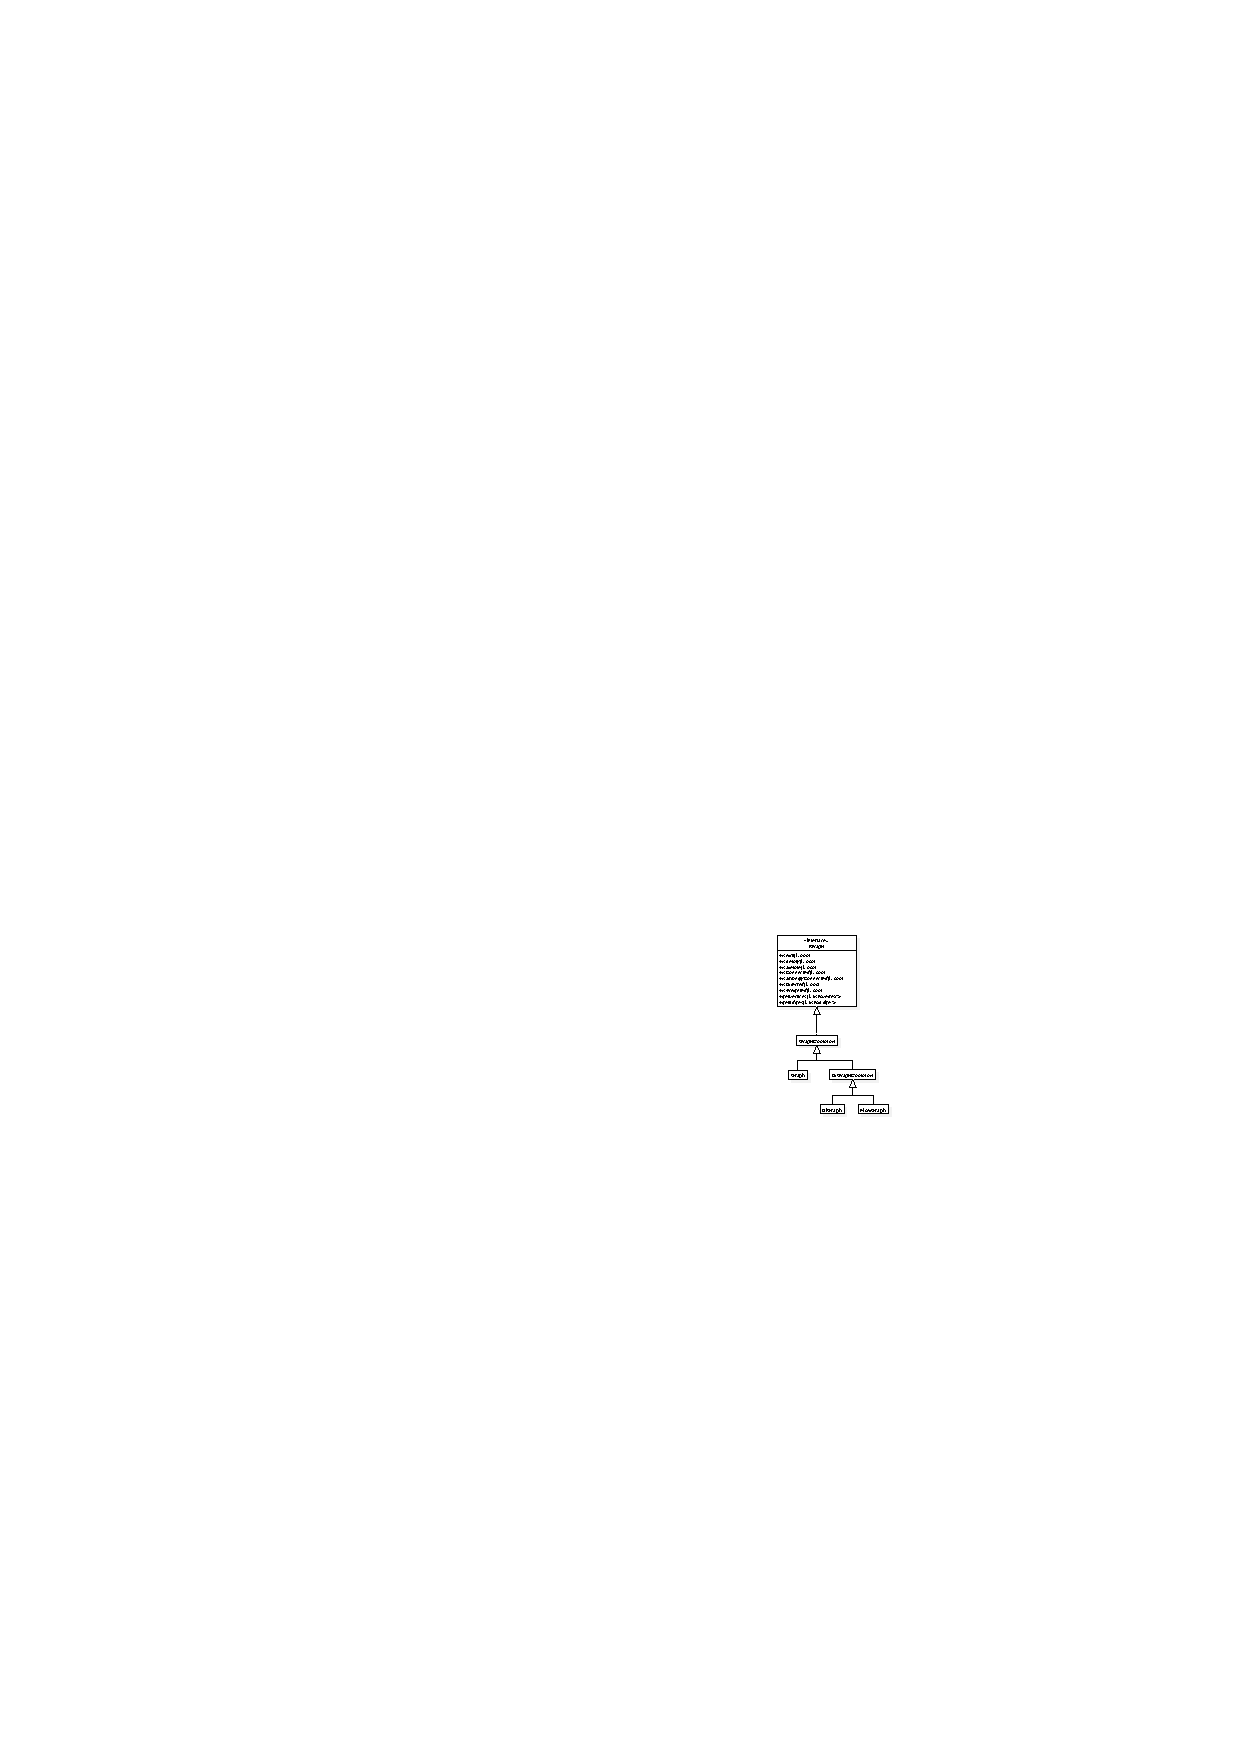
\includegraphics[scale=4.0]{Conception/graph/classGraph.pdf}
				\caption{Interface IGraph}
			\end{figure}
			Cette interface fournit les méthodes nécessaires aux utilisateurs pour manipuler n'importe quel type de graphe. La création d'un graphe se fait alors de la manière suivante :\\
			\begin{lstlisting}
						// Creation d'un graphe non-oriente vide (sans sommet)
						IGraph *graph = new Graph;
						
						// Creation d'un graphe oriente vide (sans sommet)
						IGraph *diGraph = new DiGraph;
						
						// Creation d'un graphe a flot vide (sans sommet)
						IGraph *flowGraph = new FlowGraph;
						
						// exemple de methode
						cout << graph->isDirected() << endl; // Affiche false
						cout << diGraph->isDirected() << endl; // Affiche true
						cout << flowGraph->isDirected() << endl; // Affiche true
			\end{lstlisting}
			
			\subsubsection{Structure de donnée de la classe "Graph"}
			On peut distinguer deux approches principales pour représenter et stocker un graphe :
			\begin{enumerate}
				\item à l'aide de matrices
				\item ou à l'aide de listes (ou tableaux)
			\end{enumerate}	
			L'utilisation de matrices est prépondérante dans la modélisation mathématique de nombreux problèmes et l'étude de certaines propriétés d'un graphe. Elle permet des vérifications rapides pour la présence ou non d'arcs/arêtes, mais est relativement lente lorsqu'il s'agit de les parcourir.
			
			Quant aux listes, notamment les listes d'adjacence, l'itération des arcs/arêtes est rapide mais la vérification de leur présence est lente. Les listes sont un moyen compact de représenter les matrices car elles stockent uniquement les arêtes existantes. Le gain de place mémoire est donc plus avantageux tant que le graphe n'est pas complet.\\
			
			À ce stade, le choix de l'un ou l'autre présente alors ses avantages et désavantages. Une petite étude nous a permis d'orienter notre choix : \\
			
			Une première approche simple nous permet de déterminer qu'un graphe stocké sous forme de matrice occupera $n^2$ octets, où n est le nombre de sommet. Dans ce cas, un type char ferait amplement l'affaire pour représenter chaque case, car en non-signé, on pourrait avoir jusqu'à 255 arcs/arêtes entre deux sommets.\\
			\begin{figure}[H]
				\centering
				\[
				\kbordermatrix{
					& v_1 & v_2 & v_3 & v_4 & v_5 \\
					v_1 & 0 & 2 & 4 & 1 & 1 \\
					v_2 & 0 & 0 & 0 & 0 & 1 \\
					v_3 & 1 & 0 & 0 & 0 & 1 \\
					v_4 & 0 & 3 & 0 & 0 & 1 \\
					v_5 & 1 & 1 & 0 & 3 & 0
				}
				\]
				\caption{Matrice d'adjacence de char}
			\end{figure}
			
			La seconde approche vise à réduire la taille mémoire de façon à n'avoir qu'un seul bit par case pour la présence ou non d'une arête. Cette approche économise huit fois plus de mémoire mais est inutilisable lorsqu'il y a plus de deux arêtes entre deux sommets.\\
			\begin{figure}[H]
				\centering
				\[
				\kbordermatrix{
					& v_1 & v_2 & v_3 & v_4 & v_5 \\
					v_1 & 0 & 1 & 1 & 1 & 1 \\
					v_2 & 0 & 0 & 0 & 0 & 1 \\
					v_3 & 1 & 0 & 0 & 0 & 1 \\
					v_4 & 0 & 0 & 0 & 0 & 1 \\
					v_5 & 1 & 1 & 0 & 0 & 0
				}
				\]
				\caption{Matrcide d'adjacence de bit}
			\end{figure}
			
			Ces deux premières approches ne permettent pas de stocker beaucoup d'informations concernant les Edge, c'est pourquoi nous nous tournons vers une troisième approche qui consiste à stocker des pointeurs de \lstinline[basicstyle=\ttfamily\color{blue}]|IEdge|, ou nullptr lorsque l'arc/arête n'est pas présent. Pour pouvoir stocker plusieurs Edge, chaque case contient un pointeur vers une collection d'objets \lstinline[basicstyle=\ttfamily\color{blue}]|IEdge|.
			Cette troisième approche nécessite néanmoins 32 bits par case donc une taille mémoire de 4 $*$ $n^2$ octets.\\
			\begin{figure}[H]
				\centering
				\[
				\kbordermatrix{
					& v_1 & v_2 & v_3 & v_4 & v_5 \\
					v_1 & nullptr & *edges  & nullptr & *edges  & *edges   \\
					v_2 & nullptr & nullptr & nullptr & nullptr & nullptr  \\
					v_3 & *edges  & nullptr & nullptr & nullptr & *edges   \\
					v_4 & nullptr & nullptr & nullptr & nullptr & *nullptr \\
					v_5 & *edges  & *edges  & nullptr & nullptr & nullptr
				}
				\]
				\caption{Matrice d'adjacence de collection d'Edge}
			\end{figure}				
				
			
			Cependant, après avoir suivi le cours de GRE, nous nous sommes rendus compte qu'il était rare d'obtenir des graphes complets. La majorité des cas d'utilisation requièrent des graphes de faible densité, ce qui nous amène vers une quatrième approche : stocker les graphes sous forme de liste d'adjacence.\\
			
			Mis à part les aspects liés au gain de mémoire, les listes d'adjacence facilitent la plupart des opérations présentes dans nos algorithmes.
			Trouver tous les sommets adjacents à un certain sommet est aussi simple que lire la liste et prend un temps proportionnel au nombre de voisins. Avec une matrice, toute une ligne doit être lue, ce qui prend un temps beaucoup plus long, égal au nombre de sommets présents dans le graphe entier.
			
			Cette quatrième et dernière approche est celle que nous avons choisie car elle est la plus adaptée à nos besoins. Nos graphes sont donc stockés sous forme de liste d'adjacence.
			
			\subsubsection{Détails d'implémentation de la structure}
			Dans cette partie, nous définissons comment la liste d'adjacence est implémentée. Il existe trois manières de représenter une telle liste :
			\begin{enumerate}
				\item Pour chaque sommet, lui associer un tableau des sommets adjacents. Il n'y a pas de représentation explicite des arcs/arêtes.
				\item Un tableau indexé par les numéros de sommet, où chaque case contient une simple liste chainée constituée des sommets adjacents, ou des arcs/arêtes adjacent(e)s.
				\item Une approche plus orientée objet consiste à avoir une variable d'instance pour chaque sommet, pointant vers une collection d'objets qui liste les arcs/arêtes voisin(e)s. À l'opposé, chaque arc/arête pointe vers les sommets qui la compose. 
			\end{enumerate}
			La solution (1) ne permet pas de stocker d'informations sur les arcs/arêtes. La solution (2) le permet, pour autant qu'on choisisse une liste d'Edge adjacents. Dans ce cas, on ne peut pas stocker d'information sur les sommets.\\
			
			Nous avons donc opté pour la solution (3). Un tableau de sommets, où chaque sommet possède une variable pointant vers une liste de pointeurs de \lstinline[basicstyle=\ttfamily\color{blue}]|IEdge|, et où chaque \lstinline[basicstyle=\ttfamily\color{blue}]|IEdge| possède un pointeur sur chacun des sommets qui la constitue. Nous aurions également pu stocker des pointeurs de \lstinline[basicstyle=\ttfamily\color{blue}]|T| (\lstinline[basicstyle=\ttfamily\color{blue}]|T| étant le typename du template, donc le type de l'Edge) mais pour avoir une visibilité plus globale sur les Edge, nous avons décidé de stocker des pointeurs de \lstinline[basicstyle=\ttfamily\color{blue}]|IEdge|.\\
			À noter que pour un graphe non orienté, les Edge se répéteront à double et c'est précisément ce que nous voulons car nous souhaitons préserver la logique de la liste d'adjacence pour nos algorithmes.\\
			
			Le choix de stocker les éléments par pointeur ou par copie a été longuement réfléchi. L'un comme l'autre a ses avantages et désavantages.\\ \\
			\begin{tabular}{p{0.1\textwidth}|p{0.4\textwidth}|p{0.4\textwidth}}
				 &Avantages&Désavantages\\
				\hline
				Copie& On peut passer le même Vertex déclaré une seule fois à plusieurs graphes. Même chose pour les Edge. & Prend beaucoup de place mémoire, surtout que la structure peut vite devenir grande. Un vertex ne peut pas être modifié en dehors de la structure (peut aussi être un avantage...)\\
				\hline
				Pointeur& Le sommet ou l'edge manipulé n'existe qu'une seule fois et peut être modifié depuis n'importe où (peut être dangereux) & Nécessite de gérer soi-même la désallocation de mémoire \\
			\end{tabular}
			
			L'argument de l'espace mémoire alloué a porté notre choix final sur l'utilisation de pointeurs pour stocker les éléments.			
		
			Voici un exemple de liste d'adjacence. *e$\{chiffre\}$ est un pointeur sur l'Edge $\{chiffre\}$. Les chiffres en marge à gauche sont les index des sommets.
			\begin{figure}[H]
				\centering
				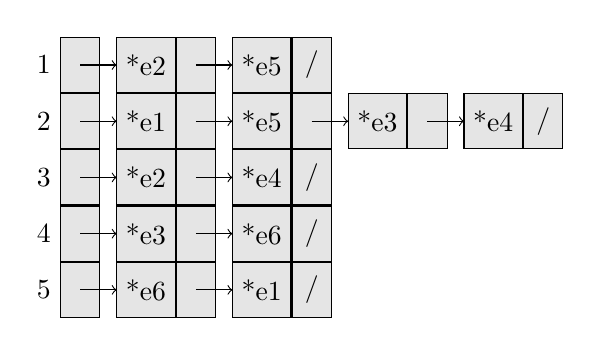
\begin{tikzpicture}
				\matrix (M) [matrix of nodes,
				column sep=0pt,
				row sep=0pt,
				nodes={draw,fill=gray!20,minimum width=.5cm,outer sep=0pt,minimum
					height=.7cm,anchor=center},
				column 1/.style={minimum height=.8cm}]{
					\mbox{} &[2mm] *e2 & \mbox{} &[2mm] *e5 & $/$     &[2mm]&         &[2mm]& \\
					\mbox{} &[2mm] *e1 & \mbox{} &[2mm] *e5 & \mbox{} & *e3 & \mbox{} & *e4 & $/$  \\
					\mbox{} &[2mm] *e2 & \mbox{} &[2mm] *e4 & $/$     &[2mm]&         &[2mm]& \\
					\mbox{} &[2mm] *e3 & \mbox{} &[2mm] *e6 & $/$     &[2mm]&         &[2mm]& \\
					\mbox{} &[2mm] *e6 & \mbox{} &[2mm] *e1 & $/$     &     &         &     & \\
				};
				\foreach \i in {1,2,3,4,5}{
					\path (M-\i-1) [late options={label=left:\i}];
					\draw[->] (M-\i-1.center)--(M-\i-2.west);
					\draw[->] (M-\i-3.center)--(M-\i-4.west);
				}
				\draw[->] (M-2-5.center)--(M-2-6.west);
				\draw[->] (M-2-7.center)--(M-2-8.west);
				\end{tikzpicture}
				\caption{Liste d'adjacence}
			\end{figure}
			Dans cet exemple:
			\begin{itemize}
				\item le sommet 1 possède deux Edge adjacents e2 et e5.
				\item le sommet 2 possède quatre Edge adjacents e1, e5, e3, e4.
				\item le sommet 3 possède deux Edge adjacents e2 et e4.
				\item etc.
			\end{itemize}
			
			Et voici à quoi ressemble le code de cette structure. À noter que nous avons besoin de garder un tableau des sommets.
			\begin{lstlisting}
						template <typename T>
						class GraphCommon : public IGraph {
							private:
								vector<Vertex*> _vertices;
								vector<list<IEdge*>> _adjacentList;
							public:
								template <typename Func>
								void forEachAdjacentEdge(Vertex v, Func f) {
									for (Edge* e : adjacentList[v->getId()]) 
										f(e); // operation sur les edges adjacents au sommet v
								}
						};
			\end{lstlisting}
			
			\subsubsection{Création de graphes}
			La création de graphe peut maintenant s'effectuer de la manière suivante :
			\begin{lstlisting}
						// Creer un graphe non oriente
						public static void main() {
							// creer quelques sommets et edges
							Vertex *v1 = new Vertex;
							Vertex *v2 = new Vertex;
							Vertex *v3 = new Vertex;
							IEdge *e1 = new Edge(v1, v2);
							IEdge *e2 = new Edge(v1, v3);
							
							vector<Vertex*> vertices = {v1, v2, v3};
							vector<IEdge*> edges = {e1, e2};
							
							// Creation d'un graphe non oriente
							IGraph *myGraph = new Graph(vertices, edges);
							
							// Utilisation d'une methode de l'interface
							if (myGraph->isSimple())
								cout << "myGraph est simple" << endl;
						}
			\end{lstlisting}
			\begin{lstlisting}
						// Creer un graphe oriente
						public static void main() {
							// creer quelques sommets et edges
							Vertex *v1 = new Vertex;
							Vertex *v2 = new Vertex;
							Vertex *v3 = new Vertex;
							IEdge *e1 = new DiEdge(v1, v2);
							IEdge *e2 = new DiEdge(v1, v3);
							
							vector<Vertex*> vertices = {v1, v2, v3};
							vector<IEdge*> edges = {e1, e2};
							
							// Creation d'un graphe oriente
							IGraph *myGraph = new DiGraph(vertices, edges);
							
							// Utilisation d'une methode de l'interface
							if (myGraph->isSimple())
								cout << "myGraph est simple" << endl;
						}
			\end{lstlisting}
			\begin{lstlisting}
						// Creer un graphe oriente a flot
						public static void main() {
							// creer quelques sommets et edges
							Vertex *v1 = new Vertex;
							Vertex *v2 = new Vertex;
							Vertex *v3 = new Vertex;
							IEdge *e1 = new FlowEdge(v1, v2);
							IEdge *e2 = new FlowEdge(v1, v3);
							
							vector<Vertex*> vertices = {v1, v2, v3};
							vector<IEdge*> edges = {e1, e2};
							
							// Creation d'un graphe oriente a flot
							IGraph *myGraph = new FlowGraph(vertices, edges);
							
							// Utilisation d'une methode de l'interface
							if (myGraph->isSimple())
								cout << "myGraph est simple" << endl;
						}
			\end{lstlisting}
			
		\subsection{Algorithmes}
			\subsubsection{Pattern Visitor}
			Le patron de conception Visiteur permet d'appliquer efficacement un algorithme à un graphe. L'utilisation est la suivante :
			\begin{itemize}
				\item L'algorithme est le visiteur
				\item Le graphe représente la structure de donnée à visiter
			\end{itemize}
			L'interface Visitor peut visiter un \lstinline[basicstyle=\ttfamily\color{blue}]|Graph|, un \lstinline[basicstyle=\ttfamily\color{blue}]|DiGraph|, ou un \lstinline[basicstyle=\ttfamily\color{blue}]|FlowGraph| et ce en spécifiant un sommet source "from" et un sommet destination "to". Tous nos algorithmes n'utiliseront pas "from" et "to", c'est pourquoi ils ont une valeur par défaut à nullptr.
			
			Le résultat de nos algorithmes retournent parfois un graphe, parfois un tableau. Deux méthodes supplémentaires \lstinline[basicstyle=\ttfamily\color{blue}]|IGraph *G();| et \lstinline[basicstyle=\ttfamily\color{blue}]|vector<double> table();| ont donc été ajoutées.
			
			Du côté de la structure, une méthode \lstinline[basicstyle=\ttfamily\color{blue}]|accept(Visitor *v, Vertex *from, Vertex *to)| permet de spécifier au visiteur quel type de graphe manipuler au travers de la liaison dynamique.
			
			Finalement, une classe statique \lstinline[basicstyle=\ttfamily\color{blue}]|GraphAlgorithm| liste tous les algorithmes implémentés (voir dans la section "liste des algorithmes implémentés").
			
			\begin{figure}[H]
				\centering
				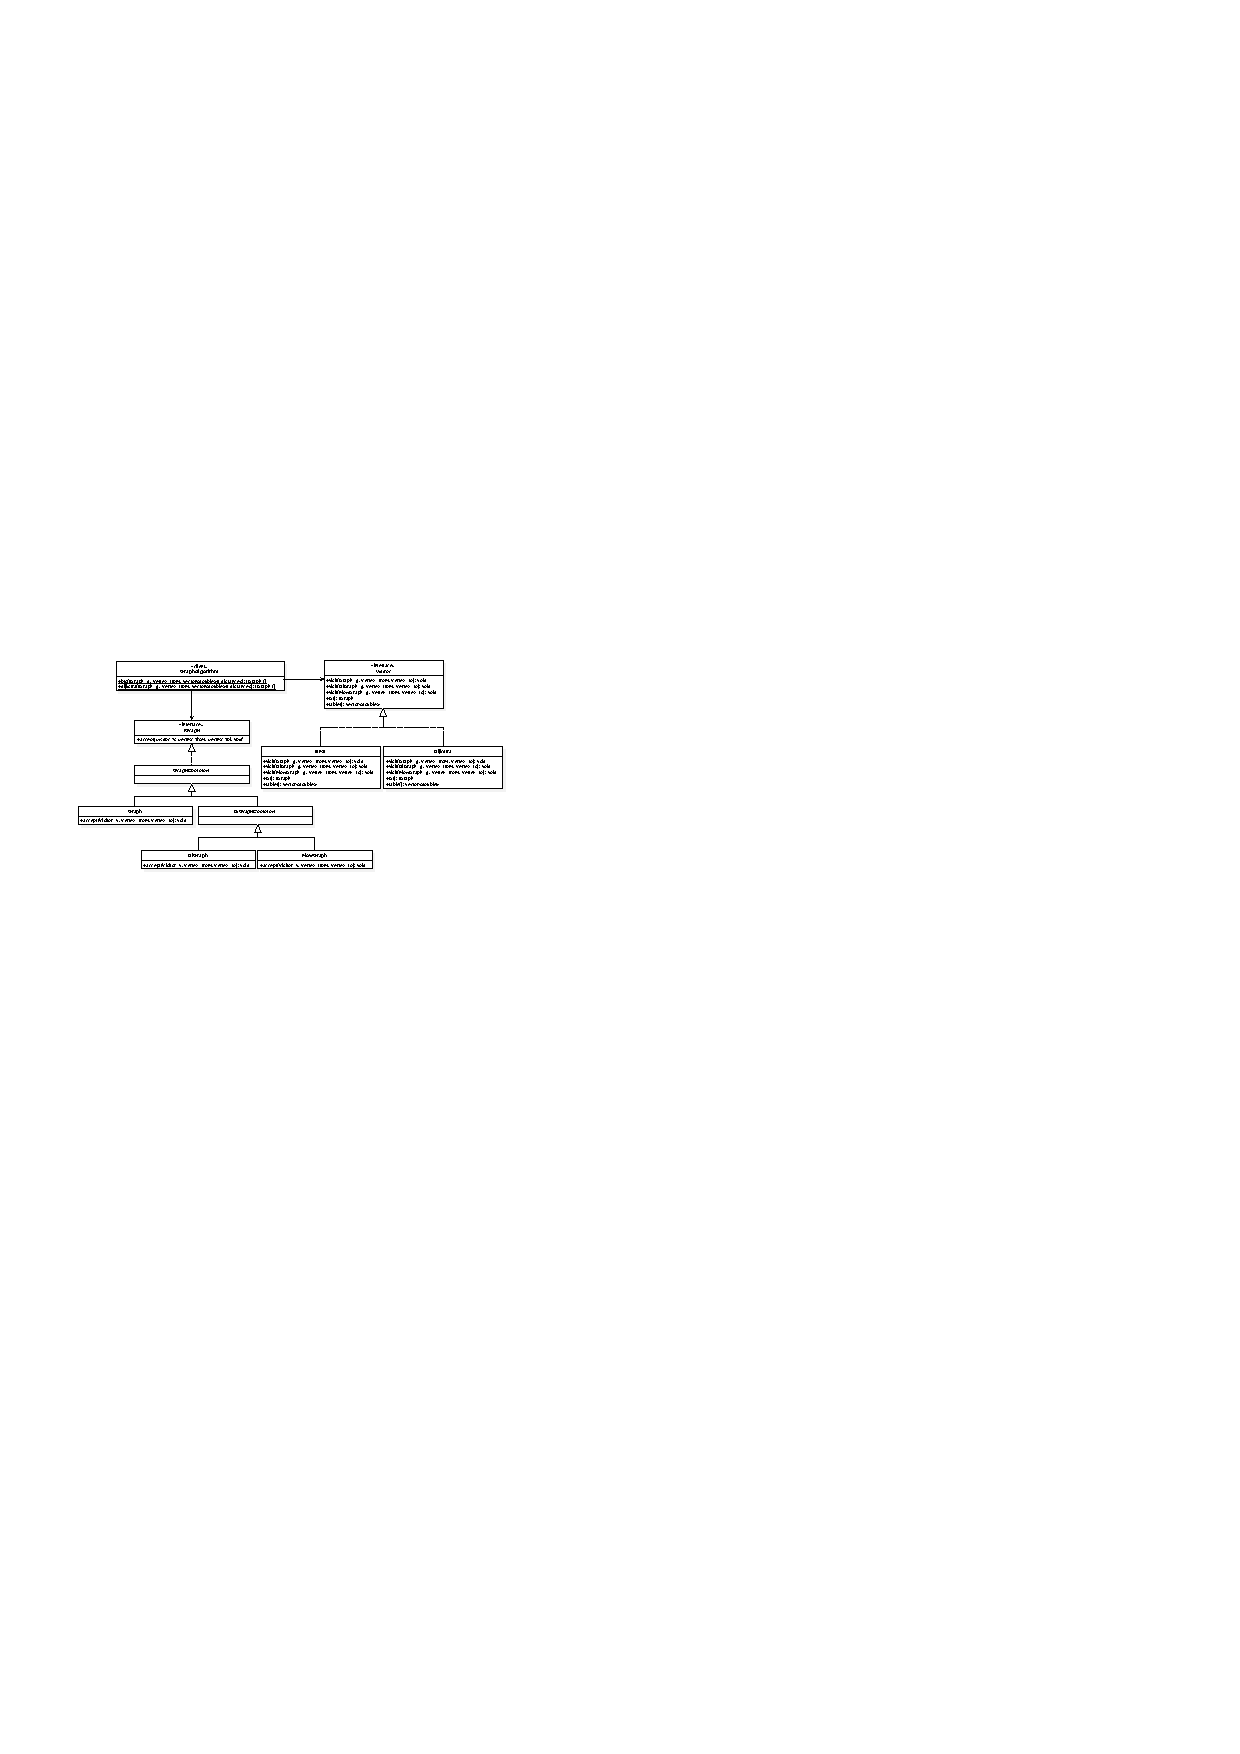
\includegraphics[scale=2.4]{Conception/graph/visitor.pdf}
				\caption{Pattern Visitor pour l'application des algorithmes aux graphes}
			\end{figure}
			
			Les algorithmes ne sont pas les mêmes pour tous les types de graphe : un parcours en largeur sera quelque peu différent entre un graphe orienté et non-orienté. Le pattern Visiteur est précisément fait pour répondre à ce genre de problème. De plus, l'avantage du pattern est qu'il est facilement extensible : un nouvel algorithme s'ajoute tout bonnement en tant que visiteur. Par contre, la structure de donnée doit être complète et tout changement de cette dernière demandera, selon le changement, une adaptation chez tous les visiteurs.\\
			
			\begin{lstlisting}
						// Code d'un objet visite
						class Graph {
							private:
								//...
							public:
								void accept(Visitor *v, Vertex *from, Vertex *to) {
									v->visitGraph(this, from, to);
								}
						};
			\end{lstlisting}
			\begin{lstlisting}
						// Implementation d'un visiteur
						class BFS : public Visitor {
							private:
								vector<double> _distances;
								IGraph *_G;
								
							public:
								BFS() : _distances(0), _G(nullptr) {}
								void visit(Graph *g, Vertex *from, Vertex *to) {
									// Implementation du BFS pour un graphe non-oriente...
								}
								void visit(DiGraph *g, Vertex *from, Vertex *to) {
									// Implementation du BFS pour un graphe oriente...
								}
								void visit(FlowGraph *g, Vertex *from, Vertex *to) {
									// Implementation du BFS pour un graphe a flot...
								}
								IGraph* G() const {
									return _G;
								}
								vector<double> table() {
									return _distances;
								}
						};
			\end{lstlisting}
			\begin{lstlisting}
						// Implementation de deux algorithmes dans GraphAlgorithm
						#include "BFS.h"
						#include "Dijkstra.h"
						
						class GraphAlgorithm {							
							public:
								IGraph *bfs(IGraph *g, Vertex *from, vector<double>& distances) {
									Visitor *v = new BFS;
									g->accept(v, from);
									distances = v->table();
									return v->G();
								}
								
								IGraph *dijkstra(IGraph *g, Vertex *from, vector<double>& distances) {
									Visitor *v = new DijkstraSP;
									g->accept(v, from);
									distances = v->table();
									return v->G();
								}
						};
			\end{lstlisting}
			
			Nous avons choisi ce pattern car il permet de bien séparer la structure de donnée des algorithmes et il nous permet de collaborer efficacement au sein de l'équipe.
			
			\subsubsection{Liste des algorithmes implémentés}
			Dans le tableau ci-dessous figurent les algorithmes traités par l'application. Pour la colonne \textit{Complexité}, $V$ représente le nombre de sommet (Vertex), et $E$ le nombre d'arcs/arêtes (Edge) d'un graphe.
			\begin{figure}[H]
				\centering
				\begin{tabular}{L{2cm}L{3cm}L{8cm}l}
					\textbf{Nom} & \textbf{Valeur de retour} & \textbf{Description} & \textbf{Complexité}\\
					\hline
					BFS & IGraph & Breadth First Search : effectue une exploration en largeur d'un graphe depuis un sommet source et retourne l'arborescence du parcours. & $O(V+E)$\\
					\hline
					DFS & IGraph & Depth First Search : effectue une exploration en profondeur d'un graphe depuis un sommet source et retourne l'arborescence du parcours. & $O(V+E)$\\
					\hline
					Composante connexe & vector<double> & Calcule les composantes connexes d'un graphe et retourne un tableau dont l'index représente le sommet et la valeur la composante à laquelle appartient le sommet. & $O(V+E)$\\
					\hline
					Composante fortement connexe & vector<double> &Calcule les composantes fortement connexes d'un graphe orienté et retourne un tableau dont l'index représente le sommet et la valeur de la composante à laquelle appartient le sommet. & $O(V+E)$\\
					\hline
					Kruskal & IGraph et vector<double> en paramètre  &Implémenté avec UnionFind, recherche de l'arbre recouvrant de poids minimum. & $O(E * log(V))$\\
					\hline
					Bellman-Ford & IGraph et vector<double> en paramètre &Recherche les plus courts chemins depuis un sommet source vers tous les autres sommets. Le graphe doit être orienté et pondéré. & $O(E*V)$\\
					\hline
					Dijkstra & IGraph et vector<double> en paramètre & Implémenté à l'aide d'une queue de priorité, recherche d'un plus court chemin depuis un sommet source vers tous les autres sommets. Le graphe doit être orienté et pondéré positivement (ou nul). & $O(E * log(V))$\\
                                       \hline
					Detection des cycles & IGraph & Détermine si un graphe contient un cycle ou un circuit pour les graphes orientés et retourne le cycle trouvé. & $O(E+V))$\\
                                      \hline
				      Tri Topologique & vector<double> & recherche l'ordre par lequel il faut parcourir le graphe topologiquement. Le graphe doit être orienté ou à flow. & $O(E+V))$\\

				\end{tabular}
			\end{figure}
			
			\subsubsection{Utilisation}
			L'utilisation se fait de la manière suivante
			\begin{enumerate}
				\item Créer un graphe (avec des sommets et des edges) 
				\item Appeler l'algorithme voulu
				\item Récupérer le graphe résultant de l'algorithme (si l'algorithme retourne un graphe), sinon récupérer le tableau de double (et éventuellement le tableau de doubles passé préalablement en paramètre)
			\end{enumerate}
			
			\begin{lstlisting}
						// Exemple d'utilisation
						#include "Graph.h"
						#include "GraphAlgorithm.h"
						
						int main {				
							// Creation d'un graphe non oriente
							Vertex *v1 = new Vertex;
							Vertex *v2 = new vertex;
							Vertex *v3 = new vertex;
							
							IEdge *e1 = new Edge(v1, v2);
							
							IGraph *g = new Graph;
							
							g->addVertex(v1);
							g->addVertex(v2);
							g->addVertex(v3);
							g->addEdge(e1);
							
							// Application d'un BFS depuis v1
							vector<double> distances;
							IGraph *bfs = GraphAlgorithm::bfs(g, v1, distances);
							
							// Resultat
							cout << *bfs << endl;		// Affiche v1--v2
							for (double d : distances)	
								cout << d << " ";		// Affiche 0 1 -1
							cout << endl;
							
							return EXIT_SUCCESS;
						};
			\end{lstlisting}
			


	\section{Conclusion}
		% Conclusion critique sur l'application fournie et le travail de groupe
		% Indications précises de ce qui ne fonctionne pas correctement
		% Propositions d'améliorations pour des développements futurs
	
		\subsection{Application fournie}			
			Vis à vis du cahier des charges initial (disponible en annexe), l'application répond à toutes les fonctionnalités prévues hormis l'implémentation de certains algorithmes, dont voici la liste:
			\begin{itemize}
				\item Arborescence recouvrante de poids min
				\item Arborescence recouvrante de section min/max
				\item Flot de capacité fixée (ou min)
				\item Flot de capacité fixée (ou min) de poids min
			\end{itemize}
			Les fonctionnalités optionnelles et futures n'ont pas pu être intégrées par manque de temps, cependant leur ajout est tout à fait réalisable car la conception générale de l'application a été prévue pour être ouverte aux extensions. Notons encore que l'interface graphique n'est pas tout à fait la même que la maquette présente dans le cahier des charges, néanmoins les fonctionnalités sont les mêmes.\\
			
			Concernant la stabilité du programme, la majorité des bugs/crashs découverts pendant le projet a été corrigée. Cependant certains cas posent toujours problème:
			\begin{enumerate}
				\item Un graphe ne possédant pas tous les sommets dans l'ordre (ex: \texttt{g=dfs(\{\#2\}, 1);}) pose problème à certaines fonctionnalités (ex: \texttt{draw(g);}, \texttt{egli::deserialize(...);})
				\item Fuites mémoires détectées au niveau de la couche \textit{graphes et algorithmes}
				\item La fenêtre d'aide ne se ferme pas lorsque que l'on quitte la fenêtre principale (avec la croix en haut à droite)
				\item La grammaire du langage ne permet pas de tout faire (ex: \texttt{v=(0); g=\{v\};}, \texttt{v=(0::-1);}, \texttt{draw(dfs(g, 0)[0]);})
			\end{enumerate}
			Les cas (1) et (2) sont des priorités absolues pour la suite du développement, mais nous les avons malheureusement découverts trop tard pour pouvoir les corriger en l'état. Par chance, les causes des problèmes sont connues, ce qui permettra de les corriger rapidement. De plus, nous avons découvert l'existence du logiciel DrMemory \cite{drmemory} qui nous offre la possibilité de cibler les fuites mémoires très précisément.\\
			
			Un petit mot sur le langage développé spécifiquement pour l'application. Celui-ci demande un petit temps d'apprentissage, mais la prise en main est assez rapide. L'aide intégrée et ses pages bien expliquées (facilement extensible), sa fonction de recherche par mots-clés, ainsi que l'auto-complétion des fonctions et variables prend l'utilisateur par la main et rend l'utilisation de l'application agréable.\\  
			
			Au final, nous sommes satisfaits du résultat final bien qu'il reste encore d'importants bugs à corriger. Le projet offre de nombreuses possibilités d'amélioration, tant au niveau de l'interface graphique que du reste, et nous sommes très contents de cela. Voici une liste non-exhaustive des améliorations possibles auxquelles nous avons pensées:
			\begin{itemize}
				\item Meilleure visualisation des graphes
				\item Affichage des variables créées dans une zone de l'interface graphique
				\item Coloration syntaxique
				\item Fonctionnalités optionnelles et futures du cahier des charges
				\item ... et plein d'autres
			\end{itemize}
		
		\subsection{Planification}
			% Les figures ne prennent pas en compte les tests et la doc, uniquement la conception et l'impl.
			
			La planification initiale du projet (disponible en annexe) a fait ressortir plusieurs problèmes. Premièrement, les temps d'analyse et de conception ont été très largement sous-estimés, ce qui a engendré un gros décalage des tâches:
			\begin{figure}[H]
				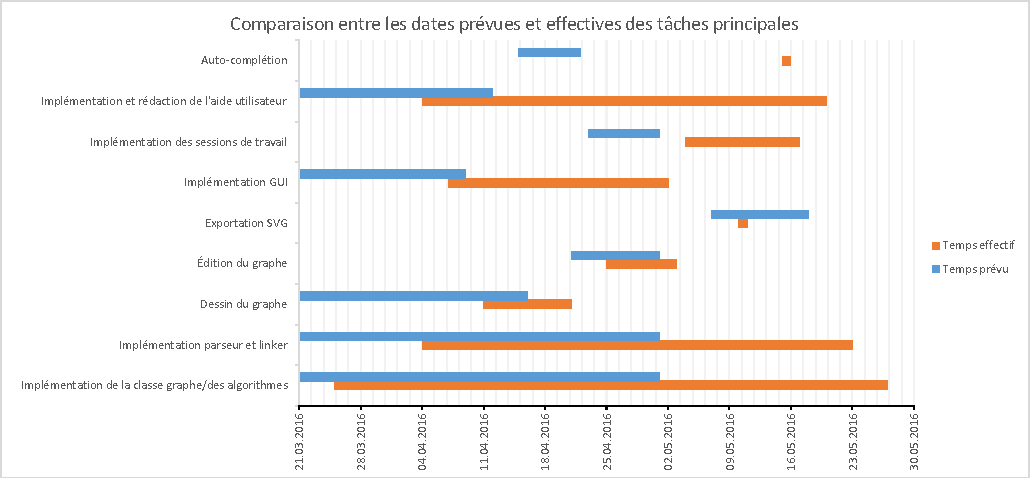
\includegraphics[width=\textwidth]{Planification/comparaisondates.pdf}
				\caption{Comparaison entre les dates prévues et effectives des tâches principales}
				\label{fig:comparaisondates}
			\end{figure}
			On peut expliquer cela par deux choses: certains problèmes étaient plus complexes que prévus, et l'apprentissage de Qt était beaucoup plus long. En effet, Qt est très puissant et offre de multiples manières d'aborder un problème, en contre-partie cela induit des pertes de temps lorsque l'on part dans la mauvaise direction. Cependant une fois que Qt est pris en main, les gains lors de l'implémentation sont conséquents.\\ 
			
			Deuxièmement, la planification initiale était une suite de tâches à faire complètement avant de passer à la suivante. Dans les faits, les tâches (pour une même personne) ont été réalisées en parallèle, cela a impliqué une dissonance entre les temps prévus et les temps effectifs.\\
			
			Troisièmement, la partie sur les graphes et les algorithmes a été la plus largement sous-estimée, le graphique suivant le montre assez clairement:
			\begin{figure}[H]
				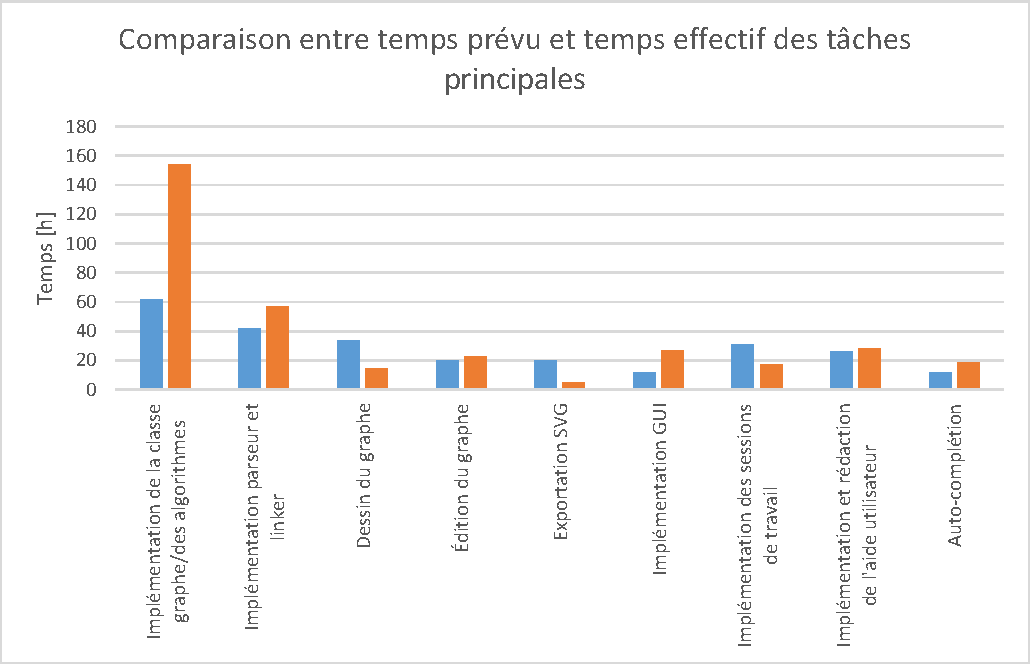
\includegraphics[width=\textwidth]{Planification/comparaisonheures.pdf}
				\caption{Comparaison entre le temps prévu et temps effectif des tâches
					principales}
				\label{fig:comparaisonheures}
			\end{figure}
			
			Pour finir, les différentes tâches, bien que mal planifiées, ont été bien cernées dès le début du projet. Cela a permis une séparation du travail correcte et indépendante, ainsi qu'une application finale utilisable. Nous sommes cependant convaincus qu'utiliser un modèle de développement itératif (et non pas en cascade) aurait apporté un plus au projet. En effet, cela nous aurait obligé à mettre les différentes couches en commun plus souvent, et ainsi détecter les problèmes avant la fin du projet. 
		
		\subsection{Travail de groupe}
			Le principal problème, comme mentionné dans la section précédente, a été le fait que nous n'avons pas fixé suffisamment de délais intermédiaires et que la mise en commun n'a été faite qu'à la fin du projet. Cela a posé des problèmes que nous n'avons malheureusement pas pu résoudre dans les temps.\\
			
			Le second problème a été un laxisme en début de semestre, nous avons donc dû fournir un gros effort lors des dernières semaines. Lors de ces "rushs", où nous avons travaillé tous ensemble dans la même pièce, il a été intéressant de constater la grande efficacité avec laquelle nous avons travaillé. En effet les problèmes se résolvent beaucoup plus vite et l'ambiance offre un cadre de travail beaucoup plus motivant et encourageant. Il nous semble donc important à l'avenir de planifier ce type de séance plus souvent tout au long d'un projet, pour une meilleure productivité.\\
			
			Pour conclure, ce projet a été une expérience enrichissante, autant du point de vue technique et de la planification, que du travail en grand groupe. La collaboration au sein de l'équipe a été très bonne durant toute la durée du semestre, et cela même malgré la grande charge de travail avec les autres cours. Nous sommes donc au final heureux d'avoir pu participer à l'élaboration de A à Z d'un projet complet et complexe, nous profitons de cette conclusion pour nous remercier les uns les autres pour le travail accompli.
			
			\newpage
	% Tables des figures
	\listoffigures
			
	% References
	\begin{thebibliography}{9}
		\bibitem{qtStyle}
		Qt wiki, Qt coding style,\\ \url{https://wiki.qt.io/Qt_Coding_Style}
		
		\bibitem{vutbr.cz} 
		Faculty of Technology, Brno University of Technology, République tchèque,\\ \url{http://www.fit.vutbr.cz/study/courses/APR/public/ebnf.html}
		
		\bibitem{plantuml}
		PlantUML, Open-source tool that uses simple textual descriptions to draw UML diagrams,\\ \url{http://plantuml.com/}\\ \url{http://www.planttext.com/planttext}
		
		\bibitem{Graph data wikipedia.org}
		Graphs data structures,\\ \url{https://en.wikipedia.org/wiki/Adjacency_matrix#Data_structures}
		
		\bibitem{boost.spirit}
		Boost.Spirit (v2.5.2), is an object-oriented, recursive-descent parser and output generation library for C++,\\ \url{http://www.boost.org/doc/libs/1_60_0/libs/spirit/doc/html/index.html}
		
		\bibitem{tries}
		Robert Sedgewick, Kevin Wayne.\\
		\emph{Algorithms, fourth edition}\\
		\url{http://algs4.cs.princeton.edu/lectures/52Tries.pdf}
		
		\bibitem{sedgewick}
		Robert Sedgewick.\\
		\emph{Course on ternary search tries}
		\url{https://www.youtube.com/watch?v=CIGyewO7868}
		
		\bibitem{drmemory}
		DrMemory,\\
		\url{http://drmemory.org/}
	\end{thebibliography}
			
	\newpage
	\section{Annexes EGLI}
	\label{sec:annexes-egli}
	
		\subsection{Grammaire EBNF} 
		L'analyse étant finie (section~\ref{subsubsec:analyse-des-types-et-des-operations}), on peut à présent développer les règles de production EBNF du langage. On part des règles de haut niveau pour descendre dans la hiérarchie (inspiration: \cite{vutbr.cz}).\\
		
		\textbf{Point de départ (entrée utilisateur)}
		\begin{grammar}
			<start> ::= <statement> \{ <statement> \}
		\end{grammar}
		
		\textbf{Déclarations (statements)}
		\begin{grammar}
			<statement> ::= ( <function-call> | <declaration> | <assignation> ) \lit{;}
			
			<function-call> ::= <identifier> <parameter-list>
			
			<declaration> ::= <type> <identifier> \lit{=} <parameter>
			
			<assignation> ::= <variable> \lit{=} <parameter>
			
			<parameter-list> ::= \lit{(} <parameter> \{ \lit{,} <parameter> \} \lit{)}
			
			<parameter> ::= <constant> | <indexed-array> | <function-call>
		\end{grammar}
		
		\textbf{Expressions et opérations}
		\begin{grammar}
			<indexed-array> ::= <variable> \lit{[} <digit-sequence> \lit{]}
		\end{grammar}
		
		\textbf{Types de variable et d'enregistrement}
		\begin{grammar}
			<type> ::= <simple-type> | <complex-type>
			
			<simple-type> ::= \lit{Boolean} | \lit{Number} | \lit{Integer} | \lit{Float} | \lit{String}
			
			<complex-type> ::= \lit{Array} | \lit{Graph} | \lit{Vertex} | \lit{Edge}
			
			<array-record> ::= \lit{[} <constant> \{ \lit{,} <constant> \} \lit{]}
			
			<constant> ::= <simple-constant> | <complex-constant>
			
			<complex-constant> ::= <array-record> | <graph-record> | <edge-record> | <vertex-record>
			
			<graph-record> ::= \lit{\{} <graph-info> \{ \lit{,} <graph-info> \} \lit{\}}
			\alt \lit{\{} \lit{\#} <digit-sequence> \{ \lit{,} <graph-info> \} \lit{\}}
			
			<edge-record> ::= \lit{(} <edge-info> \lit{)}
			
			<vertex-record> ::= \lit{(} <vertex-info> \lit{)}
			
			<graph-info> ::= <vertex-info> | <edge-info>
			
			<edge-info> ::= <connection> 
			\alt <connection> \lit{:} <number>
			\alt <connection> \lit{:} [ <number> ] \lit{:} <string>
			\alt <connection> \lit{:} [ <number> ] \lit{:} [ <string> ] \lit{:} <number>
			\alt <connection> \lit{:} [ <number> ] \lit{:} [ <string> ] \lit{:} [ <number> ] \lit{:} <number>
			
			<vertex-info> ::= <id> 
			\alt <id> \lit{:} <string>
			\alt <id> \lit{:} [ <string> ] \lit{:} <number>
			\alt <id> \lit{:} [ <string> ] \lit{:} [ <number> ] \lit{:} <number>
			\alt <id> \lit{:} [ <string> ] \lit{:} [ <number> ] \lit{:} [ <number> ] \lit{:} <number>
			
			<connection> ::= <id> ( \lit{\textendash\textemdash} | \lit{\textemdash\textgreater} | \lit{\textless\textemdash} ) <id>
			
			<id> ::= <digit-sequence>
		\end{grammar}
		
		\textbf{Identifiants et définitions de bas niveau}
		\begin{grammar}
			<simple-constant> ::= <sign> <variable> | <number> | <boolean> | <string>
			
			<variable> ::= <identifier>
			
			<identifier> ::= <letter> \{ <letter> | <digit> | \lit{\_} \}
			
			<string> ::= \lit{"\""} \{ <letter> | \lit{ } \} \lit{"\""}
			
			<letter> ::= ? all lower and upper case letters ? 
			
			<boolean> ::= \lit{True} | \lit{False}
			
			<number> ::= <integer-number> | <real-number>
			
			<real-number> ::= [ <sign> ] <digit-sequence> \lit{.} <digit-sequence>
			
			<integer-number> ::= [ <sign> ] <digit-sequence>
			
			<digit-sequence> ::= <digit> \{ <digit> \}
			
			<sign> ::= \lit{+} | \lit{-} 
			
			<digit> ::= ? all digits from 0 to 9 ? 
		\end{grammar}
		
		\subsubsection{Modifications}
		\textbf{24.04.2016}\\
		Après réflexion, il est apparu que les opérations d'assignation et de déclaration de variables pouvaient être mises ensemble. Concrètement dans une déclaration il n'est pas nécessaire de définir le type de la variable car celui-ci peut être déduit de l'opérande de droite. Et comme les tableaux sont des collections hétérogènes, il semble évident que les variables doivent elles aussi être à typage dynamique. Par conséquent la grammaire est modifiée ainsi:
		\begin{itemize}
			\item Suppression des règles \textit{<declaration>}, \textit{<type>}, \textit{<simple-type>} et \textit{<complex-type>}
			\item La règle \textit{<assignation>} vaut désormais: \textit{( <variable> | <identifier> ) '=' <parameter>}
			\item La règle \textit{<statement>} vaut désormais: \textit{( <function-call> | <assignation> ) ';'}
		\end{itemize} 
		
		\textbf{12.05.2016}\\
		Pendant l'implémentation du parseur, des oublis dans la grammaire ont été constatés, voici les règles manquantes:
		\begin{itemize}
			\item Nouvelle règle: \textit{<graph-add> ::= <identifier> '+=' <parameter>}
			\item Nouvelle règle: \textit{<graph-sub> ::= <identifier> '-=' <parameter>}
			\item La règle \textit{<connection>} vaut désormais: \textit{<id> ( '\textendash-' | '->' | '<-' ) <id> [ '[' <digit-sequence> ']' ]}
			\item La règle \textit{<statement>} vaut désormais: \textit{( <function-call> | <assignation> | <graph-add> | <graph-sub> ) ';'}
		\end{itemize}
		De plus, en l'état, l'implémentation ne permet pas d'écrire par exemple \texttt{v = (0:label);} ou \texttt{v = (0::-2);}, cela à cause des règles qui n'utilisent pas assez la règle \textit{<parameter>}. Cela peut être une amélioration future.
		
		\subsection{Flux des données}
		\begin{figure}[H]
			\centering
			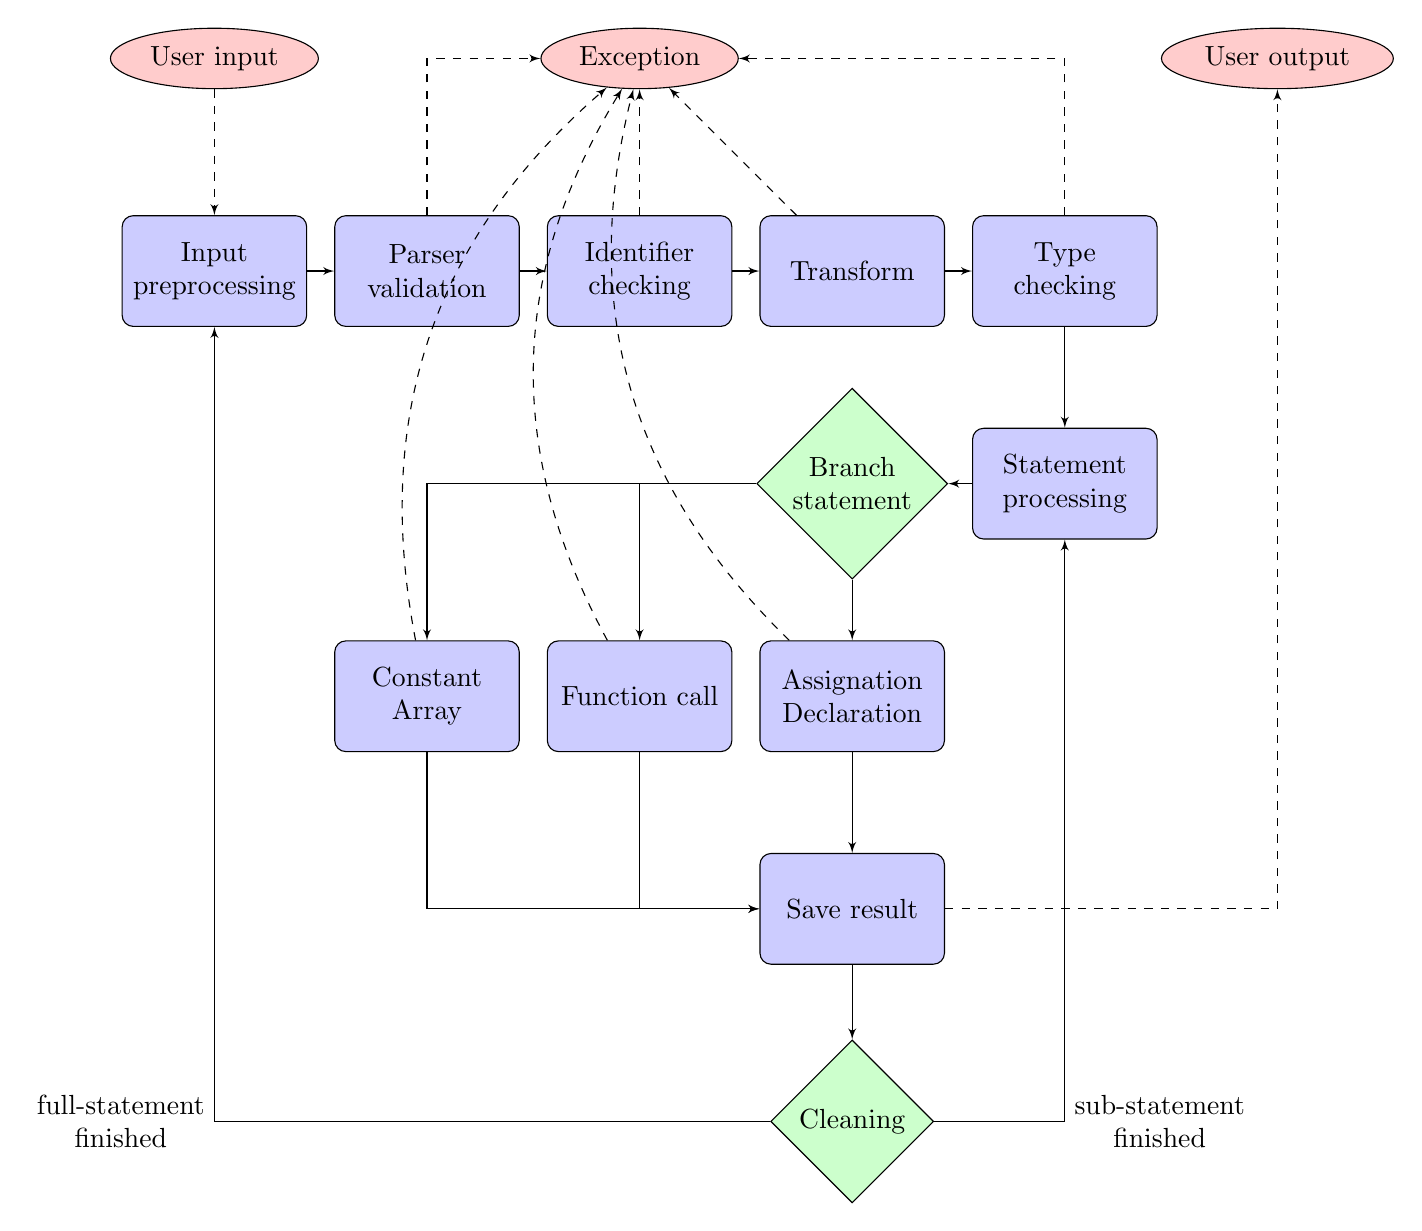
\begin{tikzpicture}[decision/.style = {diamond, draw, fill=green!20, text width=5em, text badly centered, inner sep=0pt}, block/.style = {rectangle, draw, fill=blue!20, text width=6em, text centered, rounded corners, minimum height=4em}, line/.style = {draw, -latex'}, cloud/.style = {draw, ellipse,fill=red!20, minimum height=2em}, node distance = 2.7cm,auto]
			\node[cloud] (input) {User input};
			\node[block,below of=input] (preprocessor) {Input preprocessing};
			\node[block,right of=preprocessor] (parser) {Parser validation};
			\node[block,right of=parser] (identifier) {Identifier checking};
			\node[cloud,above of=identifier] (exception) {Exception};
			\node[block,right of=identifier] (transformation) {Transform};
			\node[block,right of=transformation] (type) {Type checking};
			\node[block,below of=type] (parameter) {Statement processing};
			\node[decision,left of=parameter] (execute) {Branch statement};
			\node[block,below of=execute] (assign) {Assignation Declaration};
			\node[block,left of=assign] (function) {Function call};
			\node[block,left of=function] (constant) {Constant Array};
			\node[block,below of=assign] (result) {Save result};
			\node[decision,below of=result] (clean) {Cleaning};
			\node[cloud,right of=type,above of=type] (output) {User output};
			
			\path[line,dashed] (input) -- (preprocessor);
			\path[line,dashed] (parser) |- (exception);
			\path[line,dashed] (identifier) -- (exception);
			\path[line,dashed] (type) |- (exception);
			\path[line,dashed] (transformation) -- (exception);
			\path[line,dashed] (function) edge[bend left] (exception);
			\path[line,dashed] (constant) edge[bend left] (exception);
			\path[line,dashed] (assign) edge[bend left] (exception);
			\path[line] (preprocessor) -- (parser);
			\path[line] (parser) -- (identifier);
			\path[line] (identifier) -- (transformation);
			\path[line] (transformation) -- (type);
			\path[line] (type) -- (parameter);
			\path[line] (parameter) -- (execute);
			\path[line] (execute) -| (function);
			\path[line] (execute) -- (assign);
			\path[line] (execute) -| (constant);
			\path[line] (function) |- (result);
			\path[line] (assign) -- (result);
			\path[line] (constant) |- (result);
			\path[line] (result) -- (clean);
			\path[line] (clean) -| node[align=center,right] {sub-statement\\finished} (parameter);
			\path[line] (clean) -| node[align=center] {full-statement\\finished} (preprocessor);
			\path[line,dashed] (result) -| (output);
			\end{tikzpicture}
			\caption{Flux des données dans l'interpréteur}
		\end{figure}
		
		Détaillons chacune de ces étapes:
		\begin{enumerate}
			\item \textbf{Input preprocessing} - On récupère les entrées utilisateur dans un tampon.
			\begin{enumerate}
				\item \textbf{Trim} - On enlève tous les espaces inutiles, c'est-à-dire tous les espaces sauf ceux dans les constantes littérales de type \textit{String}, et celui qui sépare le type de l'identifiant dans les déclarations.
				\item \textbf{Statement per statement} - On envoie au parseur une commande à la fois (les traitements sont séparés par des ';').
			\end{enumerate}
			\item \textbf{Parser validation} - On vérifie la syntaxe de la commande et on extrait des informations utiles pour la suite (tokens), voir section~\ref{subsec:implementation-du-parseur}.
			\item \textbf{Identifier checking} - On connaît les différents identifiants présents dans la commande (noms de variable, noms de fonction), on peut tout de suite vérifier leur existence.
			\item \textbf{Transform} - On transforme la commande en arbre d'appels, plus de détails dans la section~\ref{subsec:regles-de-transformation}.
			\item \textbf{Type checking} - On vérifie la concordance des types (statique), plus de détails dans la section~\ref{subsubsec:verification-des-types}.
			\item \textbf{Statement processing} - La commande a été décomposée en plusieurs sous-traitements (arbre d'appels, \ref{subsubsec:arbre-d-appels-des-traitements}), on effectue d'abord les feuilles avant de remonter.
			\begin{enumerate}
				\item \textbf{Branch statement} - On sélectionne le bon traitement en fonction de son type.
				\begin{itemize}
					\item \textbf{Constant} - On créé une variable temporaire avec la valeur de la constante, voir section~\ref{subsubsec:table-des-temporaires}.
					\item \textbf{Array} - On créé un tableau dynamique hétérogène, voir section~\ref{subsubsec:tableau-dynamique-heterogene}.
					\item \textbf{Function call} - On appelle la fonction et on sauve son résultat dans une variable temporaire.
					\item \textbf{Assignation} - On assigne une valeur à une variable, voir section~\ref{subsubsec:table-des-variables}.
					\item \textbf{Declaration} - Pareil que l'assignation, mais avec création de l'identifiant au préalable.
				\end{itemize}
				\item \textbf{Save result} - On transforme l'arbre d'appels avec les nouvelles valeurs/variables. Si c'est la fin de la commande, on indique à l'utilisateur que le résultat de la commande est prêt
				\item \textbf{Cleaning} - On supprime les variables temporaires qui ne sont plus utiles. Si c'était un sous-traitement, on passe au prochain sous-traitement (6), sinon on passe à la prochaine commande (1)
			\end{enumerate}
		\end{enumerate}
		
		\subsection{Implémentation du parseur}
		\label{subsec:implementation-du-parseur}
		Le parseur a deux but principaux:
		
		\begin{itemize}
			\item vérifier la validité syntaxique de l'entrée utilisateur
			\begin{itemize}
				\item ... et indiquer clairement où se trouve l'erreur si il y en a une
			\end{itemize}
			\item générer des \textit{tokens} décrivant l'entrée utilisateur
			\begin{itemize}
				\item ... utilisables dans la suite du flux de données\\
			\end{itemize}
		\end{itemize}
		
		L'implémentation ad-hoc d'un tel parseur est une tâche compliquée, ainsi nous avons décider d'utiliser la bibliothèque Boost.Spirit \cite{boost.spirit} qui va nous permettre d'accélérer grandement le temps de développement de cette partie.\\
		
		Nous n'allons pas entrer ici dans les détails d'utilisation de Boost.Spirit, les tutoriels en ligne sont suffisamment bien écrits. Notons simplement que cette bibliothèque permet de construire rapidement un parseur depuis une grammaire EBNF, et permet de constituer les \textit{tokens} tout aussi rapidement.\\
		
		NB: les \textit{tokens} générés par le parseur sont décrits dans la section~\ref{subsec:regles-de-transformation}.
		
		\subsection{Mémoire virtuelle} 
		\label{subsec:memoire-virtuelle}
		Dans le flux de données, certaines étapes nécessitent l'utilisation d'une mémoire afin de gérer les variables (temporaires ou non). Dans cette section nous allons préciser comment cela va être géré.\\
		
		Chaque type du langage possède son pendant en C++, voici un tableau résumant cela:\\
		
		\begin{figure}[H]
			\centering
			\begin{tabular}{r|l}
				Type & Equivalent C++\\ \hline\hline
				\texttt{Boolean} & \texttt{bool}\\
				\texttt{Integer} & \texttt{int}\\
				\texttt{Float} & \texttt{float}\\
				\texttt{String} & \texttt{std::string}\\
				\texttt{Number} & voir section~\ref{subsubsec:number-edge-et-vertex}\\
				\texttt{Array} & voir section~\ref{subsubsec:tableau-dynamique-heterogene}\\
				\texttt{Graph} & voir section~\ref{sec:graphes}\\
				\texttt{Vertex} & voir section~\ref{subsubsec:number-edge-et-vertex}\\
				\texttt{Edge} & voir section~\ref{subsubsec:number-edge-et-vertex}
			\end{tabular}
		\end{figure}
		
		\subsubsection{Table des variables}
		\label{subsubsec:table-des-variables}
		Notre interpréteur a besoin de créer des variables afin de pouvoir les manipuler au fur et à mesure des traitement. Une variable est définie par trois informations:
		
		\begin{enumerate}
			\item un type
			\item un identifiant
			\item une valeur
		\end{enumerate}
		
		Pour stocker ces informations, on va utiliser une table de variables qui nous permettra de répondre à différentes questions:
		
		\begin{itemize}
			\item Quelles sont les variables déjà créées?
			\item Quel est le type d'une variable?
			\item Une variable existe-t-elle?
			\item Quelle est la valeur d'une variable?
		\end{itemize}
		
		Le C++ étant un langage fortement typé, on est obligé d'utiliser une approche à base de \texttt{if-else/switch}. Voici un exemple d'implémentation (qui pourrait être \textit{templatisé}):
		
		\begin{lstlisting}
					struct Table {
						enum class Type { Integer, String /* , ... */ };
						map<string, Type> names;
						map<string, int> ints;
						map<string, string> strings;
						// ...
						
						void set(string const &name, int value) {
							if(exists(name) && typeOf(name) != Type::Integer)
								/* bad type exception */;
							names[name] = Type::Integer;
							ints[name] = value;
						}
						
						void set(string const &name, string const &value) {
							// ...
						}
						// ...
						
						bool exists(string const &name) const {
							return names.find(name) != names.end();
						}
						
						Type typeOf(string const &name) const {
							if(!exists(name))
								/* not found exception */;
							return names.find(name)->second;
						}
						
						void erase(string const &name) {
							switch(typeOf(name)) {
								case Type::Integer: ints.erase(name); break;
								case Type::String: strings.erase(name); break;
							}
						}
						
						int getInteger(string const &name) const {
							if(typeOf(name) != Type::Integer)
								/* cast exception */;
							return ints.find(name)->second;
						}
						// ...
					};
		\end{lstlisting}
		
		Cette solution répond à toutes nos questions et a l'avantage d'être assez simple (et typée), une autre approche à base de \texttt{void*} est possible et est présentée dans la section~\ref{subsubsec:tableau-dynamique-heterogene} sur les tableaux dynamiques hétérogènes. Notons qu'il peut être pertinent d'utiliser une autre structure que \texttt{map} pour le stockage des identifiants, par exemple un ternary search tries qui faciliterait l'auto-complétion pour les variables.
		
		\subsubsection{Table des temporaires}
		\label{subsubsec:table-des-temporaires}
		Certains traitements seront composés de plusieurs sous-traitements, les résultats de ceux-ci seront stockés dans des variables qui doivent avoir une durée de vie limitée à la durée du traitement. Une approche simple et efficace est d'utiliser une \texttt{std::stack<Table>} (voir section~\ref{subsubsec:table-des-variables}) sur laquelle on \textit{push} à l'entrée du traitement et on \textit{pop} à sa sortie.\\
		
		Ici nous développons juste l'idée générale, mais concrètement les variables temporaires et non temporaires doivent être accessible de la même manière indépendamment de leur genre. Par conséquent une tables des variables générale englobera les deux genres, et fournira une interface commune permettant de manipuler les deux.
		
		\subsubsection{Tableau dynamique hétérogène}
		\label{subsubsec:tableau-dynamique-heterogene}
		Le tableau dynamique hétérogène (TDH dans la suite de cette section) pose un problème majeur: le C++ est un langage fortement typé. Cependant plusieurs solutions s'offrent à nous pour créer un TDH:
		
		\begin{enumerate}
			\item Un \texttt{std::vector<boost::any>} (\texttt{std::any} étant prévu pour C++17)
			\item Un \texttt{std::vector<std::pair<std::type\_index, void*> >}
			\item Un \texttt{std::vector<std::pair<TypeEnum, void*> >}
		\end{enumerate}
		
		La solution (1) est sans doute la plus propre ainsi que la plus facile, cependant elle ajoute une dépendance avec Boost et elle partage plusieurs problèmes avec la solution (2) que l'on va voir tout de suite.\\
		
		La solution (2) utilise un mécanisme de C++ (l'opérateur \texttt{typeid}) afin de savoir quel est le type réel caché derrière le \texttt{void*}, cela permet un code assez générique. Cependant pour chaque valeur, on doit attacher un objet \texttt{std::type\_index} (lui-même composé d'un \texttt{std::type\_info}), et faire des appels à \texttt{typeid}, cela ajoute un surcoût en temps et en mémoire par rapport à la solution (3).\\
		
		La solution (3) est donc celle retenue pour implémenter un TDH. On créé simplement une énumération contenant les types acceptés dans le TDH, et chaque \texttt{void*} est associé à une valeur de cette énumération. Voici un exemple d'implémentation:
		
		\begin{lstlisting}
					class Array {
					public:
						enum class Type { Boolean, Integer, String /*, ...*/ };
						typedef std::pair<Type, void*> value_type;
						
						// constructeur de copie, etc.
						// ...
						
						~Array() {
							for(value_type& value : values) {
								switch(value.first) {
									case Type::Boolean:
										delete (bool*)value.second;
										break;
									case Type::Integer:
										delete (int*)value.second;
										break;
									case Type::String:
										delete (std::string*)value.second;
										break;
									// ...
								}
							}
						}
						
						size_t size() const {
							return values.size();
						}
						
						void add(int *value) { 
							// value doit provenir d'un 'new'
							values.push_back(std::make_pair(Type::Integer, (void*)value));
						}
						
						void add(int value) {
							add(new int(value));
						}
						// ...
						
						Type typeOf(size_t i) const {
							return values.at(i).first;
						}
						
						int getInteger(size_t i) const {
							if(typeOf(i) != Type::Integer)
								throw /* cast exception */;
							return *(int*)values.at(i).second;
						}
						// ...
						
					private:
						
						std::vector<value_type> values;
					};
		\end{lstlisting}
		
		Cette solution est assez verbeuse, cependant la complexité en temps et en mémoire est très bonne. En ce qui concerne les \texttt{delete}, il est obligatoire de faire le cast avant, sinon le destructeur de l'objet détruit n'est pas appelé.\\
		
		Évidemment l'utilisateur du TDH est obligé de faire des \texttt{switch/if-else} dans son code, cependant ce problème vaut pour chacune des trois solutions et est inhérent au C++.  
		
		\subsubsection{Number, Edge et Vertex}
		\label{subsubsec:number-edge-et-vertex}
		\textbf{Number} - Selon la grammaire, certains nombres peuvent soit être un entier, soit un flottant. Il peut également être intéressant pour certains algorithmes de savoir si ces nombres sont entiers ou non (pour les flots notamment). Pour ces deux raisons, il est nécessaire d'avoir un type \texttt{Number} pouvant stocker les deux types de représentations. Voici deux propositions (incomplètes):
		
		\begin{lstlisting}
					// solution 1
					struct Number {
						enum : char { Integer, Float } tag;
						union { int int_; float float_; };
						Number() : Number(0) {}
						Number(int i) : tag(Integer), int_(i) {}
						Number(float f) : tag(Float), float_(f) {}
						Number(double f) : tag(Float), float_(f) {}
						// ...
					};
					
					// solution 2
					struct Number2 {
						typedef float T;
						T value;
						Number2(T v = T(0)) : value(v) {}
						operator T() const { return value; }
						operator T&() { return value; }
						explicit operator int() const { return value; }
						bool isInt() const { return modf(value, nullptr) == 0.f; } // +/- epsilon
						bool isFloat() const { return !isInt(); }
						// ...
					};
		\end{lstlisting}
		
		La solution (1) a l'avantage d'être plus sûre au niveau du typage, cependant à l'utilisation elle demande davantage de conditions. La solution (2) est plus naturelle à l'utilisation et utilise deux fois moins de place en mémoire que la solution (1), mais le test \texttt{isInt()} prend plus de temps. A partir de là, on a choisi la solution (2) pour ses avantages et car les accès à \texttt{value} seront plus courants que les tests \texttt{isInt()}.\\
		
		\textbf{Vertex} - Le type \texttt{Vertex} pose un problème majeur: certains de ses attributs sont optionnels. Voici donc une solution naturelle:
		
		\begin{lstlisting}
					struct Vertex {
						int id;
						std::string label;
						Number weight;
						Number minCapacity;
						Number maxCapacity;
						bool active[4]; // ~ un bool par attribut optionnel
						// ...
					};
		\end{lstlisting}
		
		Le souci avec cette approche est que les attributs optionnels sont construits même s'ils ne sont pas utilisés, par ailleurs sur mon ordinateur \texttt{sizeof(Vertex) == 36}. Cela implique une utilisation inutile en ressources pour des attributs qui ne seront pas forcément utilisés.\\
		
		Afin d'éviter ces problèmes, on peut approcher le problème avec des pointeurs (égaux à \texttt{nullptr} s'ils ne sont pas utilisés):
		
		\begin{lstlisting}
					struct Vertex {
						int id;
						std::string* label;
						Number* weight;
						Number* minCapacity;
						Number* maxCapacity;
						// ...
					};
		\end{lstlisting}
		
		A présent, \texttt{sizeof(Vertex) == 20} (sur ma machine) et les objets ne sont plus construits inutilement. Le gain en ressource n'est pas négligeable, cependant cette structure n'est pas très agréable à utiliser telle quelle (gestion de l'allocation/désallocation, déréférencement). Pour palier à cela, on délègue la gestion du pointeur à une autre classe, dont voici un aperçu:
		
		\begin{lstlisting}
					template<typename T>
					struct Optional {
						T* value;
						
						// constructeur/destructeur
						Optional() : value(nullptr) {}
						~Optional() { delete value; }
						
						// operations de copie
						Optional(const Optional &o) : value(nullptr) { 
							if(o.value) value = new T(*o.value); 
						}
						Optional(Optional &&o) : value(move(o.value)) {}
						Optional &operator=(const Optional &o) {
							if(this != &o) {
							delete value;
								value = nullptr;
								if(o.value) value = new T(*o.value);
							}
							return *this;
						}
						Optional &operator=(Optional &&o) {
							if(this != &o) {
								delete value;
							value = move(o.value);
							}
							return *this;
						}
						
						// affectations et constructions
						Optional(const T& v) { value = new T(v); }
						Optional(T&& v) : value(new T(move(v))) {}
						Optional &operator=(const T &v) {
							if(value) *value = v;
							else value = new T(v);
							return *this;
						}
						Optional &operator=(T &&v) {
							if(value) *value = move(v);
							else value = new T(move(v));
							return *this;
						}
						
						// ...
						// operateurs d'acces, etc.
						// ...
					};
						
					struct Vertex {
						int id;
						Optional<string> label;
						Optional<Number> weight;
						Optional<Number> minCapacity;
						Optional<Number> maxCapacity;
						// ...
					};
		\end{lstlisting} 
		
		Notre type \texttt{Vertex} est à présent élégant, et plus efficace en terme de ressources. Notons que \texttt{std::optional<>} sera disponible en C++17.\\
		
		\textbf{Edge} - En ce qui concerne le type \texttt{Edge}, on peut utiliser la même démarche que pour le type \texttt{Vertex}:
		
		\begin{lstlisting}
					struct Edge {
					enum Connection : char { Unidirectional, Bidirectional };
						int a, b;
						Connection conn;
						Optional<Number> weight;
						Optional<string> label;
						Optional<Number> minCapacity;
						Optional<Number> maxCapacity;
						// ...
					};
		\end{lstlisting}
		
		Nos types "simples" sont maintenant définis, notons que les exemples d'implémentation ci-dessus ne sont pas complets, mais ils montrent l'approche générale.
		
		\subsection{Table des fonctions}
		\label{subsec:table-des-fonctions}
		Dans le flux de données, l'étape \textit{Function call} nécessite d'appeler, d'exécuter et de récupérer le résultat d'une fonction. Dans cette section nous allons préciser comment cela va être fait.\\
		
		Voici l'idée avec un bout de code qui devrait pouvoir être exécuté:
		
		\begin{lstlisting}
					// algorithme independant de l'interpreteur
					Graph dijkstra(const Graph &graph, const Vertex &origin) {
						// ...
					}
					
					// interfacage dans la table des fonctions
					functions.add("dijkstra", &dijkstra);
					
					// appel a la fonction depuis l'interpreteur
					functions.call("dijkstra", "pcc", {"g", "v1"});
		\end{lstlisting}
		
		Ce \texttt{call} va chercher les variables \textit{g} et \textit{v1} dans la table des variables, puis appelle la fonction \texttt{dijkstra} avant de sauver le résultat dans la table des variables sous le nom \textit{pcc}.\\
		
		La difficulté, comme d'habitude, est de lié le côté dynamique de l'interpréteur avec le côté fortement typé de C++. Le deuxième problème est d'avoir un interfaçage facile à faire côté utilisateur, afin que l'ajout de nouvelle fonction soit rapide et élégant.\\
		
		Une liste des fonctions interfacées dans l'application se trouve dans l'annexe~\ref{subsec:annexes-fonctions-incluses}. 
		
		\subsubsection{Interfaçage}
		\label{subsubsec:interfacage}
		Afin de répondre aux demandes de la table des fonctions (voir section~\ref{subsec:table-des-fonctions}), on va utilise deux outils que le C++ nous offre: l'héritage (avec polymorphisme) et la spécialisation des \texttt{template}.\\
		
		Un exemple d'implémentation vaut plus qu'un long discours:
		
		\begin{lstlisting}
					// Types geres
					enum class Type { Integer, String /* , ... */ };
					
					// Table des variables (simplifiee)
					struct VarTable {
						map<string, Type> names;
						map<string, int> ints;
						map<string, string> strings;
						
						void set(string const &name, int value) {
							names[name] = Type::Integer;
							ints[name] = value;
						}
						
						void set(string const &name, string const &value) {
							names[name] = Type::String;
							strings[name] = value;
						}
					};
					
					// Acces aux variables specialise
					template<typename> struct Fetcher;
					
					template<> struct Fetcher<int> {
						static int get(string const &name, VarTable &var) {
							return var.ints[name];
						}
					};
					
					template<> struct Fetcher<string> {
						static string const &get(string const &name, VarTable &var) {
							return var.strings[name];
						}
					};
					
					// Enleve les 'const' et les '&' sur un type
					template<typename T> struct RemoveAll {
						typedef typename remove_const<typename remove_reference<T>::type>::type type;
					};
					
					// Classe abstraite pour l'appel a une fonction
					struct FuncBase {
						virtual ~FuncBase() {}
						virtual void execute(string const&, vector<string> const&, VarTable&) = 0;
					};
					
					// Type inutile pour les specialisations de la classe Func
					struct Empty {};
					
					// Classe appelant notre fonction
					// (ici avec 2 parametres max, mais peut etre etendu)
					template<typename R, typename P1 = Empty, typename P2 = Empty>
					struct Func : FuncBase {
						function<R(P1, P2)> f;
						Func(R(*f)(P1, P2)) : f(f) {}
						virtual ~Func() {}
						
						// on appelle la fonction avec ses parametres
						void execute(string const &dst, vector<string> const &params, VarTable &var) {
							P1 p1 = Fetcher<typename RemoveAll<P1>::type>::get(params[0], var);
							P2 p2 = Fetcher<typename RemoveAll<P2>::type>::get(params[1], var);
							var.set(dst, f(p1, p2));
						}
					};
					
					// Meme chose mais pour 1 parametre
					template<typename R, typename P1>
					struct Func<R, P1, Empty> : FuncBase {
						function<R(P1)> f;
						Func(R(*f)(P1)) : f(f) {}
						virtual ~Func() {}
						void execute(string const &dst, vector<string> const &params, VarTable &var) {
							P1 p1 = Fetcher<typename RemoveAll<P1>::type>::get(params[0], var);
							var.set(dst, f(p1));
						}
					};
					
					// Meme chose pour 0 parametre
					template<typename R>
					struct Func<R, Empty, Empty> : FuncBase {
						function<R()> f;
						Func(R(*f)()) : f(f) {}
						virtual ~Func() {}
						void execute(string const &dst, vector<string> const &params, VarTable &var) {
							var.set(dst, f());
						}
					};
					
					// On rend la creation de Func simple pour l'utilisateur
					template<typename R, typename P1, typename P2>
					FuncBase *makeFunc(R(*f)(P1, P2)) {
						return new Func<R, P1, P2>(f);
					}
					template<typename R, typename P1>
					FuncBase *makeFunc(R(*f)(P1)) {
						return new Func<R, P1>(f);
					}
					template<typename R>
					FuncBase *makeFunc(R(*f)()) {
						return new Func<R>(f);
					}
					
					// Table des fonctions (simplifiee)
					struct FuncTable {
						VarTable &var;
						map<string, FuncBase*> names;
						
						FuncTable(VarTable &var) : var(var) {}
						~FuncTable() { 
							for(auto p : names) 
								delete p.second; 
						}
						
						// on appelle la fonction 'name'
						void execute(string const &name, string const &dst, vector<string> const &params) {
							// verifications eventuelles
							// ...
						
							names[name]->execute(dst, p, var);
						}
					};
					
					// Fonctions de test
					int add(int a, int b) { return a + b; }
					int inv(int a) { return -a; }
					int len(string const &s) { return s.size(); }
					string hw() { return "helloworld"; }
					
					int main()
					{
						// On cree des variables
						VarTable var;
						var.names["a"] = Type::Integer;
						var.ints["a"] = 2;
						var.names["b"] = Type::Integer;
						var.ints["b"] = 3;
						
						// On interface les fonctions
						FuncTable func(var);
						func.names["add"] = makeFunc(&add);
						func.names["inv"] = makeFunc(&inv);
						func.names["len"] = makeFunc(&len);
						func.names["hw"] = makeFunc(&hw);
						
						// Affichera: -5
						func.execute("add", "c", {"a", "b"});
						func.execute("inv", "c", {"c"});
						cout << var.ints["c"] << endl;
						
						// Affichera: helloworld/10
						func.execute("hw", "s", {});
						func.execute("len", "l", {"s"});
						cout << var.strings["s"] << "/" << var.ints["l"] << endl;
						
						return 0;
					}
		\end{lstlisting}
		
		Le coeur de la solution est la classe de base abstraite \texttt{FuncBase} dont hérite la classe \textit{templatisée} \texttt{Func} qui effectue l'appel effectif à la fonction interfacée. On remarque que cela fonctionne bien, et que côté utilisateur l'ajout d'une nouvelle fonction est très agréable . Il est de plus encore possible d'ajouter des informations (nom, arité, types, ...) sur chacune des fonctions interfacée.\\
		
		Remarque: L'implémentation ci-dessus utilise la spécialisation des \textit{template} et est limitée en terme de nombre de paramètres que les fonctions interfacées peuvent avoir (même si c'est facilement extensible). Une autre approche, plus générique encore, est d'utiliser les \textit{variadic template} de C++11, cependant cette solution est plus compliquée à développer, le choix est donc laissé au développeur.
		
		\subsubsection{Surcharge}
		Nous avons vu comment interfacer des fonctions simplement, cependant il n'est pour l'instant pas possible d'interfacer plusieurs fonctions ayant le même nom mais une signature différente. Nous allons voir à présent comment cela va être géré.\\
		
		Il existe sans doute plusieurs manières de faire cela, une solution simple consiste à: 
		
		\begin{itemize}
			\item modifier la \texttt{map} dans \texttt{FuncTable} en une \texttt{multimap}
			\item ajouter une méthode abstraite \texttt{bool match(vector<string> const \&params, VarTable \&var)} dans \texttt{FuncBase}
			\item modifier la méthode \texttt{execute} de \texttt{FuncTable} afin qu'elle exécute la première \texttt{FuncBase} qui \texttt{match} les paramètres passés
		\end{itemize}
		
		Un test de faisabilité a été fait et cela marche très bien, on ne mets pas le code entier ici car c'est le même que précédemment. Cependant la méthode \texttt{match} est quand même intéressante:
		
		\begin{lstlisting}
					// ...
					
					template<typename T> struct TypeOf;
					template<typename T> struct TypeOf<T&> : TypeOf<T> {};
					template<typename T> struct TypeOf<const T> : TypeOf<T> {};
					template<> struct TypeOf<int> { static constexpr Type value = Type::Integer; };
					template<> struct TypeOf<string> { static constexpr Type value = Type::String; };
					
					// ...
					
					// dans la classe Func a deux parametres (heritant de FuncBase)
					virtual bool match(vector<string> const& params, VarTable& var) {
						return params.size() == 2
							&& TypeOf<P1>::value == var.names[params[0]]
							&& TypeOf<P2>::value == var.names[params[1]];
					}
					
					// ...
		\end{lstlisting}
		
		Une autre solution serait d'utiliser une \texttt{map<pair<string, vector<Type> >, FuncBase*>} et de construire la signature (\texttt{vector<Type>}) lors de l'interfaçage et lors de l'appel à une fonction.
		
		\subsection{Règles de transformation}
		\label{subsec:regles-de-transformation}
		Dans cette section nous allons préciser les règles de transformation de l'étape \textit{Transform} du flux de données, ainsi que ce que cela va apporter. Pour commencer, voici quelques exemples de transformations possibles:
		
		\begin{figure}[H]
			\centering
			\begin{tabular}{rcl}
				\texttt{(1::3)} & $\rightarrow$ & \texttt{\_vertex\_create(1,-,3)}\\
				\texttt{(0->1:2::3)} & $\rightarrow$ & \texttt{\_edge\_create\_unidirectional(0,1,2,-,3)}\\
				\texttt{[1,2,3]} & $\rightarrow$ & \texttt{\_array\_add(\_array\_add(\_array\_add(\_array\_create(),1),2),3)}\\
				\texttt{\{\#3,0->1,1->2:6\}} & $\rightarrow$ & \texttt{\{1,2,3,0->1,1->2:6\}}\\
				& $\rightarrow$ & \texttt{\{[(1),(2),(3),(0->1),(1->2:6)]\}}\\
				& $\rightarrow$ & \texttt{\_graph\_create(\_array\_add(...))}\\
				\texttt{g+=(3)} & $\rightarrow$ & \texttt{g=\_graph\_add(g,\_vertex\_create(3,-,-,-,-))}\\
			\end{tabular}
		\end{figure}
		
		Comme on le voit, le but est de passer de la syntaxe du langage à une représentation sous forme de fonctions. Plus précisément sous une forme d'arbre représentant la hiérarchie d'appel des différents traitements et sous-traitements.\\
		
		On va prendre un exemple de départ complet, et on va développer l'arbre correspondant. Voici notre exemple qui contient tout ce qui nous intéresse:\\
		
		\centering
		\texttt{pcc=dijkstra(\{v0,1:Yverdon,e01,2,0->2:9,1<-2:3\},v0)} (avec \texttt{v0=(0)} et \texttt{e01=(0->1)})
		\justify
		
		\begin{itemize}
			\item assignation (avec déclaration)
			\item appel de fonction
			\item identifiant passé en paramètre
			\item temporaires passés en paramètre
			\item constantes littérales\\
		\end{itemize}
		
		Et voici l'arbre correspondant:
		
		\begin{figure}[H]
			\centering
			\begin{forest}
				value/.style={rectangle,draw=none,rounded corners=1mm,fill=gray!10,drop shadow,text centered, anchor=north,text=black}, 
				type/.style={circle,draw=none,fill=orange,circular drop shadow,text centered,anchor=north,text=white}
				[{A},type
				[{pcc},value] 
				[{F},type
				[{dijkstra},value]
				[{F},type
				[{\_g\_c},value]
				[{F},type
				[{\_a\_a},value]
				[{F},type
				[{\_a\_a},value]
				[{F},type
				[{\_a\_a},value]
				[{F},type
				[{\_a\_a},value]
				[{F},type
				[{\_a\_a},value]
				[{F},type
				[{\_a\_a},value]
				[{F},type
				[{\_a\_c},value]
				]
				[{V},type
				[{v0},value]
				]
				]
				[{F},type
				[{\_v\_c},value]
				[{C},type
				[{1},value]
				]
				[{C},type
				[{Yverdon},value]
				]
				]
				]
				[{V},type
				[{e01},value]
				]
				]
				[{F},type
				[{\_v\_c},value]
				[{C},type
				[{2},value]
				]
				]
				]
				[{F},type
				[{\_e\_c\_u},value]
				[{C},type
				[{0},value]
				]
				[{C},type
				[{2},value]
				]
				[{C},type
				[{9},value]
				]
				]
				]
				[{F},type
				[{\_e\_c\_u},value]
				[{C},type
				[{2},value]
				]
				[{C},type
				[{1},value]
				]
				[{C},type
				[{3},value]
				]
				]
				]
				]
				[{V},type
				[{v0},value]
				]
				]
				]	
			\end{forest}
			\caption{Exemple d'arbre d'appels de traitements}
		\end{figure}
		
		NB: on a simplifié les noms des fonctions afin que l'image ne soit pas trop large (\texttt{\_g\_c=\_graph\_create}, \texttt{\_a\_a=\_array\_add}, \texttt{\_a\_c=\_array\_create}, \texttt{\_v\_c=\_vertex\_create} et \texttt{\_e\_c\_u=\_edge\_create\_unidirectional}).\\
		
		Dans ce graphe on a deux types de noeuds, les ronds qui représentent des traitements, et les rectangles qui représentent des valeurs. On remarque qu'on a plusieurs types de traitements:
		
		\begin{figure}[H]
			\centering
			\begin{tabular}{cccc}
				Type & Nom complet & Valeur & Nombre de paramètres\\
				\hline
				A & Assignation & Nom de la variable & 1\\
				F & Fonction & Nom de la fonction & *\\
				C & Constante & Valeur littérale & 0\\
				V & Variable & Nom de la variable & 0\\
			\end{tabular}
		\end{figure}
		
		D'un point de vue structure de données cet arbre est très simple, voici un exemple:
		
		\begin{lstlisting}
					struct Statement {
						enum class Type { A, F, C, V };
						Type type;
						string value;
						vector<Statement> parameters;
					};
		\end{lstlisting}
		
		La création de cet arbre se fait grâce aux \textit{tokens} générés dans la partie \textit{Parser validation} (voir section~\ref{subsec:implementation-du-parseur}).
		
		\subsubsection{Modifications}
		\textbf{24.04.2016}\\
		Suite à l'implémentation du parseur, il est apparu qu'un nouveau type de \textit{Statement} était nécessaire afin de simplifier certains développement. Il s'agit du type Array, voici les types de traitements remagnés:
		
		\begin{figure}[H]
			\centering
			\begin{tabular}{cccc}
				Type & Nom complet & Valeur & Nombre de paramètres\\
				\hline
				A & Assignation & Nom de la variable & 1\\
				F & Fonction & Nom de la fonction & *\\
				C & Constante & Valeur littérale & 0\\
				V & Variable & Nom de la variable & 0\\
				Ac & Création d'un tableau & <vide> & *\\
				Ai & Accès indexé dans un tableau & Nom de la variable & 1\\
			\end{tabular}
		\end{figure}
		
		\subsubsection{Fonctions internes}
		La transformation nécessite plusieurs fonctions pour que la suite puisse correctement fonctionner. Nous allons lister ici toutes ces fonctions qui seront par la suite interfacées dans la table des fonctions.\\
		
		Note: les types de retour ainsi que les paramètres sont définis par l'implémentation.
		
		\begin{figure}[H]
			\centering
			\begin{tabular}{lll}
				Prototype & Description\\
				\hline
				\texttt{\_\_edge\_create} & Création d'un Edge, ex: \texttt{e = (0->1:3::5);}\\
				\texttt{\_\_graph\_add} & Ajout/Modif. sur un Graph, ex: \texttt{g += [v5, e45];}\\
				\texttt{\_\_graph\_create} & Création d'un Graph, ex: \texttt{g = \{\#2, 0--1\};}\\
				\texttt{\_\_graph\_sub} & Suppression dans un Graph, ex: \texttt{g -= [v0, v1];}\\
				\texttt{\_\_negate} & Négation d'un Number, ex: \texttt{n = -n;}\\
				\texttt{\_\_vertex\_create} & Création d'un Vertex, ex: \texttt{v = (0:"Yverdon");}\\
			\end{tabular}
		\end{figure}
		
		\subsubsection{Arbre d'appels des traitements}
		\label{subsubsec:arbre-d-appels-des-traitements}
		Maintenant que nous avons un arbre d'appels hiérarchique des traitements, reste à savoir comment nous allons l'utiliser (étapes \textit{Statement processing} et \textit{Save result} du flux de données). Le principe est très simple: 
		
		\begin{enumerate}
			\item On prend le traitement racine
			\item On parcours les paramètres:
			\begin{itemize}
				\item Si c'est un V, on passe
				\item Sinon on effectue le sous-traitement (récursion)
			\end{itemize}
			\item On effectue le traitement racine
		\end{enumerate}
		
		Concrètement on voit que tous les traitements ont besoin d'accéder aux valeurs de leur paramètres, cela ne peut se faire que si le paramètre est une variable. Donc si ce n'est pas une variable, on effectue le traitement associé avant de le sauver dans une variable (temporaire). L'arbre va donc raccourcir au fur et à mesure de l'avancement des sous-traitements.\\
		
		Prenons un exemple simple \texttt{a=1+max(-b,2)} (avec \texttt{b=-3}), qui devient donc \texttt{a=add(1,max(neg(b),2))}. L'arbre va évoluer ainsi (avec en orange le paramètre à traiter, en rouge sa variable résultante et en jaune la récursion):
		
		\begin{figure}[H]
			\centering
			\begin{tabular}{c|c|c}
				\begin{forest}
					[{A},fill=yellow
					[{a}]
					[{F},fill=yellow
					[{add}]
					[{C},fill=orange
					[{1}]
					]
					[{F}
					[{max}]
					[{F}
					[{neg}]
					[{V}
					[{b}]
					]
					]
					[{C}
					[{2}]
					]
					]
					]
					]
				\end{forest}
				&
				\begin{forest}
					[{A},fill=yellow
					[{a}]
					[{F},fill=yellow
					[{add}]
					[{V},fill=red
					[{t0}]
					]
					[{F},fill=yellow
					[{max}]
					[{F},fill=orange
					[{neg}]
					[{V}
					[{b}]
					]
					]
					[{C}
					[{2}]
					]
					]
					]
					]
				\end{forest}
				&
				\begin{forest}
					[{A},fill=yellow
					[{a}]
					[{F},fill=yellow
					[{add}]
					[{V}
					[{t0}]
					]
					[{F},fill=yellow
					[{max}]
					[{V},fill=red
					[{t1}]
					]
					[{C},fill=orange
					[{2}]
					]
					]
					]
					]
				\end{forest}
				\\
				\textbf{début} & \textbf{étape 1} & \textbf{étape 2}\\
				\hline
				&&\\ % pour faire joli
				\begin{forest}
					[{A},fill=yellow
					[{a}]
					[{F},fill=yellow
					[{add}]
					[{V}
					[{t0}]
					]
					[{F},fill=orange
					[{max}]
					[{V}
					[{t1}]
					]
					[{V},fill=red
					[{t2}]
					]
					]
					]
					]
				\end{forest}
				&
				\begin{forest}
					[{A},fill=yellow
					[{a}]
					[{F},fill=orange
					[{add}]
					[{V}
					[{t0}]
					]
					[{V},fill=red
					[{t3}]
					]
					]
					]
				\end{forest}
				&
				\begin{forest}
					[,phantom,s sep=1cm
					[{A},fill=orange
					[{a}]
					[{V},fill=red
					[{t4}]
					]
					]
					[{V},fill=red
					[{a}]
					]
					]
				\end{forest}
				\\
				\textbf{étape 3} & \textbf{étape 4} & \textbf{étapes 5 et fin}\\ 
			\end{tabular}
			\caption{Évolution d'un arbre d'appels des traitements}
		\end{figure} 
		
		NB: les variables \texttt{tX} sont des variables temporaires, elles seront supprimées à la fin du (sous-)traitement qui en avait besoin.\\
		
		Premièrement on voit que cette approche récursive nous permet de bien arriver au résultat escompté, et ce, depuis un traitement qui à la base était très complexe avant sa transformation. Deuxièmement il est important de noter que tout traitement finira toujours par retourner une valeur dans une variable (temporaire ou pas).
		
		\subsubsection{Vérification des types}
		\label{subsubsec:verification-des-types}
		L'arbre d'appel des traitements nous permet d'implémenter également la partie \textit{Type checking} du flux de données. Le but de cette partie est de faire une première vérification sur la concordance des types entre les fonctions et leurs paramètres. Ainsi on évite d'effectuer pleins de sous-traitements pour finalement tout annuler car il y a un problème ailleurs dans l'arbre, plus un soucis est détecté tôt, mieux c'est.\\
		
		Cela est possible car les tables des variables et des fonctions nous permet d'obtenir des informations sur leurs contenus. L'algorithme consiste à nouveau en une simple récursion dans l'arbre, et à chaque noeud on vérifie les types.\\
		
		NB: cette vérification ne verra pas tous les problèmes de types, typiquement à cause des tableaux dynamiques hétérogènes.	
		
	\section{Annexes projet}
		\subsection{Cahier des charges}
			\includepdf[pages=-,width=\textwidth]{cahierdescharges}
		\subsection{Journaux de travail}
			\includepdf[pages=-,width=\textwidth]{journaldetravail}
		\subsection{Planification initiale}
			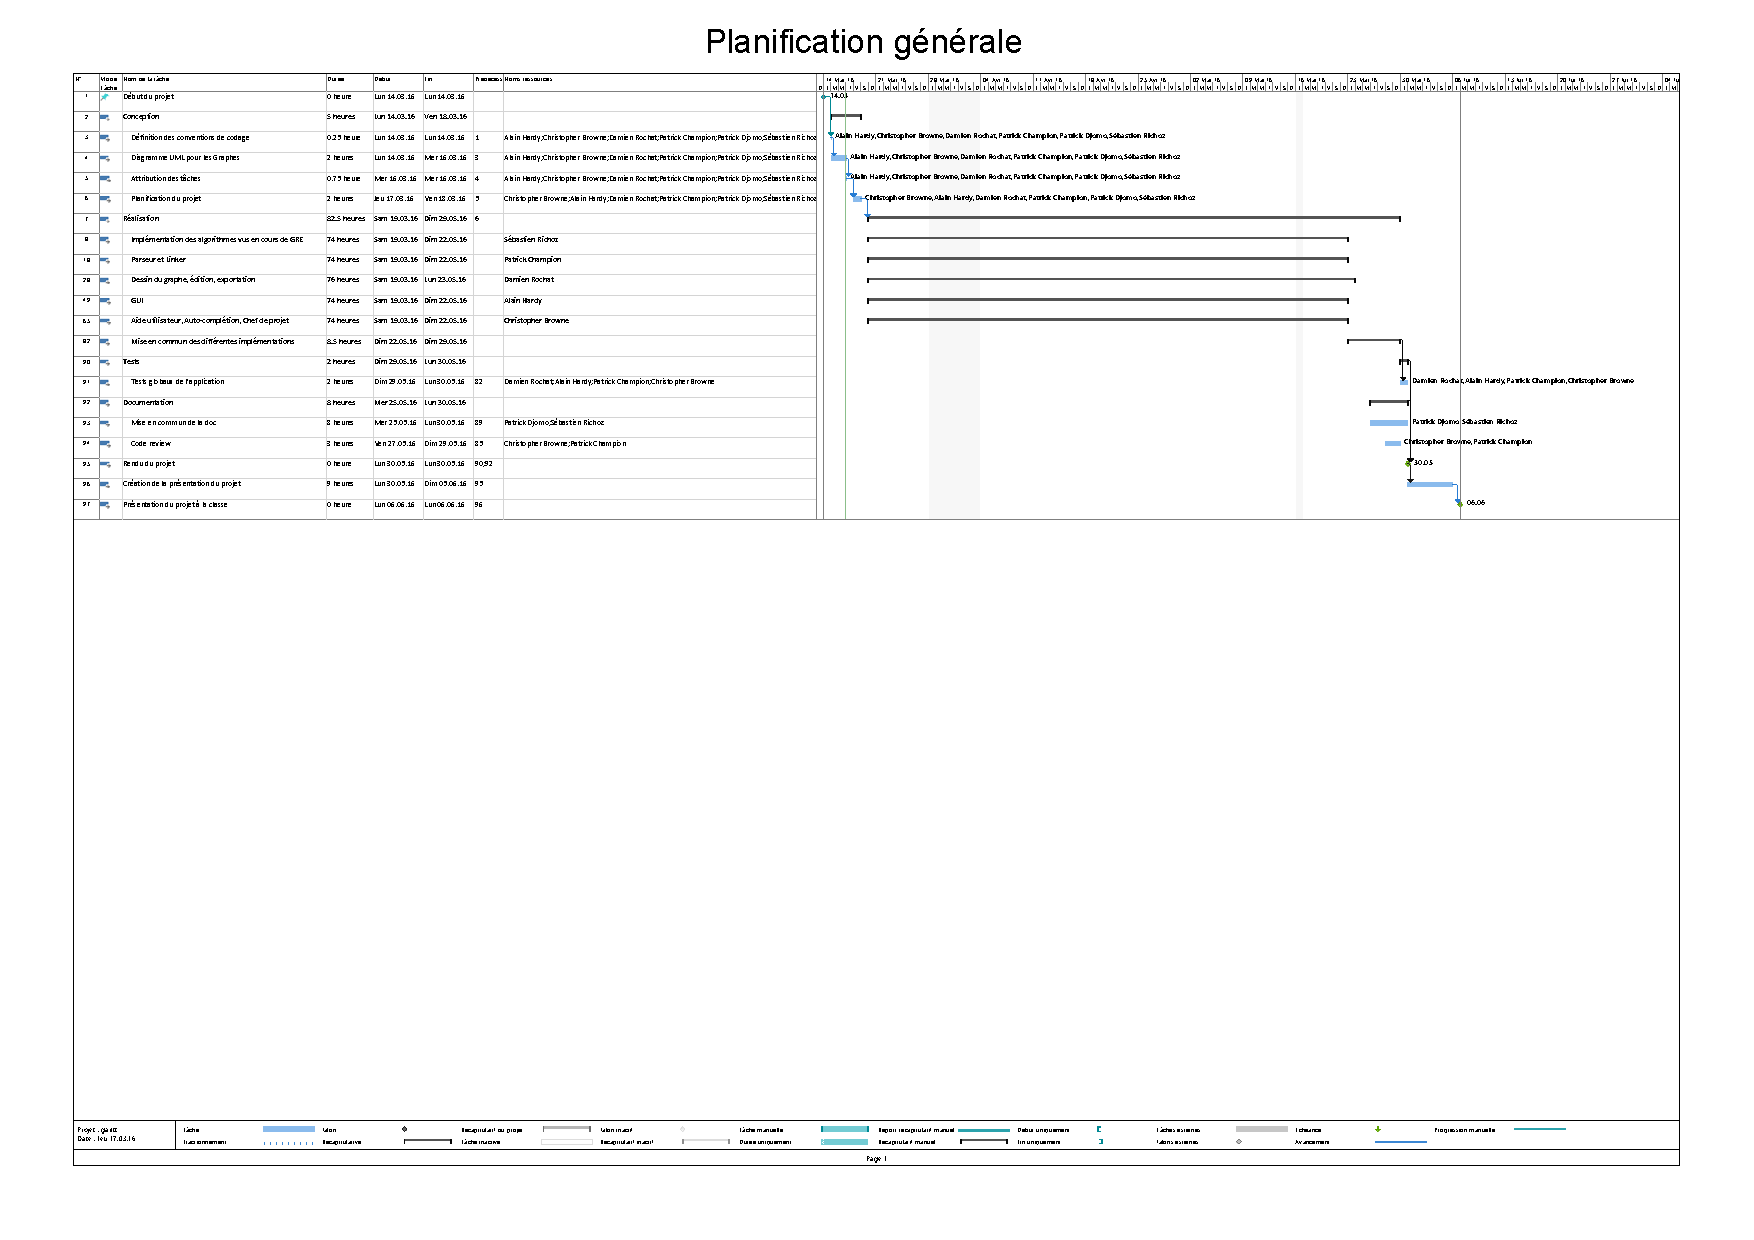
\includepdf[pages=1,angle=90,width=\textwidth]{Planification/gantt}	
			\includepdf[pages=2,angle=90,width=\textwidth]{Planification/gantt}	
			\includepdf[pages=3,angle=90,width=\textwidth]{Planification/gantt}	
			\includepdf[pages=4,angle=90,width=\textwidth]{Planification/gantt}	
			\includepdf[pages=5,angle=90,width=\textwidth]{Planification/gantt}	
			\includepdf[pages=6,width=\textwidth]{Planification/gantt}	

\end{document}
